\chapter{Dinámica Básica}

\section{Cinemática y Cinética}

\subsection{Cinemática de una partícula}

La mecánica es una rama de las ciencias físicas que se ocupa del estado de reposo o movimiento de cuerpos sometidos a la acción de fuerzas. 

La ingeniería mecánica se divide en dos áreas de estudio: la estática y la dinámica. La estática se ocupa del equilibrio de un cuerpo que está en reposo o que se mueve a velocidad constante. La dinámica se ocupa del movimiento acelerado de un cuerpo. 

La dinámica se divide en dos áreas de estudio: la dinámica y la dinámica.

\begin{enumerate}
    \item Cinemática, la cual trata sólo los aspectos geométricos del movimiento; 
    \item Cinética, que analiza las fuerzas que provocan el movimiento.
\end{enumerate}

Los principios de la cinemática relacionan el desplazamiento, la velocidad, la aceleración y el tiempo del movimiento de un cuerpo, sin referencia a la causa del movimiento.

La cinética se utiliza para predecir el movimiento ocasionado por fuerzas dadas o para determinar las fuerzas que se requieren para producir un movimiento específico

\subsubsection{Movimiento rectilíneo}

Una partícula que se mueve a lo largo de una línea recta, se dice que está en movimiento rectilíneo. Una partícula tiene masa, pero su tamaño y forma son despreciables. 

La cinemática de una partícula se caracteriza al especificar, en cualquier
instante, su posición, velocidad y aceleración. 

\begin{definition}[Posición]
    El origen $O$ en la trayectoria es un punto fijo, y a partir de él se utiliza la coordenada de posición $s$ para especificar la ubicación de la partícula en cualquier instante.
    La magnitud de $s$ es la distancia de $O$ a la partícula, por lo general medida en metros $(m)$ o pies. La posición es una cantidad vectorial.
\end{definition}

\begin{definition}[Desplazamiento]
    El desplazamiento de la partícula se define como el cambio en su posición.
    \begin{equation}
        \Delta S=s^{\prime}-s
    \end{equation}
    $\Delta s$ es positivo si $s^{\prime}>s$ y $\Delta s$ es negativo si $s^{\prime}<s$. El desplazamiento es una cantidad vectorial.
\end{definition}

La distancia recorrida es un escalar positivo que representa la longitud total de la trayectoria recorrida a lo largo de la cual viaja la partícula.

\begin{definition}[Velocidad]
    Si la partícula experimenta un desplazamiento $\Delta s$ durante el intervalo $\Delta t$, su velocidad promedio durante ese intervalo es:
    \begin{equation}
        v_{prom}=\frac{\Delta s}{\Delta t}
    \end{equation}
\end{definition}

La velocidad instantánea es un vector definido como:
\begin{equation}
    v=\lim_{\Delta t\to 0} \left(\frac{\Delta s}{\Delta t}\right)
\end{equation}
o bien, se puede expresar como:
\begin{notation}
    $v=\frac{d s}{d t}$
        El signo utilizado para definir el sentido de la velocidad es el mismo que el de $\Delta s$ o $ds$. La magnitud de la velocidad se conoce como \texttt{rapidez} y se expresa en unidades de $m/s$ ó $ft/s$
\end{notation}

\begin{definition}[Rapidez promedio]
    Es un escalar positivo y se define como la distancia total recorrida por la partícula, $S_T$, dividida entre el tiempo transcurrido $\Delta t$:
    \begin{equation}
        \left(v_{prom}\right)_{prom}=\frac{S_T}{\Delta t}
    \end{equation}
\end{definition}

\begin{definition}[Aceleración]
    Si se conoce la velocidad de la partícula en los puntos, su aceleración promedio durante el intervalo $\Delta t$ se define como:
    \begin{equation}
        A_{prom}=\frac{\Delta s}{\Delta t}
    \end{equation}
\end{definition}

donde $\Delta v=v^{\prime}-v$ es la diferencia de la velocidad durante el intervalo $\Delta t$. La aceleración instantánea en el instante $t$ se define como:
\begin{equation}
    a=\lim_{\Delta t\to 0} \left(\frac{\Delta v}{\Delta t}\right)
\end{equation}

\begin{notation}
    o bien de las siguientes formas:

    \begin{align*}
    &\left(\circlearrowright \right)&&a=\frac{dv}{dt}\\
    &\left(\circlearrowright \right)&&a=\frac{d^2 s}{d t^2}
    \end{align*}
\end{notation}


Tanto la aceleración promedio como la instantánea pueden ser positivas o negativas. Cuando la partícula se va moviendo cada vez más lentamente o su rapidez se reduce, se dice que se está desacelerando. Si la velocidad es constante, entonces la
aceleración es cero. Las unidades que se utilizan para expresar la magnitud de la aceleración son $m/s^2$ o $ft/s^2$.

Si eliminamos la diferencial de tiempo  $dt$ entre las ecuaciones $v=\frac{ds}{dt}$ y $a=\frac{dv}{dt}$, obtenemos:
\begin{equation}
    ads=vdv
\end{equation}

\begin{notation}
    Sobre la aceleración constante, $a=a_c$. Cuando la aceleración es constante, se pueden integrar las tres ecuaciones cinemáticas $a_c=\frac{dv}{dt}$, $v=\frac{ds}{dt}$ y $a_cds=vdv$ para obtener fórmulas que relacionan $a_c,v,s,t$
\end{notation}

\textbf{Velocidad en función del tiempo}. Integre $a_c=\frac{dv}{dt}$
considerando que inicialmente $v=v_0$ cuando $t=0$

\begin{align}
    &\int_{v_0}^{v}\, dv=\int_0^t a_c\, dt\\
    &v=v_0+a_ct\, \text{Aceleración constante}
\end{align}

\textbf{Posición en función del tiempo}. Integre $v=\frac{ds}{dt}=v_0+a_ct$
considerando que inicialmente $s=s_0$ cuando $t=0$

\begin{align}
    &\int_{s_0}^{s}\, ds=\int_0^t \left(v_0+a_ct\right)\, dt\\
    &s=s_0+v_0t+\frac{1}{2}a_c^2t^2\, \text{Aceleración constante}
\end{align}

\textbf{Velocidad en función de la posición} Integre $vdv=a_cds$, considerando que inicialmente $v=v_0$ cuando $s=s_0$

\begin{align}
    &\int_{v_0}^{v} v\, dv=\int_{s_0}^s a_c\, ds\\
    &v^2=v_0^2+2a_c\left(s-s_0\right)\, \text{Aceleración constante}
\end{align}

Éstas ecuaciones son útiles sólo cuando la aceleración es constante y cuando $t=0,s=s_0,v=s_0$. Un ejemplo típico de movimiento acelerado constante sucede cuando un cuerpo cae libremente hacia el suelo. 

La integración directa de las ecuaciones de movimiento es posible en los siguientes casos: 

Si $a=f(t)$, integramos $a=\frac{dv}{dt}$:
\begin{equation*}
\int_{v_0}^v\,dv=int_0^t f(t)\, dt
\end{equation*}

Integramos $v$ para obtener la posición $s$.

Si $a=f(v)$: Se integra $a=\frac{dv}{dt}$: 
\begin{equation*}
    \int_0^t \, dt=\int_{v_0}^v\frac{dv}{f(v)}
\end{equation*}

Integrar $ads=vdv$
\begin{equation*}
    \int_{s_0}^s\, ds=\int_{v_0}^v\frac{vdv}{f(v)}
\end{equation*}

Integrar $v$ para obtener la posición $s$, si $a=f(s)$, se integra $ads=vdv$: |
\begin{equation*}
    \int_{v_0}^v v\, dv=\int_{s_0}^s f(s)\, ds
\end{equation*}

\begin{example}
    La posición de una partícula que se mueve en línea recta está definida por $s=-3t^2+12t-6$m donde $t$ está en segundos y $m$ en metros. Para el intervalo de tiempo de $t=0$ a $t=3$, s:
    \begin{enumerate}
        \item Trace la gráfica de la posición, la velocidad y la aceleración como funciones del tiempo
        \item Calcule la distancia recorrida
        \item Determine el desplazamiento de la partícula 
    \end{enumerate}
\end{example}

\textit{ Sol. }

\begin{enumerate}
    \item \begin{align*}
        &s=-3t^2+12t-6\, m\\
        &v=\frac{ds}{dt}=-6t+12\, \frac{m}{s}
        &a=\frac{dv}{dt}=\frac{d^2s}{dt^2}=-6\, \frac{m}{s^2}
    \end{align*}
    
    Éstas funciones están graficadas en las figuras:
    
%    \begin{figure}[h!]
%      \centerline{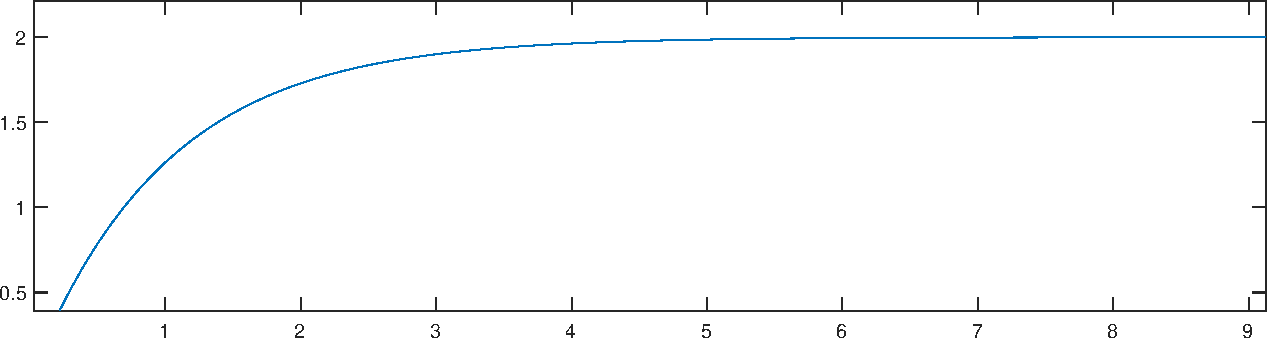
\includegraphics[width=0.5\textwidth]{db1.png}}
%      \caption{Posición}
%      \label{db1}
%    \end{figure}
%    
%    \begin{figure}[h!]
%        \centerline{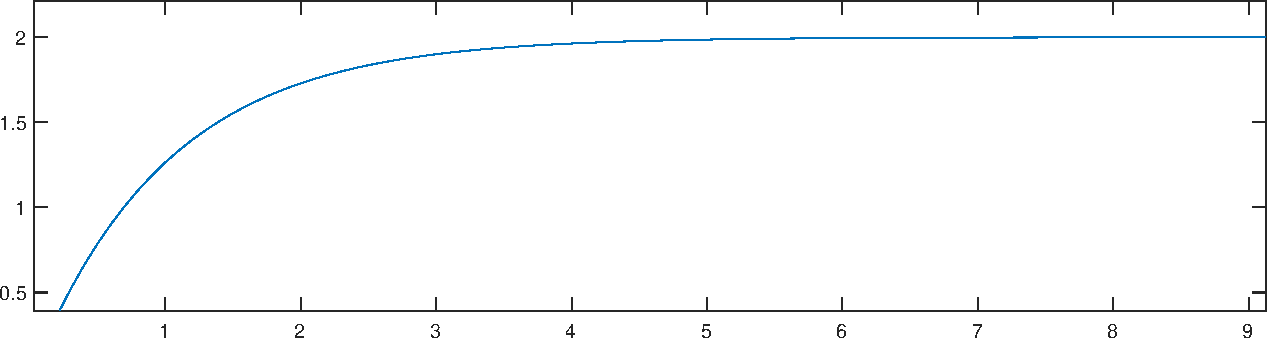
\includegraphics[width=0.5\textwidth]{db1.png}}
%        \caption{Posición}
%        \label{db2}
%      \end{figure}
%    
%    
%      \begin{figure}[h!]
%        \centerline{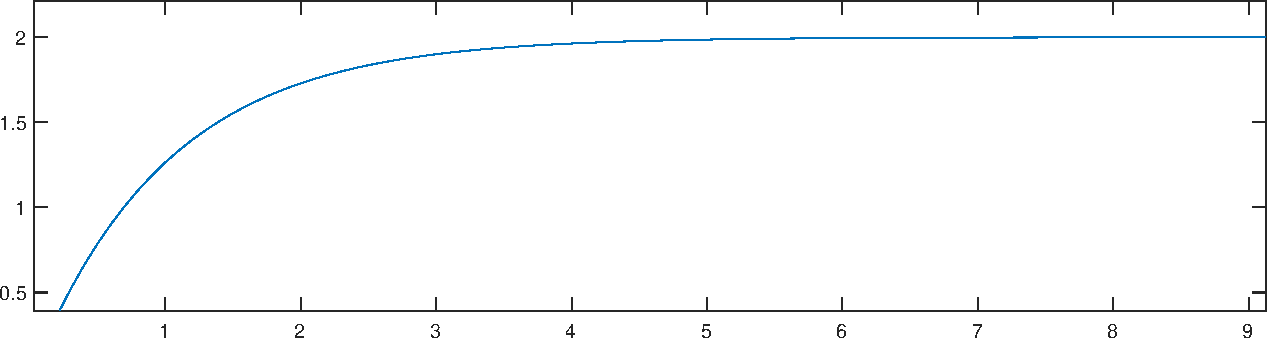
\includegraphics[width=0.5\textwidth]{db1.png}}
%        \caption{Posición}
%        \label{db3}
%      \end{figure}
%    \item Cuando $t=0$, la partícula parte de $s=-6$m y se mueve hacia la derecha. Cuando $t=2$s, la partícula se detiene en $s=6$m. Entonces se mueve hacia la izquierda, llegando a $s=3$m cuando $t=3$s.
%        \begin{equation*}
%            s_t=\left\lvert 6-(6)\right\rvert+\left\lvert 3-6\right\rvert =15
%        \end{equation*}

    \item El desplazamiento durante el intervalo de tiempo $t=0$ a $t=3$ es: 
    \begin{equation*}
        \Delta s=\left\lvert 6-(6)\right\rvert +(3-6)=12+3=9m
    \end{equation*}
    En formato vectorial: $\Delta r=9i$m
\end{enumerate}

\begin{example}
    Un automóvil se desplaza en línea recta, de modo que durante un corto tiempo su velocidad está definida por $v=\left(0.6t^2+t\right)$m/s, donde $t$ está en segundos. Determine su posición y aceleración en $t=3$s, si $t=0,s=0$.
\end{example}

\textit{ Sol. }

La posición se determina con $v=\frac{ds}{dt}$, con $s=0$ cuando $t=0$. 

\begin{align*}
    &v=\frac{ds}{dt}=\left(0.6t^2+t\right)\\ 
    &\int_0^s\, ds=\int_0^t\left(0.6t^2+t\right), dt\\
    &s=\left(0.2t^3+0.5t^2\right)m
\end{align*}
Cuando $t=3$s, $s=9.90$m 

La aceleración se determina con $a=\frac{dv}{dt}$

\begin{align*}
    &a=\frac{dv}{dt}=\frac{d\left(0.6t^2+2\right)}{dt}\\ 
    &a=\left(1.2t+1\right)\frac{m}{s^2}
\end{align*}

Cuando $t=3$s, $a=4.60\frac{m}{s^2}$


\begin{example}
    Una pelota se lanza con una velocidad de $10m/s$ dirigida verticalmente hacia arriba desde una ventana ubicada a 20m sobre el suelo. Si se sabe que la aceleración de la pelota es constante e igual a $9.81 m/s^2$ hacia abajo, determine: 
    \begin{enumerate}
        \item La velocidad $v$ y la elevación y de la pelota sobre el suelo en cualquier tiempo $t$ 
        \item La máxima elevación que alcanza la pelota y el valor correspondiente de $t$ 
        \item El tiempo en el que la pelota golpea el suelo y su velocidad correspondiente. Dibuje las curvas $v-t$ y $y-T$
    \end{enumerate}
\end{example}

\textit{ Sol. }

\begin{enumerate}
    \item \begin{align*}
        &a=\frac{dv}{dt}=\\
        &\int_{10}^v\, dv=-\int_0^t 9.81\, dt\\
        &v-10=-9.81t\\
        &v=10-9.81t\, m/s
    \end{align*}
    Al sustituir $v$ en $v=\frac{dy}{dt}$ en $t=0$, $y_0=20m$, se obtiene:
    \begin{align*}
        &v=\frac{dy}{dt}=10-9.81t
        &\int_{20}^{y}\,dy=int_0^t\left(10-9.81\right)\, dt
        &y-20=10t-4.905t^2\\ 
        &t=20+10t-1.905t^2m
    \end{align*}
    \item \textbf{Máxima elevación:} Cuando la pelota alcanza su máxima elevación, $v=0$. Al sustituir en la ecuación de velocidad, 
    \begin{align*}
        &10-9.81t=0\\
        &t=1.019s
    \end{align*}
    Al sustituir $t=1.019s$ en la ecuación de la posición, obtenemos:
    \begin{align*}
        &y=20+10(1.019)-4.905(1.019)^2m\\
        &y=25.1m
    \end{align*}
    \item \textbf{La pelota golpea el suelo:} Cuando la pelota golpea el suelo, $y=0$ Al sustituir en la ecuación de posición: 
    \begin{align*}
        &0=20+10t-4.905t^2\\
        &\text{Raíces: }t=-1.243s,\, t=3.28s 
    \end{align*}
    Sólo la raíz $t=3.28$s corresponde a un tiempo positivo, sustituye este valor $t$ en la ecuación de velocidad: 
    \begin{align*}
        &v=10-9.81(3.28)=-22.2m/s\\
        &v=22.2m/s\downarrow
    \end{align*} 
\end{enumerate}

Utilizando las fórmulas obtenidas con aceleración constante. 

\begin{enumerate}
    \item \textbf{Velocidad y posición}
    Velocidad:
\begin{equation*}
    v=v_0+a_c
\end{equation*}
Sustituyendo los datos, $a_c=-9.81m/s^2$, entonces
\begin{align*}
    &v_0=10m/s\mid t=0\\
    &v=10 m/s-9.81tm/s^2
\end{align*}

Elevación: 
\begin{align*}
    &t=t_0+v_0t0\frac{1}{2}a_ct^2m\\
    &y=20+10t+\frac{1}{2}-9.81t^2m\\
    &y=20+10t-4.905t^2m
\end{align*}
    \item \textbf{Máxima elevación}
    
    Punto $A=$ posición inicial. Punto $B=$ máxima elevación. Punto $C=$ punto de contacto con el suelo.

Usando la fórmula, con $v_B=0m/s$: 
\begin{align*}
    &v^2+v_0^2+2a_c\left(s-s_0\right)\\
    &v_B^2=v_A^2+2a_c\left(s_B-s_A\right)\\
    &0=\left(10\right)^2+2\left(-9.81m/s^2\right)\left(s_B-20m\right)\\
    &s_B=25.1m
\end{align*}

El tiempo $t$, $v=v_0+a_ct$. $0=10+9.81tm/s,t=1.019s$

\item \textbf{La pelota golpea el suelo}
\begin{equation*}
    v_c^2=v_B^2+2a_c\left(s_C-s_B\right)
\end{equation*}
Sustituyendo los datos: 
\begin{align*}
    &v_C^2=0+2(-9.81)(0-25.1)\\
    &v=\sqrt{492.462}\\
    &v=-22.19m/s\, v=22.19m/s\\
    &\therefore v=22.2m/s\downarrow
\end{align*}

Tiempo cuando la pelota golpea el suelo, usando la ecuación de velocidad y $v=-22.2m/s\implies -22.2=10-9.81tm/s\implies t=3.28s$
\end{enumerate}

\begin{example}
    Muchos amortiguadores para bicicleta de montaña utilizan un pistón que se mueve dentro de un cilindro lleno de aceite para proporcionar amortiguación.
    Cuando la rueda delantera pasa por un montículo, el cilindro recibe una velocidad inicial de $v_0$. El pistón, que está unido a la horquilla, se mueve con respecto al cilindro y el aceite es forzado a través de los orificios del pistón. Esto hace que el pistón se desacelera a una razón proporcional a la velocidad, $a=-kv$. En el momento $t=0$, la posición del pistón es $x=0$
    \begin{enumerate}
        \item Velocidad en términos del tiempo
        \item La posición $x$ en términos de $t$
        \item La velocidad en términos de $x$
    \end{enumerate}
\end{example}

\textit{ Sol. }

\begin{enumerate}
    \item $v$ en términos de $t$. Al sustituir $a=-kv$ en la definición de aceleración, $a=\frac{dv}{dt}$

    \begin{align*}
        &a=\frac{dv}{dt}=-kv\\
        &\frac{dv}{v}=-k\, dt\\
        &\int_{v0}^{v}=-k\int_0^t\, dt\\
        &\ln{\left(\frac{v}{v_0}\right)}=-kt\\
        &\frac{v}{v0}=e^{-kt}\\
        &\frac{v}{v0}=e^{-kt}\\
        &v=v_0e^{-kt}\,m/s
    \end{align*}

    \item $x$ en términos de $t$. Al sustituir la expresión de la velocidad que se acaba de obtener para $v$ en $v=\frac{dx}{dt}$

    \begin{align*}
        &v=\frac{dx}{dt}=v_0e^{-kt}\\
        &\int_0^x\,dx=v_0\int_0^te^{-kt}\, dt\\
        &x=-\frac{v_0}{k} e^{-kt}\mid_0^t=-\frac{v_0}{k}\left(e^{-kt}-1 \right)\\
        &x=\frac{v_0}{k}\left(1-e^{-kt}\right)
    \end{align*}
    
    \begin{figure}[h!]
        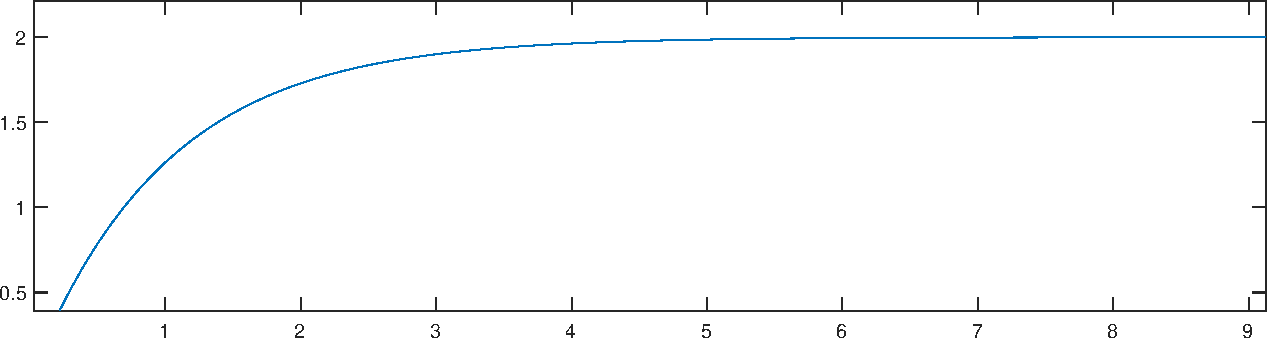
\includegraphics[scale=0.5]{db1.pdf}
        \caption{Comportamiento de la x en términos de t}
        \label{db1}
    \end{figure}
    
    \item $v$ en términos de $x$. Al sustituir $a=-kv$ en $a\,dx=v\,dv$

    \begin{align*}
        &a\,dx=v\,dv\\ 
        &a=v\frac{dv}{dx}\\
        &-kv=v\frac{dv}{dx}\\ 
        &-k\,dx=dv\\ 
        &-k\int_0^x\,dx=\int_{v_0}^v\,dv\\ 
        &-kx=v-v_0\\ 
        &v=v_0-kx
    \end{align*}
    \begin{figure}[h!]
        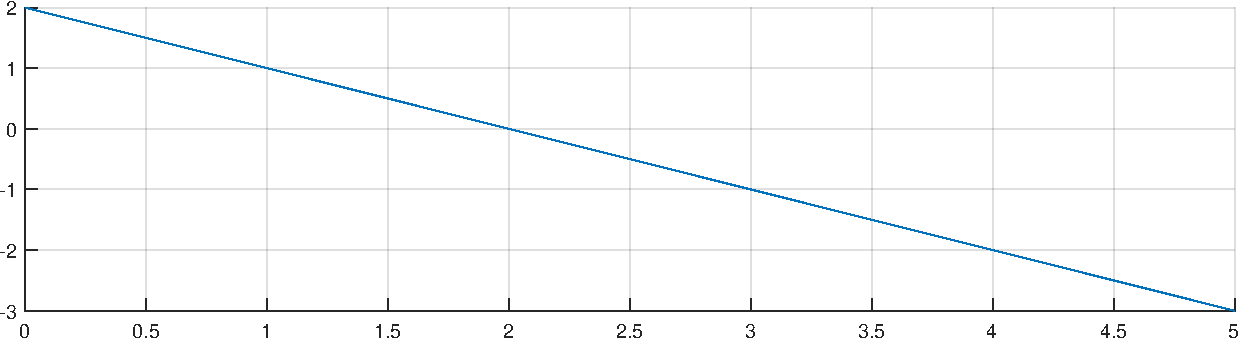
\includegraphics[scale=0.5]{db2.pdf}
        \caption{Comportamiento de la x en términos de v}
        \label{db2}
    \end{figure}
\end{enumerate}

\begin{problem}[La aceleración de un cohete]
    que viaja hacia arriba está dada por $a=(6+0.02s)m/s^2$ donde $s$ se da en metros. 
    Determine el tiempo necesario para que el cohete llegue a una altitud de $s=100m$. Inicialmente $v=0$ y $s=0$ cuando $t=0$
\end{problem}

\textit{ Sol. }

En este caso $a=f(s)$, la velocidad se determina con $ads=v\,dv$

\begin{align*}
    &v\,dv=a\,ds\\ 
    &\int_0^v v\,dv=\int_0^s(6+0.02s)\,ds\\
    &\frac{1}{2}v^2=6s+0.01s^2\\
    &v=\sqrt{2(6s+0.01s^2)}\\
    &v=\sqrt{12s+0.02s^2}
\end{align*}
Ahora integramos $v=\frac{ds}{dt}$ para obtener la posición.
\begin{align*}
    &dt=\frac{ds}{v}\\
    &\int_0^t\,dt=\int_0^{100}\frac{ds}{\sqrt{12s+0.02s^2}}\\
\end{align*}
Aplicando la fórmula de las integrales.

\begin{align*}
    \frac{1}{\sqrt{0.02}}\ln{\left(\sqrt{12s+0.02s^2}+s\sqrt{0.02}+\frac{12}{2\sqrt{0.02}}\right)}\mid_0^{100}\\ 
    t=5.62s
\end{align*}

\subsubsection{Movimiento curvilíneo general}

\begin{definition}[Movimiento curvilíneo]
    Ocurre cuando una partícula se desplaza a lo largo de una trayectoria curva
\end{definition}

\begin{definition}[Posición]
    El vector de posición $r=r(t)$ designará la posición de la partícula, medida con respecto a un punto fijo 0
\end{definition}

\begin{definition}[Desplazamiento]
    El desplazamiento $\Delta r$ representa el cambio de posición de la partícula y se determina mediante una recta vectorial $\Delta r=r^{\prime}-r$
\end{definition}

\begin{definition}[Velocidad]
    Durante el tiempo $\Delta t$ la velocidad promedio de la partícula es: 
    \begin{equation}
        v_{prom}=\frac{\Delta r}{\Delta t}
    \end{equation}
\end{definition}

La velocidad instantánea se determina con ésta ecuación cuando $\Delta t\to 0, v=\lim_{\Delta to 0}\left(\frac{\Delta}{\Delta t}\right)$ ó 
\begin{equation}
    v=\frac{dr}{dt}
\end{equation}

Como $dr$ será tangente a la curva, la dirección de $v$ también es tangente a la curva.

La magnitud de $v$, la rapidez, se obtiene al considerar que la longitud del segmento de línea recta $\Delta r=r^{\prime}-r$

\begin{figure}[h!]
    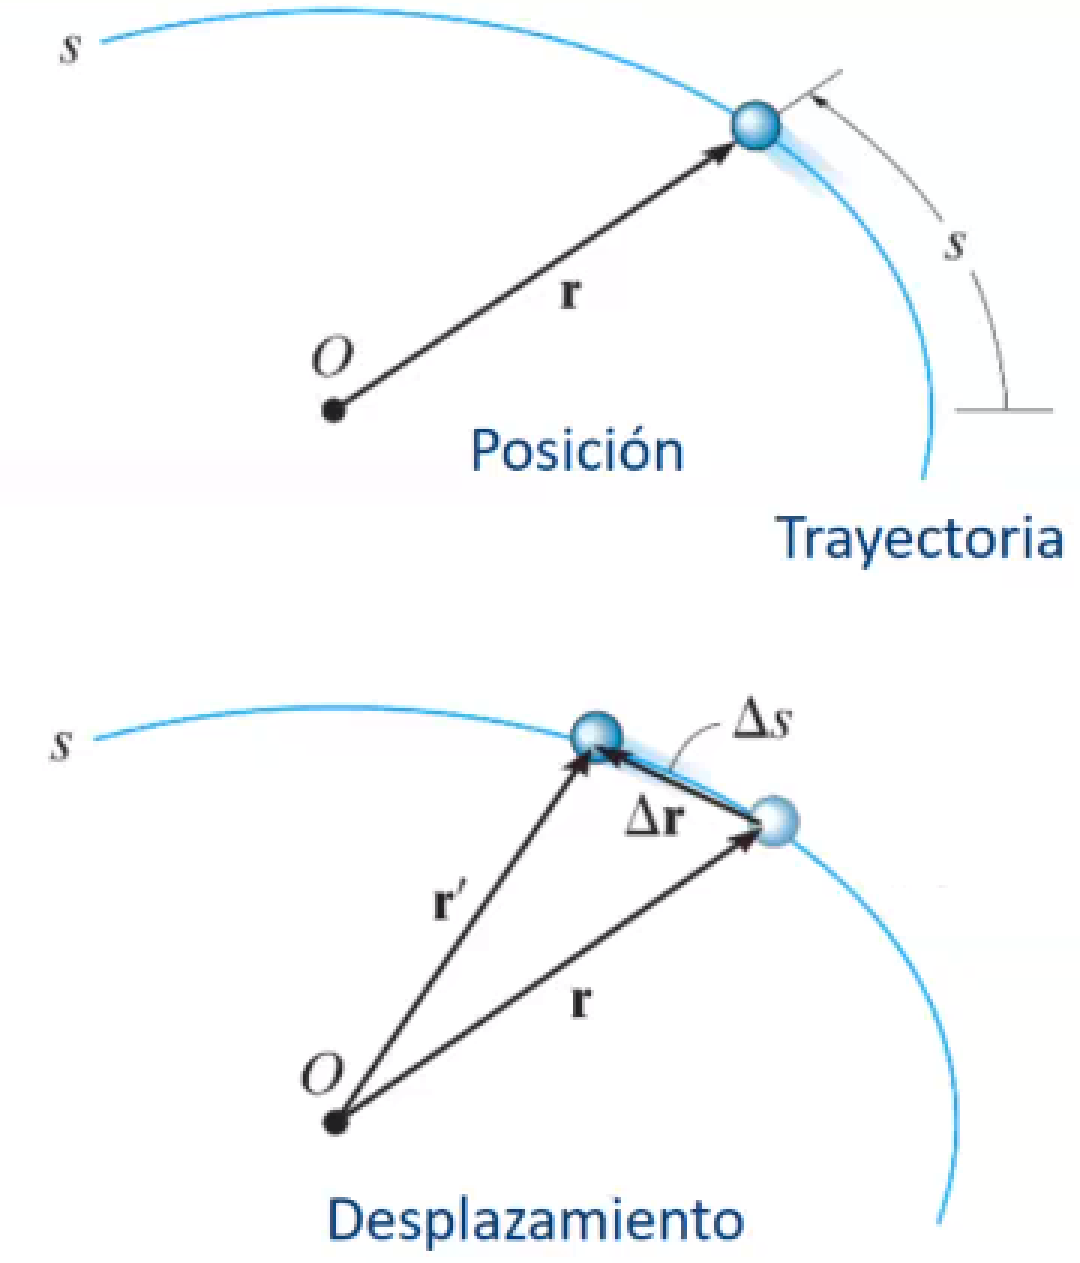
\includegraphics{db3.png}
    \caption{Movimiento curvilíneo general}
    \label{db3}
\end{figure}
\begin{equation}
    v=\lim_{\Delta t\to 0}\left(\frac{\Delta r}{\Delta t}\right)=\lim_{\Delta t\to 0}\left(\frac{\Delta s}{\Delta t}\right)
\end{equation}

\begin{definition}[Aceleración]
    Si la velocidad de la partícula es $v$ en el instante $t$ y la velocidad es $v^{\prime}=v+\Delta v$ en el instante $t+\Delta t$, entonces la aceleración promedio de la partícula durante el intervalo es: 
    \begin{equation}
        a_{prom}=\frac{\Delta v}{\Delta t}
    \end{equation}
    Donde $\Delta v=v^{\prime}-v$ para obtener la aceleración instantánea se hace $\Delta t\to 0, a=\lim_{\Delta t\to 0}\left(\frac{\Delta v}{\Delta t}\right)$.
    o bien:
    \begin{equation}
        a=\frac{dv}{dt}=\frac{d^2r}{dt^2}
    \end{equation}
\end{definition}

La primera derivada con respecto al tiempo de r proporciona la velocidad de la partícula

\begin{align*}
    &v=\frac{dr}{dt}=\frac{d}{dt}(xi)+\frac{d}{dt}(yj)+\frac{d}{dt}(zk)\\ 
    &\frac{d}{dt}(x\hat{i})=\frac{dx}{dt}\hat{i}+\frac{d\hat{i}}{dt}y\quad \frac{d\hat{i}}{dt}=0\\
    &v=\frac{dr}{dt}=v_x\hat{i}+v_y\hat{j}+v_z\hat{k}
\end{align*}
Donde $v_x=x,v_y=y,v_z=z$ La magnitud de la velocidad se determina como: 
\begin{equation}
    v=\sqrt{v_x^2+v_y^2+v_z^2}
\end{equation}
Y el vector unitario $u_v=\frac{v}{v}$ especifica su dirección. Esta siempre es tangente a la trayectoria\footnote{Puede verse más profundidad en el capítulo de Cálculo Multivariado}

La aceleración se obtiene de la primera derivada con respecto al tiempo de $v$ o la segunda derivada con respecto al tiempo de $r$. 
\begin{equation}
    a=\frac{dv}{dt}=a_x\hat{i}+a_y\hat{j}+a_z\hat{k}\\
\end{equation}


\begin{example}
    En cualquier instante la posición horizontal del globo meteorológico es definido por $x=(2t)$ donde $t$ está en segundos. Si la educación de la trayectoria es $y=\frac{x^2}{5}$ determine la magnitud y la dirección de la velocidad  la aceleración cuando $t=2$
\end{example}
\begin{figure}[h!]
  \centerline{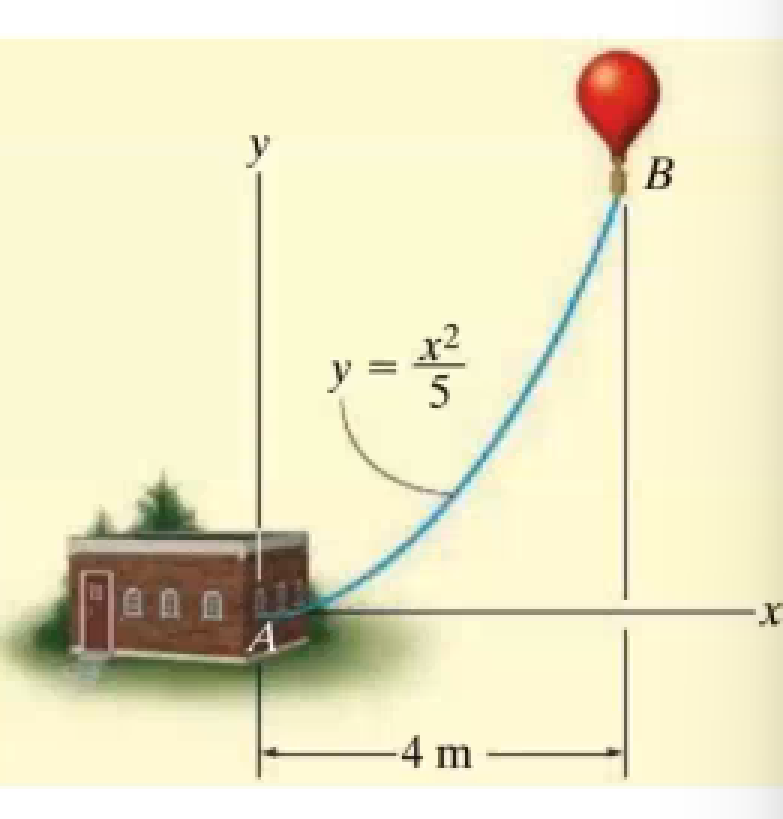
\includegraphics[width=0.5\textwidth]{db4.png}}
  \caption{Esquema del ejemplo}
  \label{db4}
\end{figure}
\textit{ Sol. }

Velocidad: Componente de la velocidad en la dirección $x$
\begin{equation*}
    v_x=\dot{x}=\frac{d}{dt}(2t)=2m/s\\ 
\end{equation*}

Componente de la velocidad en la dirección $y$
\begin{equation*}
    v_y=\dot{y}=\frac{d}{dt}\left(\frac{x^2}{5}\right)=2x\cdot \frac{\dot{x}}{5}
\end{equation*}

Cuando $t=2s$, $x=2(2)=4$. Sustituyendo los valores de $x$ y $\dot{x}$ cuando $t=2s$ en $v_y$.

\begin{align*}
    &v_y=\frac{2x\cdot \dot{x}}{5}=\frac{(2)(8)}{5}=3.20m/s\\
    &\text{La magnitud de la velocidad cuando }t=2s\\
    &v=\sqrt{(2m/s)^2+(3.20m/s)^2}=3.77m/s\\
    &\text{La dirección de v es tangente a la trayectoria}.\\
    &\theta_v=\arctan{\left(\frac{v_y}{v_x}\right)}=\arctan{\left(\frac{3.20}{2}\right)}=58.0^{\circ}
\end{align*}
aceleración
\begin{align*}
    &a_x=\dot{v}_x=\frac{d}{dt}(2)=0m/s^2\\
    &a_y=\dot{v}_y=\frac{d}{dt}\left(\frac{2x\cdot \dot{x}}{5}\right)=\frac{2(\dot{x})(x)}{5}=\frac{2(\dot{x})(\dot{x})}{5}+\frac{2(\dot{x})(\dot{x})}{5}\\
    &a_y=\frac{2(2)(2)}{5}+\frac{2(4)(0)}{5}=1.60m/s^2\\
    &a=\sqrt{0+(1.60)^2}=1.60m/s^2\\
    &\theta_a=\arctan{\left(\frac{a_y}{a_x}\right)}=\arctan{\frac{1.60}{0}}\\
    &\theta_a=90^{\circ}
\end{align*}

\begin{figure}[h!]
  \centerline{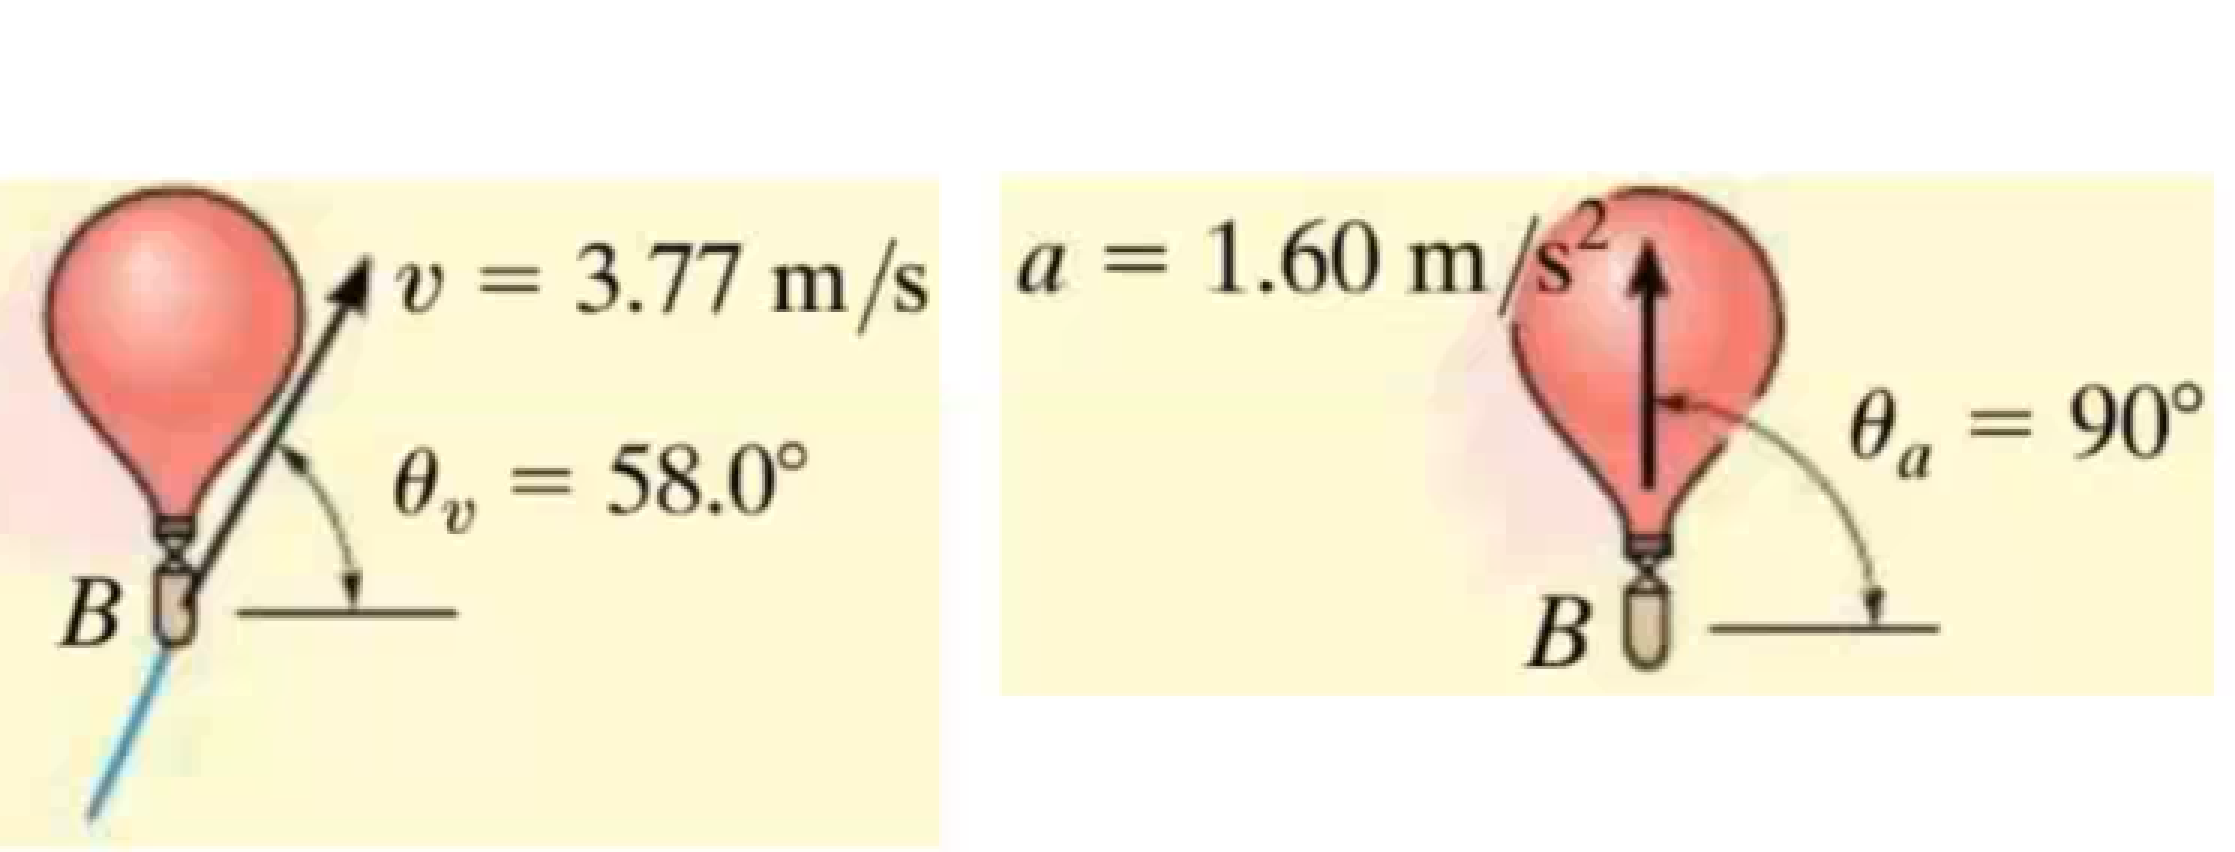
\includegraphics[width=0.5\textwidth]{db5.png}}
  \caption{Esquema del resultado}
  \label{db5}
\end{figure}

\subsubsection{Movimiento de un proyectil}

Considere un proyectil lanzado desde el punto $(x_0,y_0)$, con la velocidad inicial de $v_0$, cuyas componentes son $(v_0)_x$ y $(v_0)_y$.
Cuando se desprecia la resistencia del aire, la única fuerza que actúa en el proyectil es su peso, el cual hace que el proyectil tenga una aceleración dirigida hacia abajo constante de aproximadamente
$a_c=g=9.82m/s^2$ o bien $g=32.2ft/s^2$.

\begin{figure}[h!]
  \centerline{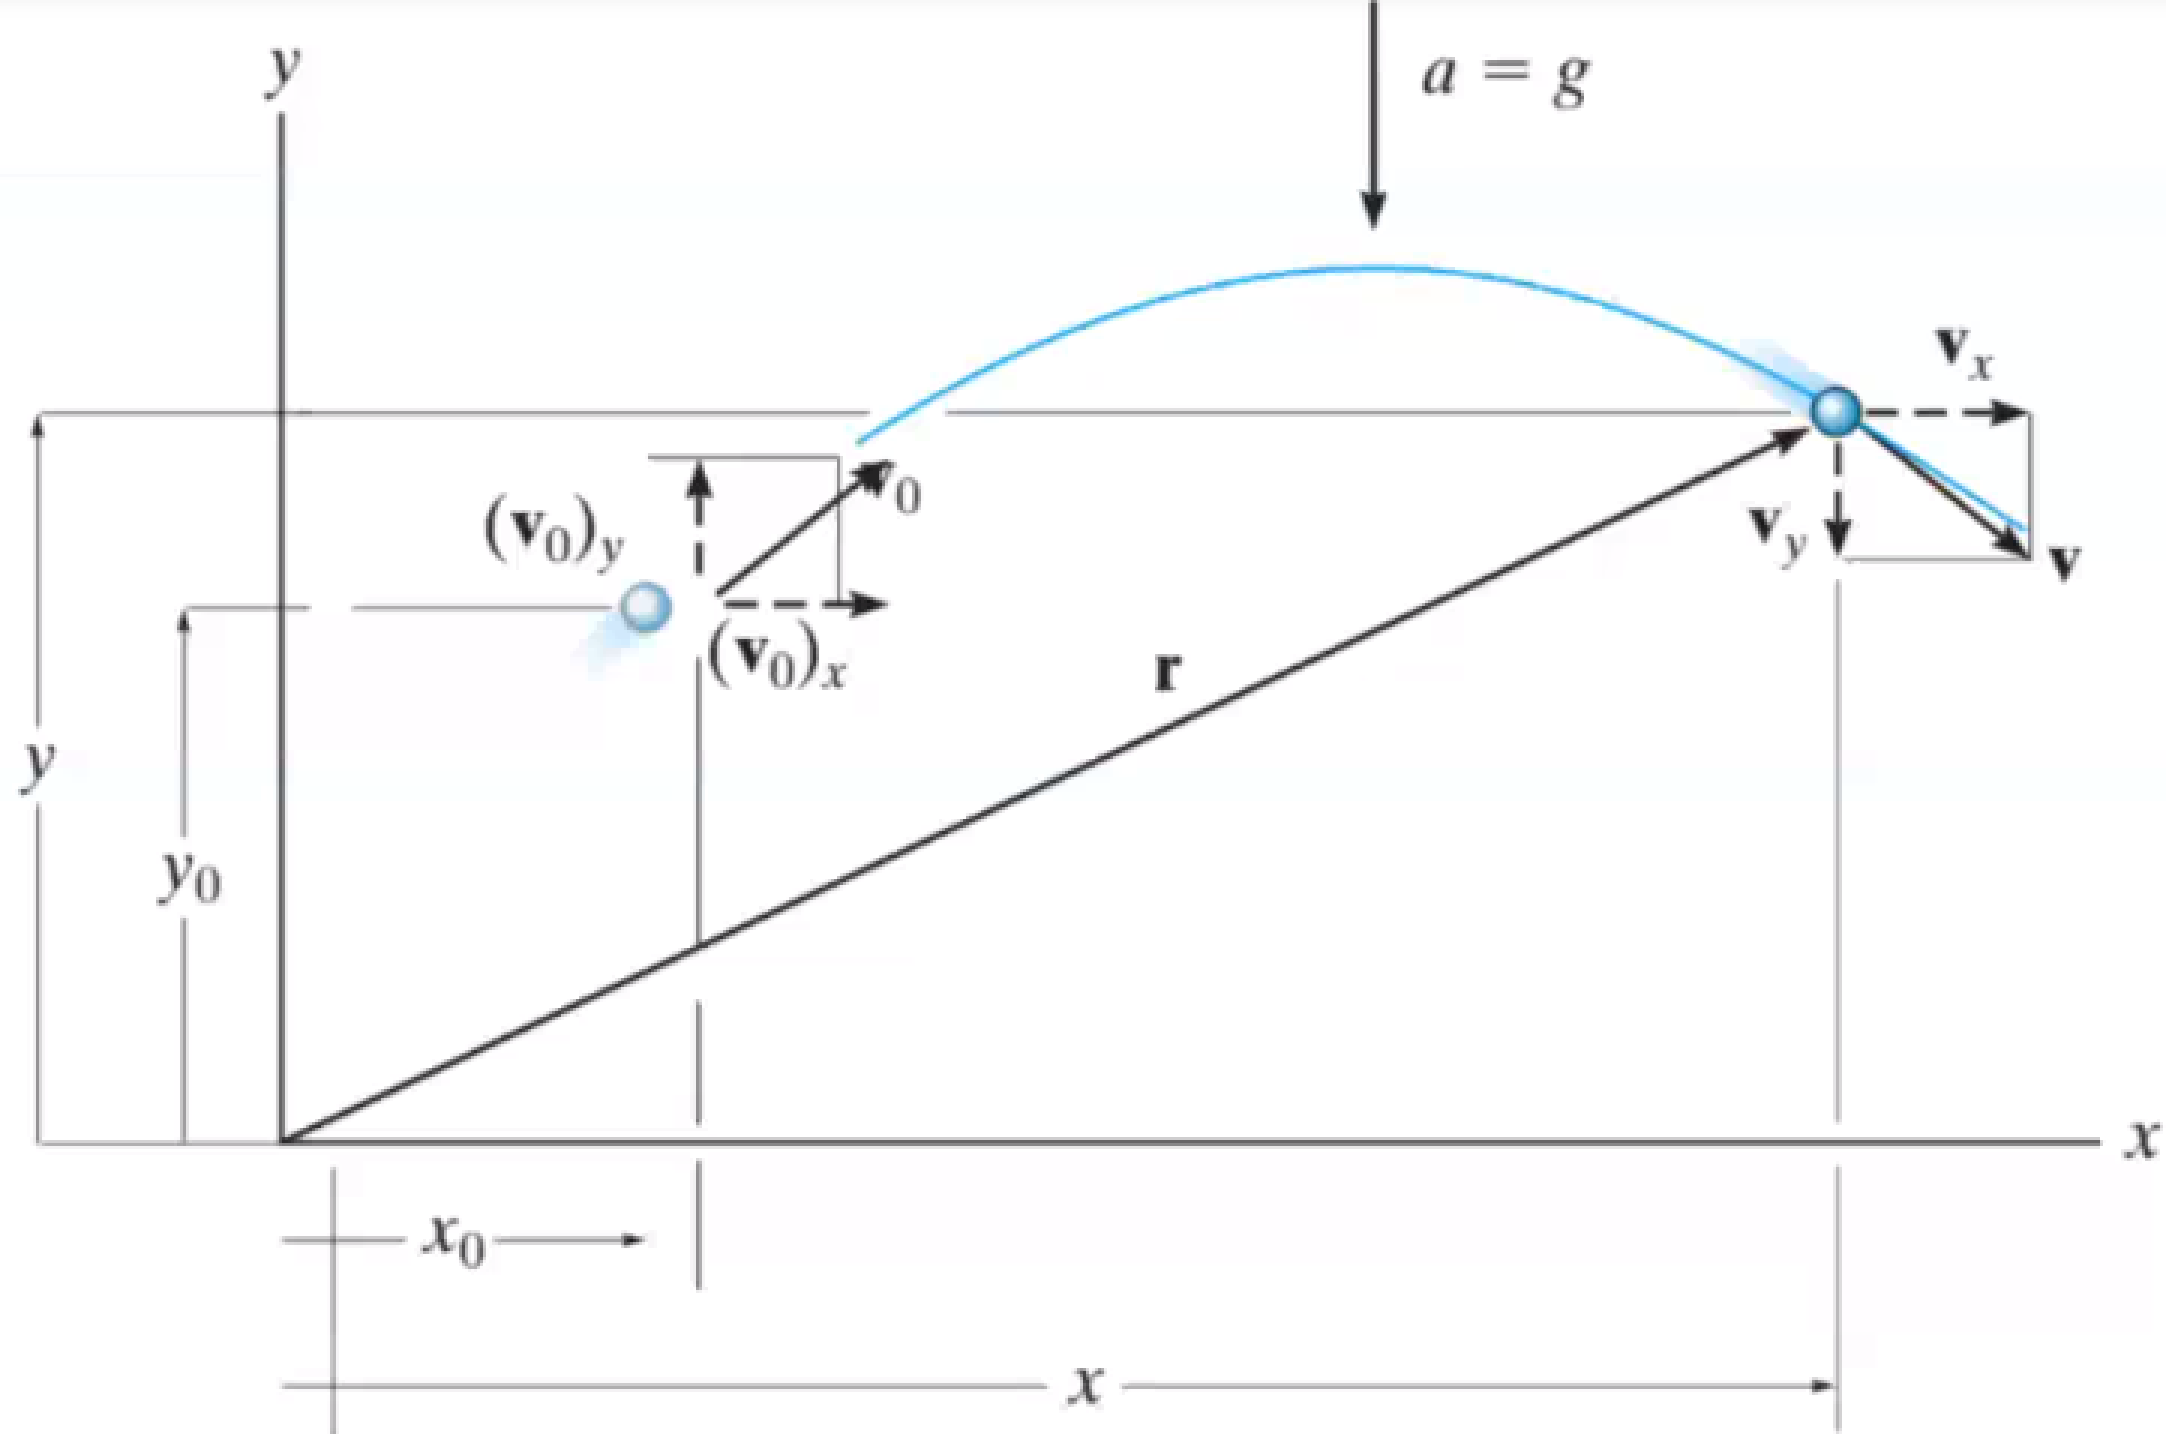
\includegraphics[width=0.5\textwidth]{db6.png}}
  \caption{Movimiento de un proyectil, en la ingeniería en irrigación, puede describir el movimiento de agua de un aspersor}
  \label{db6}
\end{figure}

El movimiento horizontal, como $a_c=0$, la aplicación de las ecuaciones de aceleración constante resulta en: 

\begin{align*}
&\left(\overset{+}{\longrightarrow }\right)v=v_0+a_ct&&v_x=(v_0)_x\\
&\left(\overset{+}{\longrightarrow }\right)x=x_0+v_0t+\frac{1}{2}a_ct^2&&x_x=x_0+(v_0)_xt\\
&\left(\overset{+}{\longrightarrow }\right)v^2=v_0^2+2a_c\left(x-x_0\right)&&v_x=(v_0)_x
\end{align*}
La componente horizontal de la velocidad siempre permanece constante durante el movimiento

Movimiento vertical. Como el eje $y$ positivo, está dirigido hacia arriba, entonces $a_y=-g$. Al aplicar las ecuaciones de aceleración constante, obtenemos:

\begin{align*}
    &(+\uparrow )v=v_0+a_ct&&v_y=(v_0)_y-gt\\
    &(+\uparrow )y=y_0+v_0t+\frac{1}{2}a_ct^2&&y=y_0+(v_0)_yt-\frac{1}{2}gt^2\\
    &(+\uparrow )v^2=v_0^2+1a_x\left(y-y_0\right)&&v^2_y=(v_0)^2_y-g\left(y-y_0\right)
\end{align*}

Los problemas que implican el movimiento vertical de un proyectil pueden tener como mucho tres incógnitas, una ecuación en la dirección horizontal y dos en la dirección vertical 
Una vez obtenidas $v_x$ y $v_y$, la velocidad resultante $v$, la cual siempre es tangente a la trayectoria, se determina mediante la suma vectorial.

\begin{example}
    La máquina desmenuzadora está diseñada para expulsar virutas de madera a $v_0=7.5m/s$. Si el tubo está orientado a $30^{\circ}$ con respecto a la horizontal, determine a qué altura, $h$, las virutas chocan contra la pila, si en este instante caen en la pila a $6m$ del tubo
\end{example}

\begin{figure}[h!]
  \centerline{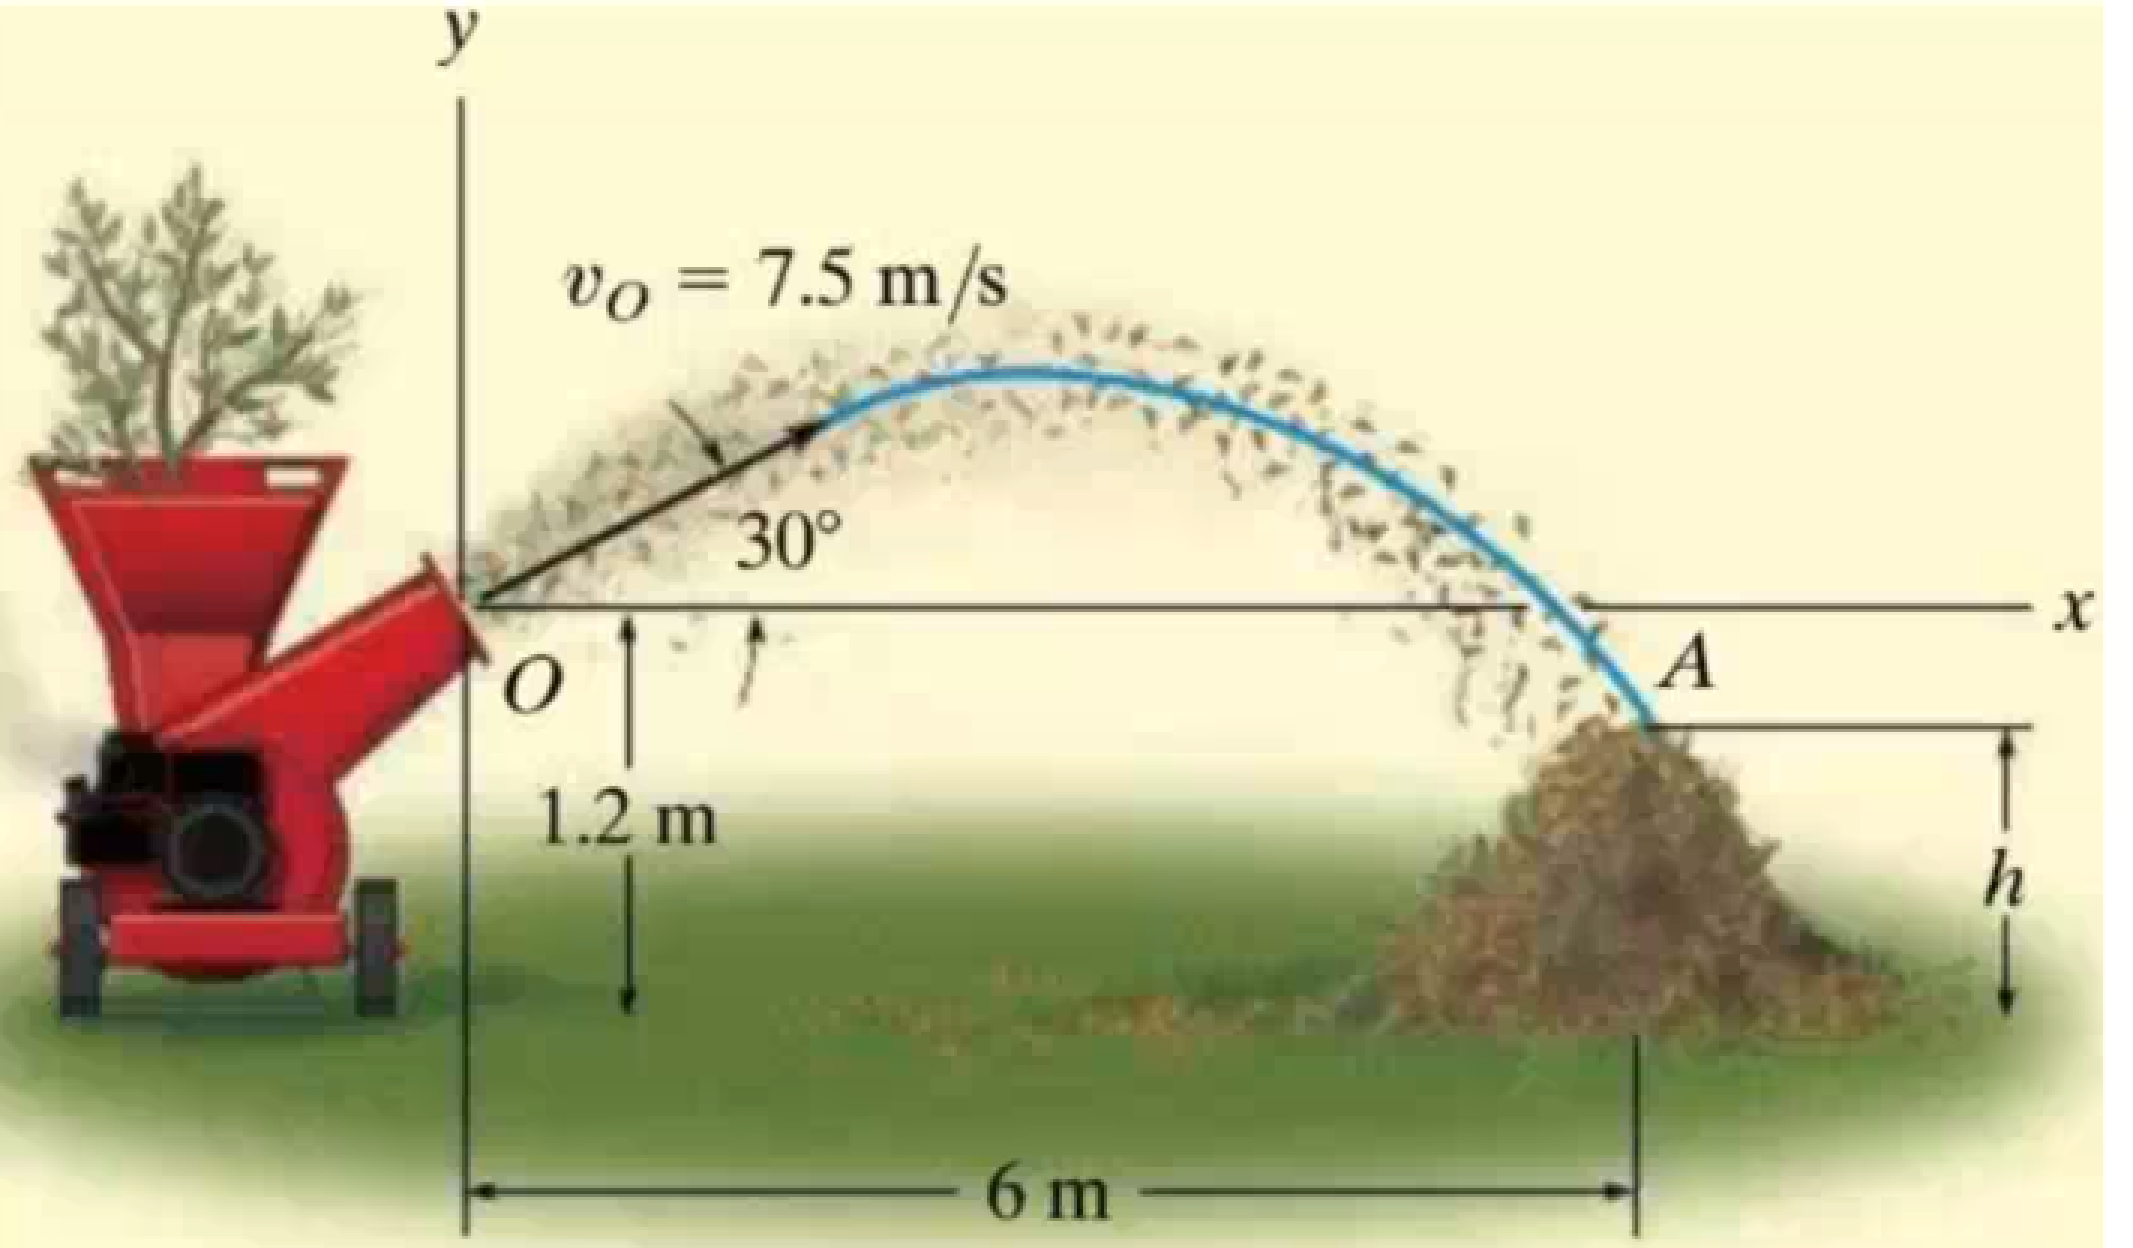
\includegraphics[width=0.5\textwidth]{db7.png}}
  \caption{Dibujo del problema}
  \label{db7}
\end{figure}

\textit{ Sol. }

Los sistemas de coordenadas, componentes de la velocidad inicial son: 

\begin{align*}
    &(v_0)_x=(7.5\cos{(30^{\circ})})=6.50m/s\\
    &(v_0)_y=(7.5\sin{(30^{\circ})})=3.75m/s\\
    &v_x=(v_0)_x=6.5m/s\, a_y=g=-9.81m/s^2
\end{align*}
Para el movimiento horizontal
\begin{align*}
    &6m=0+(6.50)t_{0A}&&(v_A)_y=3.75m/s+(-9.81m/s^2)(0.923s)\\
    &t_{0A}=0.923s&&(v_A)_y=-5.30m/s
\end{align*}
Movimiento vertical: 
\begin{align*}
    &(h-1.2m)=0+(3.75m/s)(0.923s)+\frac{1}{2}(-9.81m/s^2)(0.923s)^2\\
    &h=0.482m
\end{align*}

\begin{example}
    Un proyectil se lanza desde el borde de un acantilado de 159m con una velocidad inicial de 180 m/s a un ángulo de $30^{\circ}$ con la horizontal. SI se ignora la resistencia del aire, encuentre: 
    \begin{enumerate}
        \item La distancia horizontal desde el cañón hasta el punto en el que el proyectil golpea el suelo
        \item La elevación máxima sobre el suelo que alcanza el proyectil
    \end{enumerate}
\end{example}
\begin{figure}[h!]
  \centerline{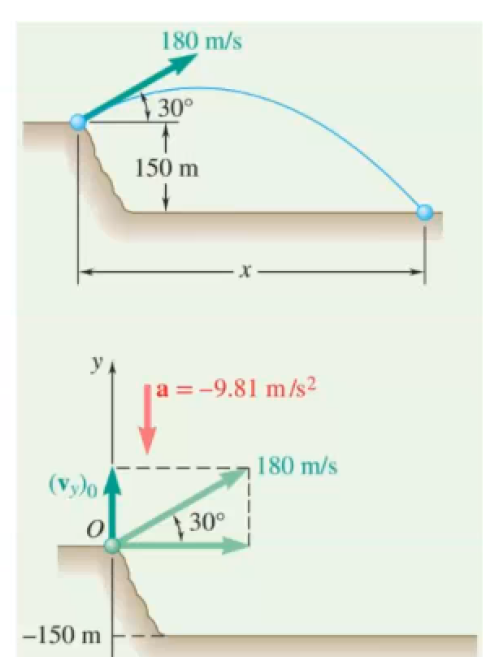
\includegraphics[width=0.5\textwidth]{db8.png}}
  \caption{Esquema del problema}
  \label{db8}
\end{figure}
\textit{ Sol. }
Componentes de la velocidad inicial
\begin{align*}
    &(v_0)_x=180\cos{(30^{\circ})}=155.88m/s\\
    &(v_0)_y=180\sin{(30^{\circ})}=90m/s\\
    &a_c=g=-9.81m/s^2
\end{align*}
Movimiento vertical
\begin{align*}
    &v_y=(v_0)_y+gt\\
    &v_y=80-9.81t
\end{align*}

\begin{align*}
    &y=0+90t+\frac{1}{2}(-9.81)t^2\\
    &y=90t-4.905t^2\\
    &v_y^2=(v_0)^2_y-2g(y-y_0)\\
    &v_y^2=(90)^2+2(-9.81)(y-0)\\
    &v_y^2=8100-19.62y
\end{align*}

Movimiento horizontal

\begin{align*}
    &v_x=(v_0)_x=155.88m/s\\
    &x=0+155.88t\\
    &x=155.88t
\end{align*}

Distancia horizontal

\begin{align*}
    &y=-150m\\
    &-150=90t-1.908t^2\\
    &0=150+90t-4.905t^2\\
    &t=19.9s
\end{align*}
Sustituyendo en la ecuación de movimiento vertical
\begin{equation*}
    x=155.88(19.9)=3102m
\end{equation*}
La elevación máxima es cuando $v_y=0$
\begin{align*}
    0^2=8100-19.62y\implies y==413m
\end{align*}
La máxima elevación es 413m+150m=563m

\begin{example}
    El análisis de la trayectoria de un proyectil cuando se lanza sobre un plano inclinado, es muy similar a lo descrito para un plano no inclinado. En tales casos, el sistema coordenado $x-y$ se elige tal que el eje x es a lo largo del plano inclinado y el eje $y$ es perpendicular al plano como se indica en la figura
\end{example}

\begin{figure}[h!]
  \centerline{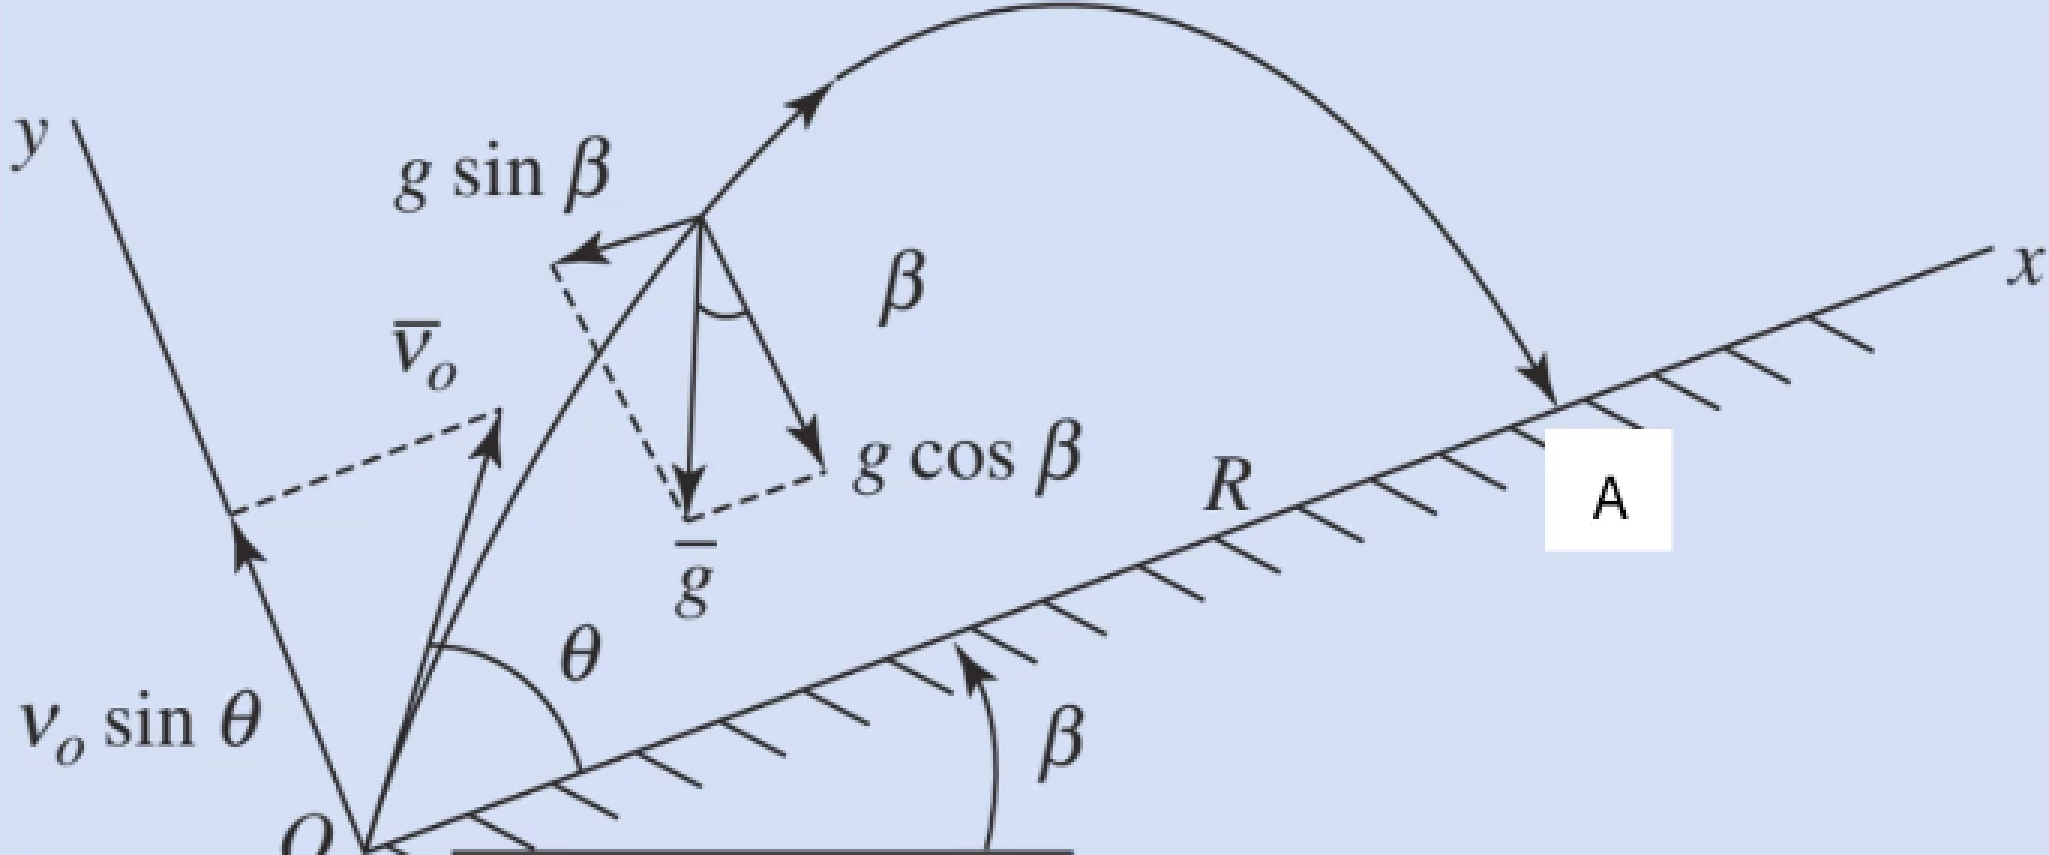
\includegraphics[width=0.5\textwidth]{db9.png}}
  \caption{Un proyectil sobre un plano inclinado}
  \label{db9}
\end{figure}

Es claro que en el aire, la trayectoria del proyectil es independiente del piso debajo. En cualquier punto, los componentes de la aceleración están dados por: 
\begin{equation}
    a_x=-g\sin{(\beta)}\quad a_y=-g\cos{(\beta)}
\end{equation}

Donde $\beta$ es la inclinación del plano con la horizontal. Cuando un proyectil es lanzado con velocidad $v_0$ haciendo un ángulo $\theta$ con el plano inclinado, las componentes $x$ y $y$ de la velocidad inicial están dadas por $v_0\cos{(\theta)}$ y $v_0\sin{(\theta)}$ respectivamente. Así en el tiempo $t$ después del lanzamiento, la coordenada de posición del proyectil está dada por: 

\begin{align}
    &x=v_0\cos{(\theta)}t-\frac{1}{2}g\sin{(\beta)}t^2\\
    &y=v_0\sin{(\theta)}t-\frac{1}{2}g\cos{(\beta)}t^2
\end{align}

El máximo valor de $y$ es cuando $v_y=0$. Las componentes de velocidad están dadas por:

\begin{align}
    &v_x=v_0\cos{(\theta)}-g\sin{(\beta)}t\\
    &v_y=v_0\sin{(\theta)}-g\cos{(\beta)}t
\end{align}

Así, $y$ es máximo después del tiempo $t^{*}$ donde: 

\begin{equation}
    t^*=\frac{v_0\sin{(\theta)}}{g\cos{(\beta)}}
\end{equation}

Si el proyectil golpea el plano nuevamente después de un tiempo $T$ (tiempo de vuelo) en el punto  $A$

\begin{equation}
    x_A=v_0\cos{(\theta)}T-\frac{1}{2}g\sin{(\beta)}T^2\\
\end{equation}

Después del tiempo $T$ la coordenada $y$ llega a ser cero nuevamente

\begin{align}
    &y=v_0\sin{(\theta)}t-\frac{1}{2}g\cos{(\beta)}t^2\\
    &0=v_0\sin{(\theta)}T-\frac{1}{2}g\cos{(\beta)}T^2
\end{align}

\begin{align*}
    &0=\left(v_0\sin{(\theta)}T-\frac{1}{2}g\cos{(\beta)}T \right)T\\
    &0=v_0\sin{(\theta)}-\frac{1}{2}g\cos{(\beta)}T\\
    &t=\frac{2v_0\sin{(\theta)}}{g\cos{(\beta)}}\, \mid y=0\\
    &R=x_A=v_0\cos{(\theta)}T-\frac{1}{2}g\sin{(\beta)}T^2\\
    &R=v_0\cos{(\theta)}\left(\frac{2v_0\sin{(\theta)}}{g\cos{(\beta)}}\right)-\frac{1}{2}g\sin{(\beta)}\left(\frac{2v_0\sin{(\theta)}}{g\cos{(\beta)}}\right)^2\\
    &R=v_0^2\left(\frac{2\sin{(\theta)}\cos{(\theta)}}{g\cos{(\beta)}}\right)-\frac{2\sin{(\beta)}}{g\cos^2{(\beta)}}\left(v_0^2\sin^2{(\theta)}\right)\\
    &R=v_0^2\left(\frac{\sin{(2\theta)}}{g\cos{(\beta)}}\right)-\frac{2\sin{(\beta)}}{g\cos^2{(\beta)}}\left(v_0^2\sin^2{(\theta)}\right)\\
    &R=\frac{v_0^2}{g\cos{(\theta)}}\left(\sin{(2\theta)}-2\tan{(\beta)}\beta\sin^2{(\theta)}\right)
\end{align*}

\begin{figure}[h!]
  \centerline{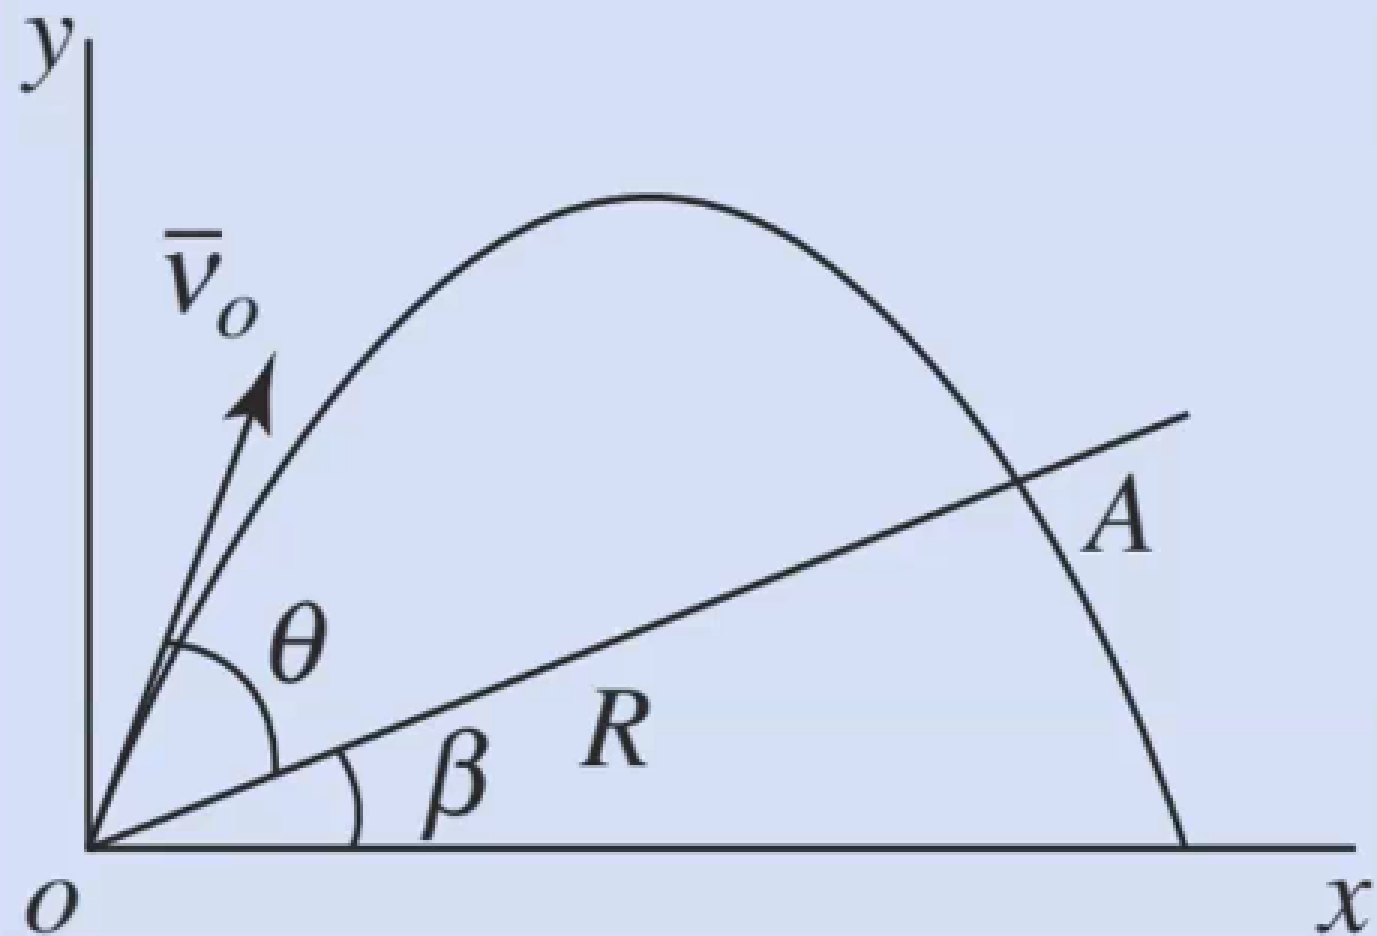
\includegraphics[width=0.5 \textwidth]{db10.png}}
  \caption{Usando el sistema de coordenadas $x-y$ en la dirección horizontal y vertical}
  \label{db10}
\end{figure}


\begin{align*}
    &x_A=v_0\cos{(\theta+\beta)}T\\
    &y_A=v_0\sin{(\theta+\beta)}T-\frac{1}{2}gT^2
\end{align*}

Ahora $\frac{y_A}{x_a}=\tan{(\beta)}$

\begin{align*}
    &\tan{(\beta)}=-\frac{y_a}{x_a}=\frac{v_0\sin{(\theta+\beta)}-\frac{1}{2}gT^2}{v_0\cos{(\theta+\beta)}T}\\
    &\tan{(\beta)}=\tan{(\theta+\beta)}-\frac{gT}{2v_0\cos{(\theta+\beta)}}\\
    &T=\frac{2v_0\cos{(\theta+\beta)}}{g}\left(\tan{(\theta+\beta)}-\tan{(\beta)}\right)\\
    &T=\frac{2v_0\cos{(\theta+\beta)}}{g}\left(\frac{\sin{(\theta+\beta)}}{\cos{(\theta+\beta)}}-\frac{\sin{(\beta)}}{\cos{(\theta)}}\right)\\
    &T=\frac{2v_0\cos{(\theta+\beta)}}{g}\left(\frac{\sin{(\cos{\beta})}\sin{(\theta+\beta)}-\sin{(\beta)}\cos{(\theta+\beta)}}{\cos{(\theta+\beta)}\cos{(\beta)}} \right)\\
    &T=\frac{2v_0\cos{(\theta+\beta)}}{g\cos{(\beta)}}\left(\cos{(\beta)}\sin{(\theta+\beta)}-\sin{(\beta)}\cos{(\theta+\beta)}\right)
\end{align*}
Reduciendo la expresión entre paréntesis

\begin{align*}
    &\cos{(\beta)}\sin{(\theta+\beta)}-\sin{(\beta)}\cos{(\theta+\beta)}=\\
    &\cos{(\beta)}\sin{(\theta)}\sin{(\beta)}+\cos{(\theta)}\sin{(\beta)}-\sin{(\beta)}\cos{(\theta)}\cos{(\beta)}+\sin{(\beta)}\sin{(\theta)}\sin{(\beta)}=\\
    &\sin{(\theta)}\left(\cos^2{(\beta)}+\sin^2{(\beta)}\right)=\sin{(\theta)}
\end{align*}
Entonces
\begin{equation*}
    T=\frac{2v_0}{g\cos{(\beta)}}\left(\sin{(\theta)}\right)
\end{equation*}

Tiempo de vuelo (tiempo desde el origen O hasta alcanzar el punto A)

\begin{equation}
    T=\frac{2v_0\sin{(\theta)}}{g\cos{(\beta)}}
\end{equation}

Distancia $R$
\begin{align}
    &x_a=R\cos{(\beta)}\\
    &y_A=R\sin{(\beta)}
\end{align}
De las ecuaciones de posición
\begin{align*}
        &x_A=v_0\cos{(\theta+\beta)}\left(\frac{2v_0\sin{(\theta)}}{g\cos{(\beta)}}\right)\\
        &y_A=v_0\sin{(\theta+\beta)}\left(\frac{2v_0\sin{(\theta)}}{g\cos{(\beta)}}\right)-\frac{1}{2}g\left(\frac{2v_0\sin{(\theta)}}{g\cos{(\beta)}}\right)^2\\
\end{align*}
\begin{align*}
    &R\cos{(\beta)}=v_0\cos{(\theta+\beta)}\left(\frac{2v_0\sin{(\theta)}}{g\cos{(\beta)}}\right)\\
    &R=\frac{2v_0^2}{g\cos^2{(\beta)}}\left(\sin{(2\theta+\beta)}-\sin{(\beta)}\right)
\end{align*}

\subsection{Movimiento curvilíneo:componentes normal y tangencial}

Cuando se conoce la trayectoria a lo largo de la cual viaja a una partícula, resulta conveniente describir el movimiento por medio de los ejes coordenados $n$ y $t$ a lo largo de la normal y tangente a la trayectoria, respectivamente.

Movimiento en el plano. Considere una partícula que se desplaza en un plano a lo largo de una curva fija. Considere un sistema de coordenadas que tiene su origen sobre la curva, y en el instante considerado este origen coincide con la ubicación de la partícula. El eje $t$ es tangente a la curva en el punto y es positivo en la dirección de $s$ creciente. El eje normal $n$ es perpendicular al eje $t$ con su sentido positivo dirigido hacia el centro de curvatura $O^{\prime}$

de la figura, $ds=\rho \,d\theta$ dividiendo por $dt$ se obtiene $\dot{s}=\rho\dot{\theta}$

\begin{wrapfigure}{l}{0.25\textwidth}
  \centerline{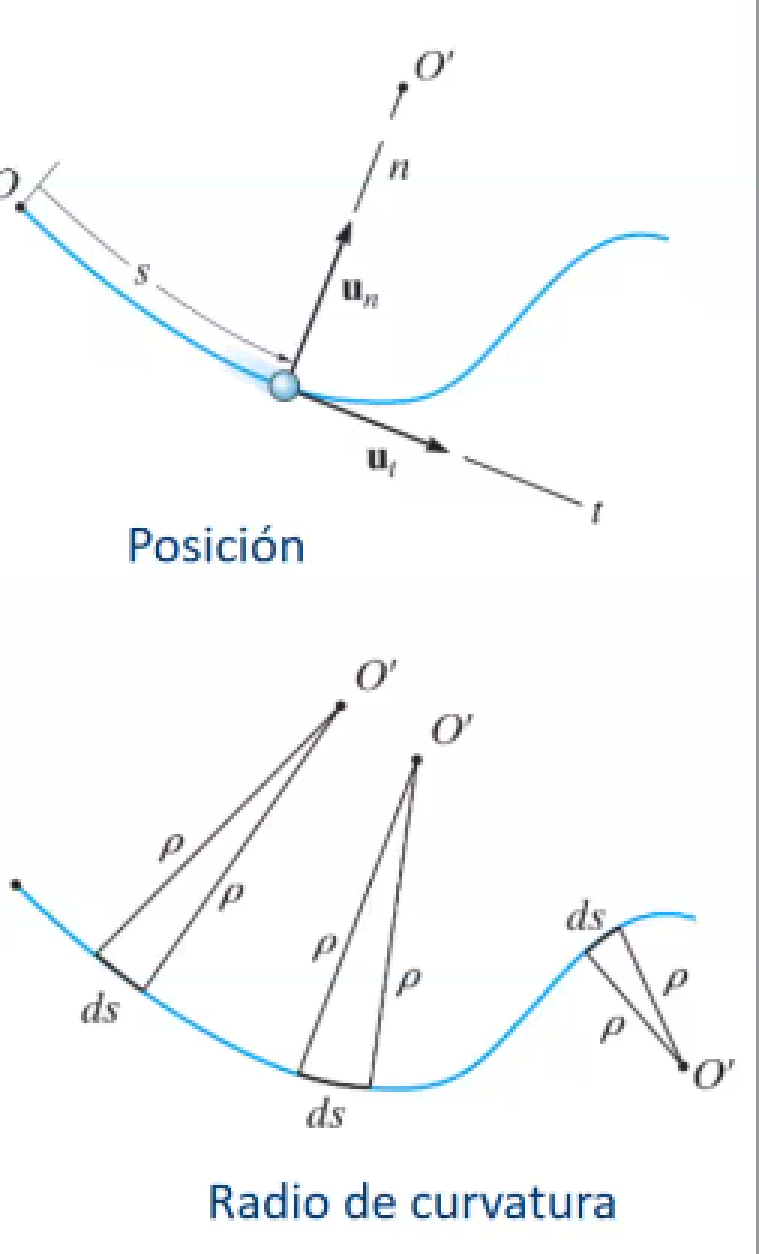
\includegraphics[width=0.5\textwidth]{db11.png}}
  \caption{Movimiento curvilínea, posición y radio de curvatura}
  \label{db11}
\end{wrapfigure}


Velocidad. La dirección de la velocidad $v$ de la partícula siempre es tangente a la trayectoria y su magnitud se determina por $d=\frac{ds}{dt}$

\begin{equation}
    v=vu_t
\end{equation}

donde $V=\dot{s}$

Aceleración. Es la razón de cambio de la velocidad con respecto al tiempo

\begin{equation}
    a=\dot{V}=\dot{v}u_t+v\dot{u}_t
\end{equation}

Pero el radio de curvatura se tiene: 

\begin{equation}
    \dot{u}_t=u_n\frac{1}{\rho}\dot{s}=\frac{v}{\rho}u_n
\end{equation}

\begin{figure}[h!]
  \centerline{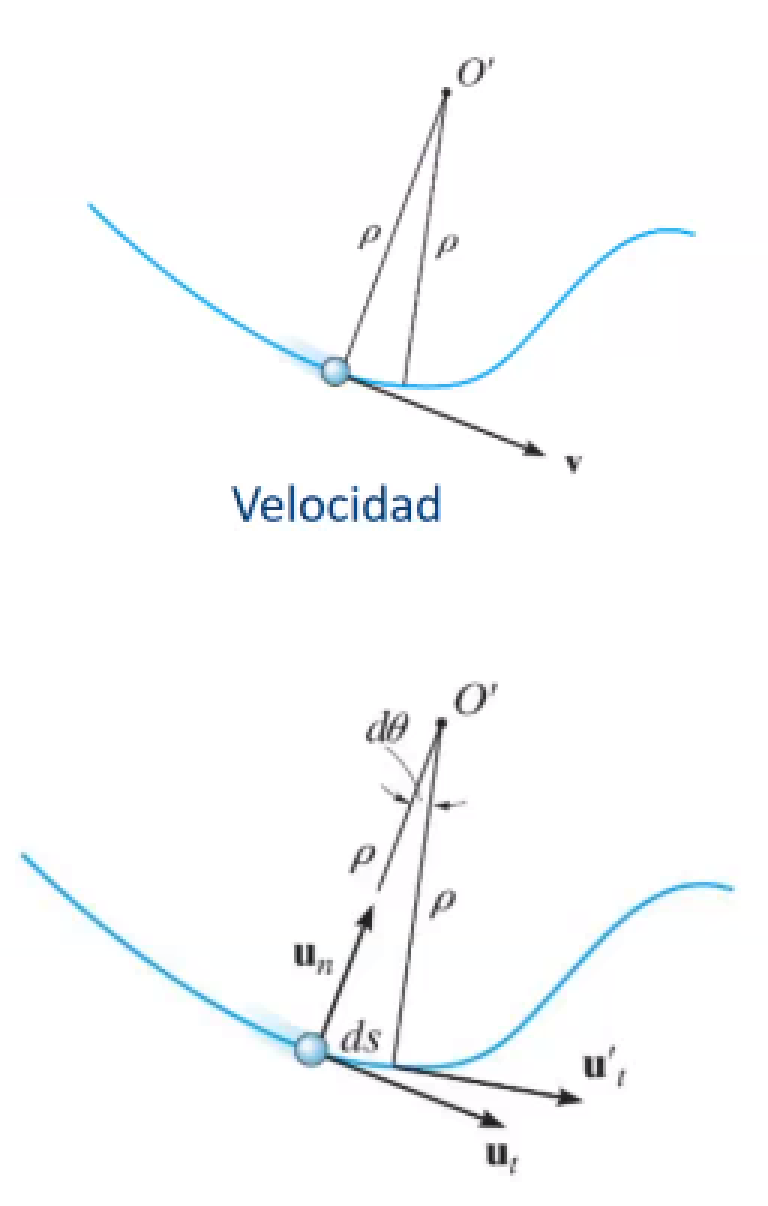
\includegraphics[width=0.5\textwidth]{db12.png}}
  \caption{Velocidad}
  \label{db12}
\end{figure}

Al sustituir en la ecuación de la aceleración $A$:
\begin{equation}
    A=a_tu_t+a_nu_m
\end{equation}
donde $a_t=\dot{v}$ o $a\,ds=v\,dv$ y $a_n=\frac{v^2}{\rho}$

La magnitud de la aceleración es el valor positivo de:
\begin{equation}
    a=\sqrt{a_t^2+a_n^2}
\end{equation}

Si la ecuación de la trayectoria es conocida, el radio de curvatura se calcula con:
\begin{equation*}
    \rho=\frac{\left[1+\left(\frac{dy}{dx}\right)^2\right]^{\frac{3}{2}}}{\left(\frac{d^2y}{dx^2}\right)}=\frac{\left[1+\left(\frac{dx}{dy}\right)^2\right]^{\frac{3}{2}}}{\left(\frac{d^2x}{dy^2}\right)}
\end{equation*}

\begin{figure}[h!]
  \centerline{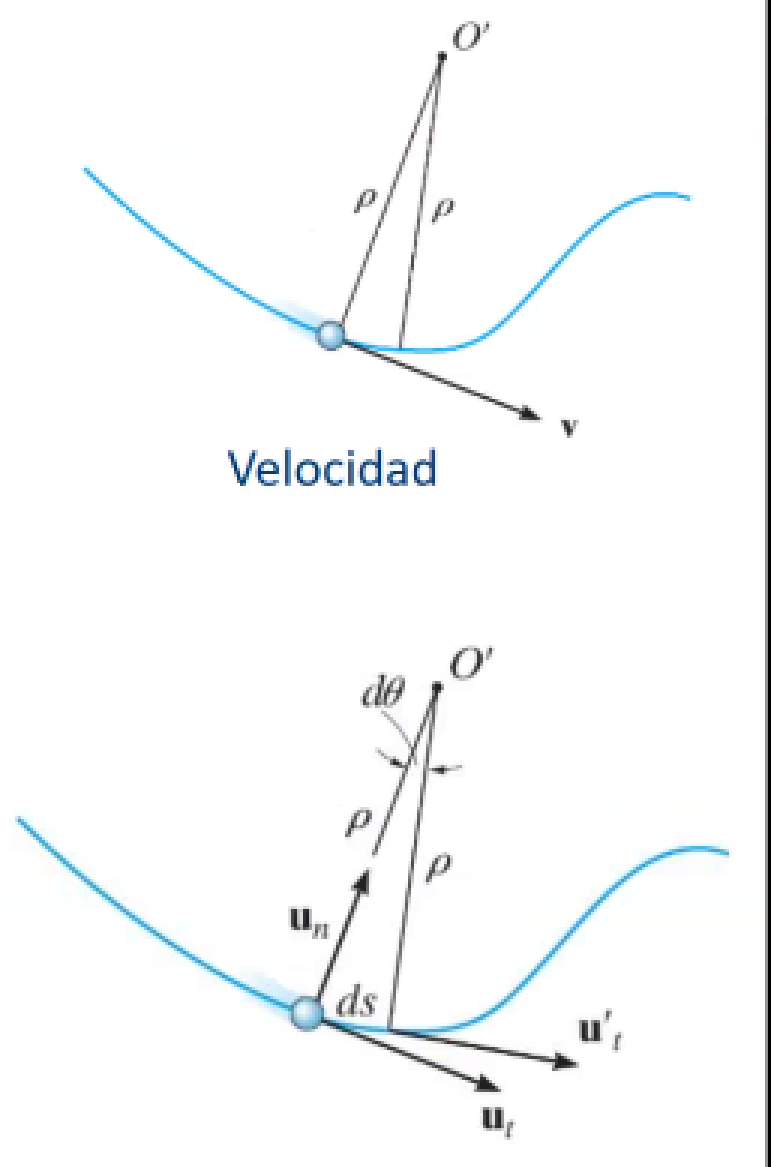
\includegraphics[width=0.5\textwidth]{db13.png}}
  \caption{Aceleración}
  \label{db13}
\end{figure}

Casos especiales de movimiento:

\begin{itemize}
    \item Si la partícula se mueve en línea recta, $\rho\to\infty$ y $a_n=0$ por tanto $a=a_t=\dot{v}$
    la componente tangencial de la aceleración representa la razón de cambio con respecto al tiempo en la magnitud de la velocidad
    \item Si la partícula se mueve a lo largo de una curva con rapidez constante $a_t=\dot{v}=0$ y $a=a_n=\frac{v^2}{\rho}$. La componente normal de la aceleración representa la razón de cambio con respecto al tiempo en la dirección de la velocidad
\end{itemize}

\begin{figure}[h!]
  \centerline{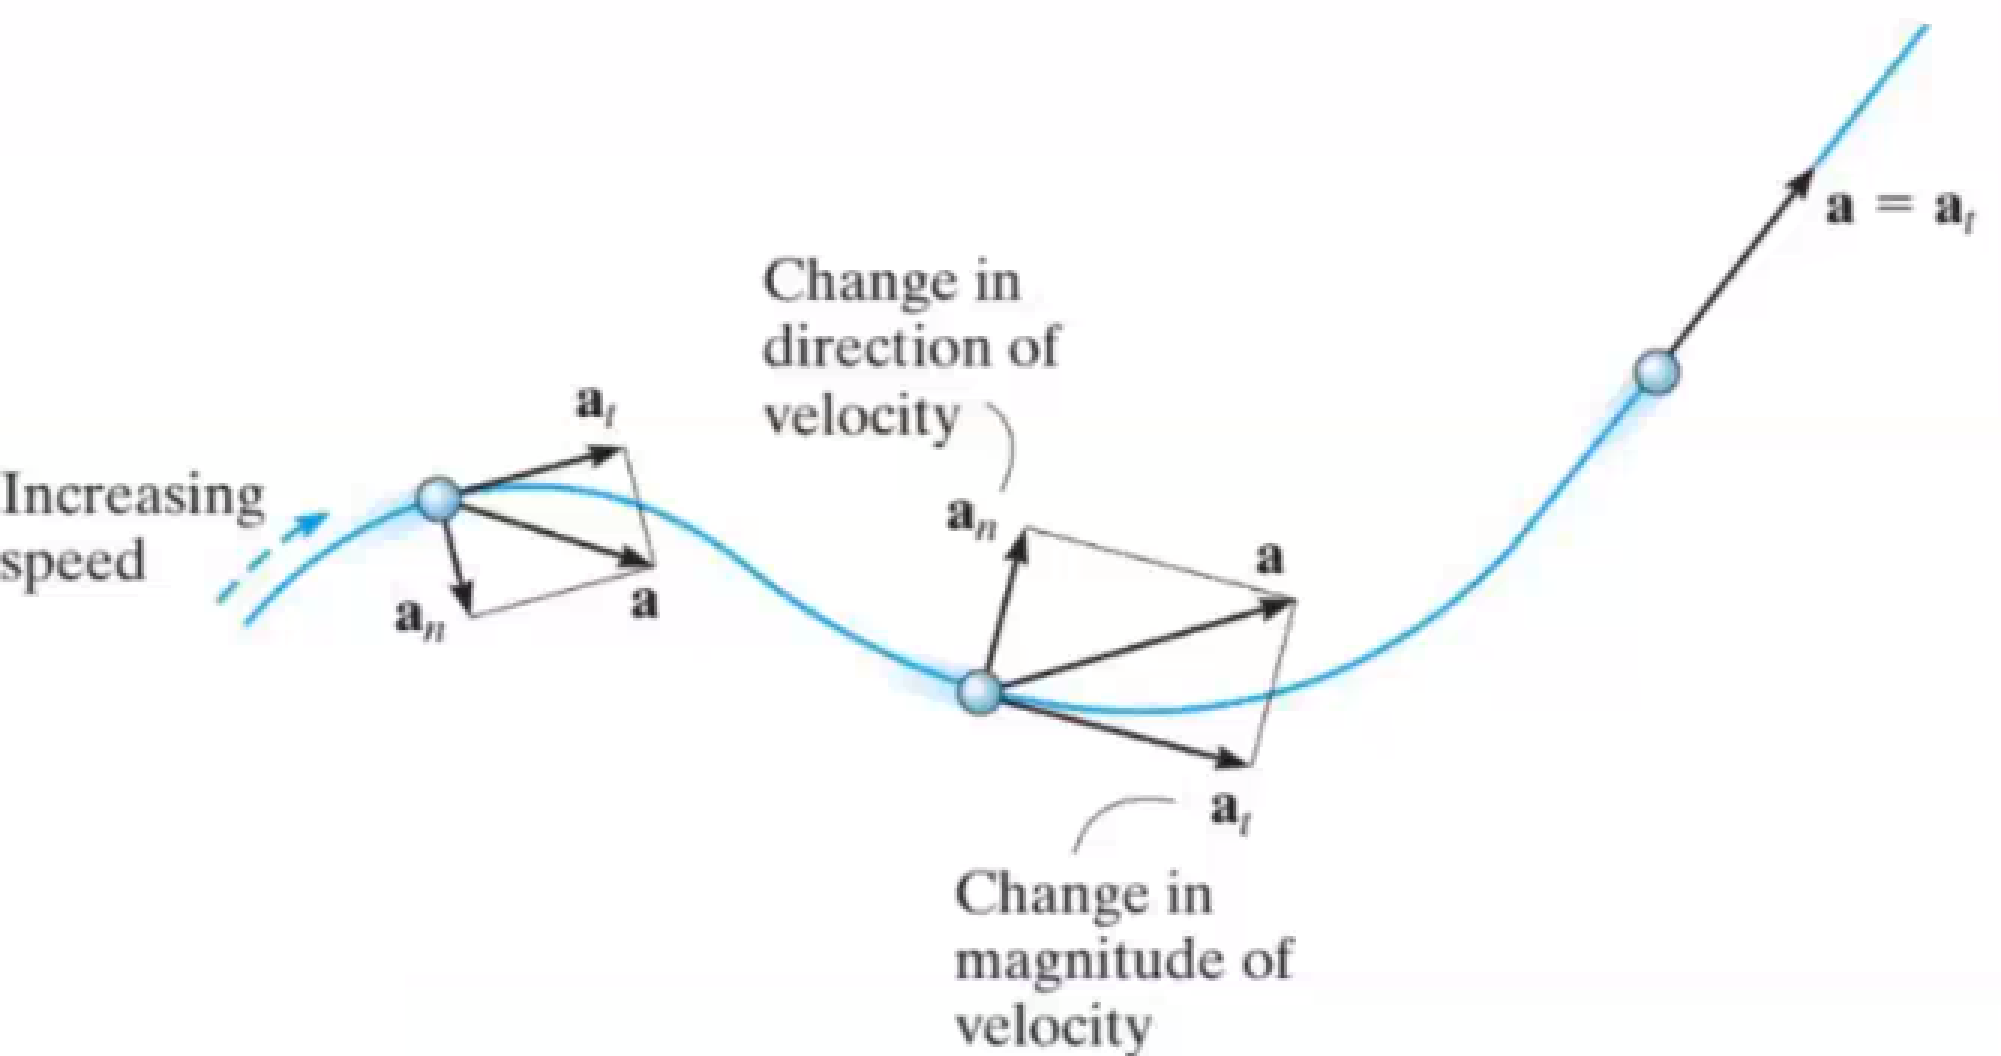
\includegraphics[width=0.5\textwidth]{db14.png}}
  \caption{Componentes normal y tangencial}
  \label{db14}
\end{figure}

\begin{example}
    Cuando el esquiador llega al punto $A$ a lo largo de la trayectoria parabólica, su rapidez es de 8m/s, la cual se incrementa a $2m/s^2$. Determine la dirección de su velocidad y la dirección y magnitud de su aceleración en este instante. Al hacer los cálculos, desprecie la estatura del esquiador.
\end{example}

\textit{ Sol. }

La velocidad es tangente a la trayectoria.

\begin{align*}
    &y=\frac{1}{20}x^2\implies \frac{dy}{dx}=\frac{1}{10}x\\
    &x=10,\implies \frac{dy}{dx}=1
\end{align*}

V forma un ángulo $\theta=\arctan{(1)}=45^{\circ}$ y $v_a=8m/s$ con $\theta=45^{\circ}$

Aceleración: cuando $\dot{v}=2m/s$. Radio de curvatura cuando $x=10$: $\frac{dy}{dx}=1,\frac{d^2y}{d x^2}=\frac{1}{10}$

\begin{align*}
    &\rho=\frac{\left[1+(1)^2\right]^{3/2}}{\frac{1}{10}}=28.28\\
    &a=(2)u_t+\frac{(8m/s)^2}{28.28}u_n\, a=(2u_+2.26u_n)m/s^2 \\ 
    &a=\sqrt{\left(2m/s^2\right)^2+\left(2.26m/s^2\right)^2}=3.02m/s^2\\
    &\phi=\arctan{\frac{2.26m/s^2}{2m/s^2}}=\frac{\pi}{4}=\frac{2}{2.26}=41.5^{\circ}\\
    &180^{\circ}- 45^{\circ} +90^{\circ}+41.5^{\circ}=3.5^{\circ}\\
    &a=3.02m/s^2\, 3.5^{\circ}
\end{align*}

\subsection{Movimiento curvilíneo: Componentes Cilíndricos}

\begin{definition}[Coordenadas polares]
    La ubicación de la partícula se específica con una coordenada radial $r$ y una coordenada transversal $\theta$. Los vectores unitarios $u_r$ y $u_{\theta}$ definen las direcciones positivas de las coordenadas $r$ y $\theta$, respectivamente. Estas direcciones son perpendiculares entre sí.
\end{definition}

\begin{figure}[h!]
  \centerline{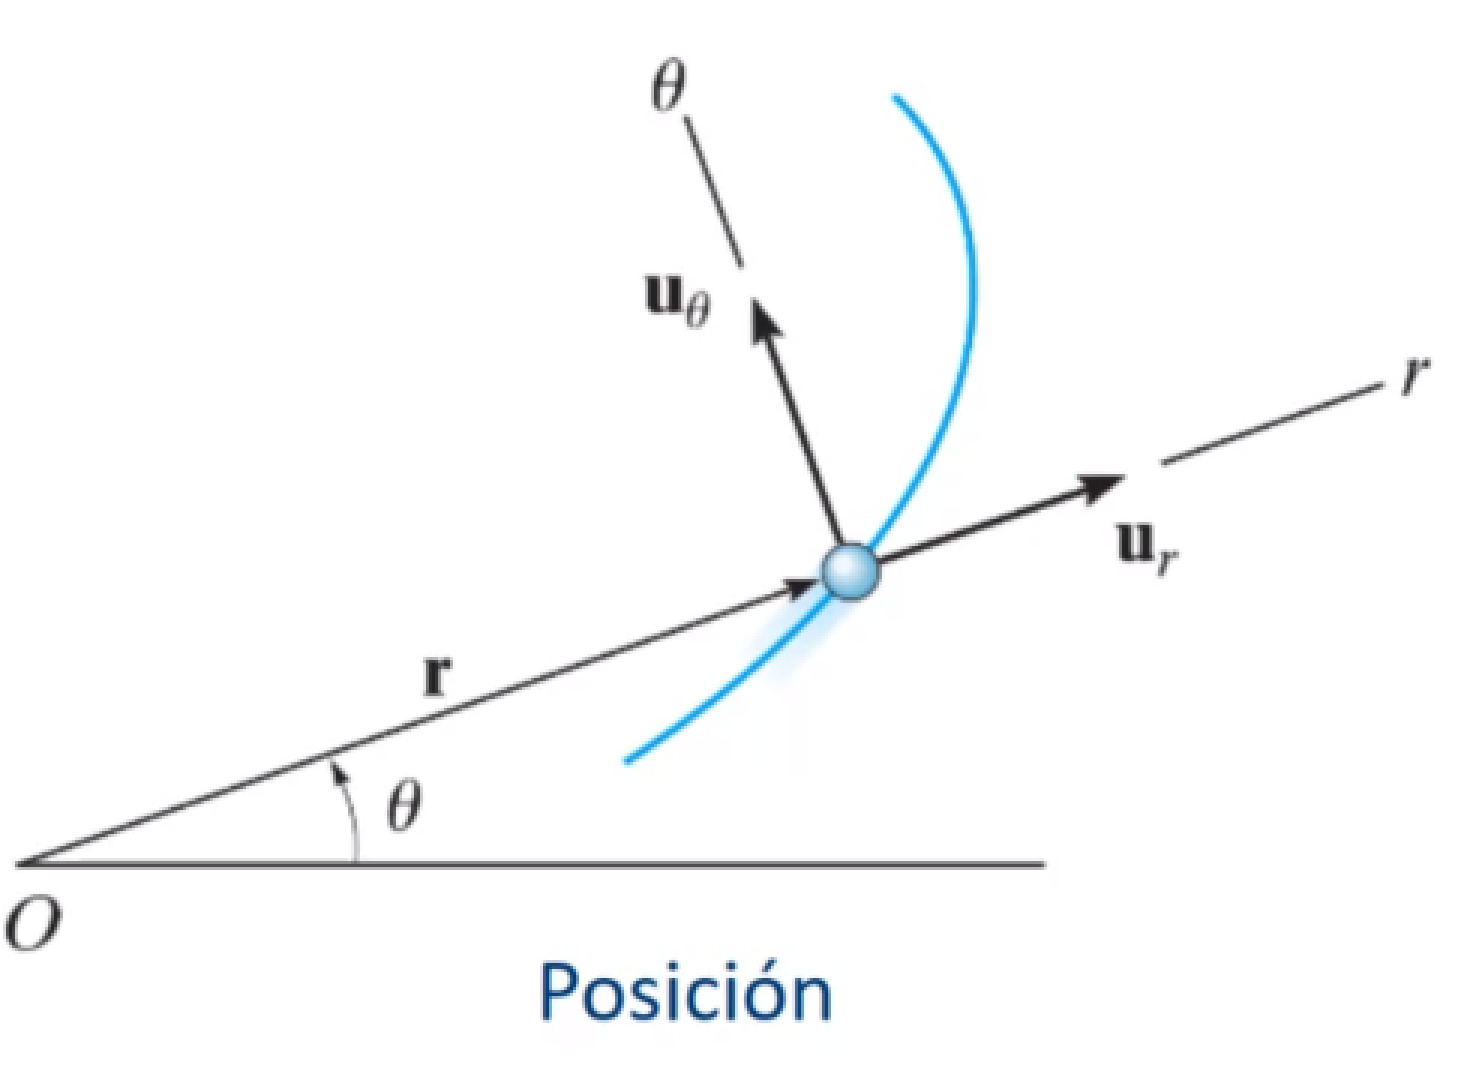
\includegraphics[width=0.5\textwidth]{db16.png}}
  \caption{Movimiento curvilíneo}
  \label{db16}
\end{figure}

\begin{definition}[Posición]
    La posición de la partícula está definida por el vector de posición 
    \begin{equation}
        R=ru_r
    \end{equation}
\end{definition}

\begin{definition}[Velocidad]
    La velocidad instantánea $v$ se obtiene al tomar la derivada con respecto al tiempo de r
    \begin{equation}
        v=\dot{r}=\dot{r}u_r+r\dot{u}_r
    \end{equation}
\end{definition}

Las derivadas temporales de los vectores $u_r$ y $u_{\theta}$ se obtienen al tomar la derivada con respecto al tiempo de $r$ y $\theta$ pueden determinarse relacionando los vectores con el sistema de coordenadas $xy$. De la figura del vector de posición

\begin{figure}[h!]
  \centerline{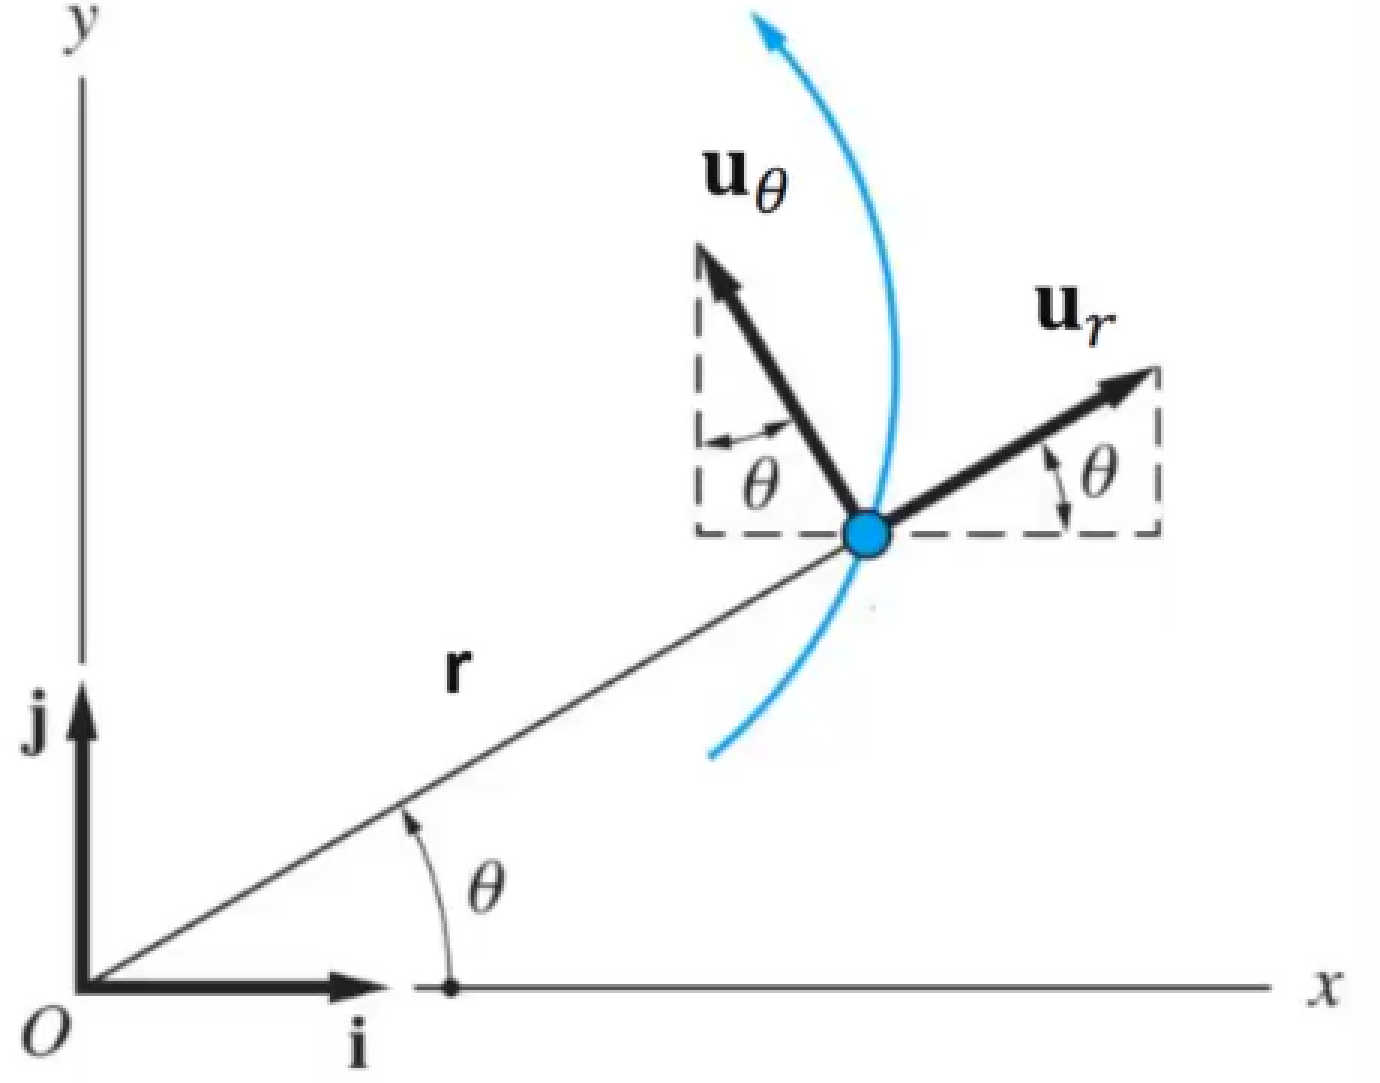
\includegraphics[width=.05\textwidth]{db17.png}}
  \caption{Componentes polares}
  \label{db17}
\end{figure}

\begin{align}
    &u_r=\cos{(\theta i)}+\sin{(\theta i)}\\
    &u_{\theta}=-\sin{(\theta i)}+\cos{(\theta i)}
\end{align}
Al derivar con respecto al tiempo $di/dt=dj/dt=0$ el marco $xy$ es fijo.
\begin{align*}
    &\frac{du_r}{dt}=\left(-\sin{(\theta i)}+\cos{(\theta j)}\right)\dot{\theta}\\
    &\frac{du_{\theta}}{dt}=\left(-\cos{(\theta i)}-\sin{(\theta j)}\right)\dot{\theta}
\end{align*}
\begin{align*}
\dot{u}_r=\dot{\theta}&u_{\theta}=-\dot{\theta}_r
\end{align*}
La variable $\dot{\theta}$ es la velocidad angular de la línea radial. Los vectores $\dot{u}_r$ y $\dot{u}_{\theta}$ son perpendiculares a $u_r$ y $u_{\theta}$ respectivamente.

Sustituyendo este resultado en la ecuación: 
\begin{equation*}
    v=\dot{r}+\dot{r}u_r+r\dot{u}_r
\end{equation*}

La velocidad se escribe en su forma de componentes como
\begin{equation*}
    v=v_ru_r+v_{\theta}u_{\theta}
\end{equation*}
donde: 
$v_r=\dot{r}$ es el componente radial y $v_{\theta}=r\dot{\theta}$ es la componente transversal

La magnitud de la velocidad o rapidez es el valor positivo de

\begin{equation}
    v=\sqrt{(\dot{r})^2+(r\dot{\theta})^2}
\end{equation}
y la dirección de $v$ es tangente a la trayectoria

\begin{figure}[h!]
  \centerline{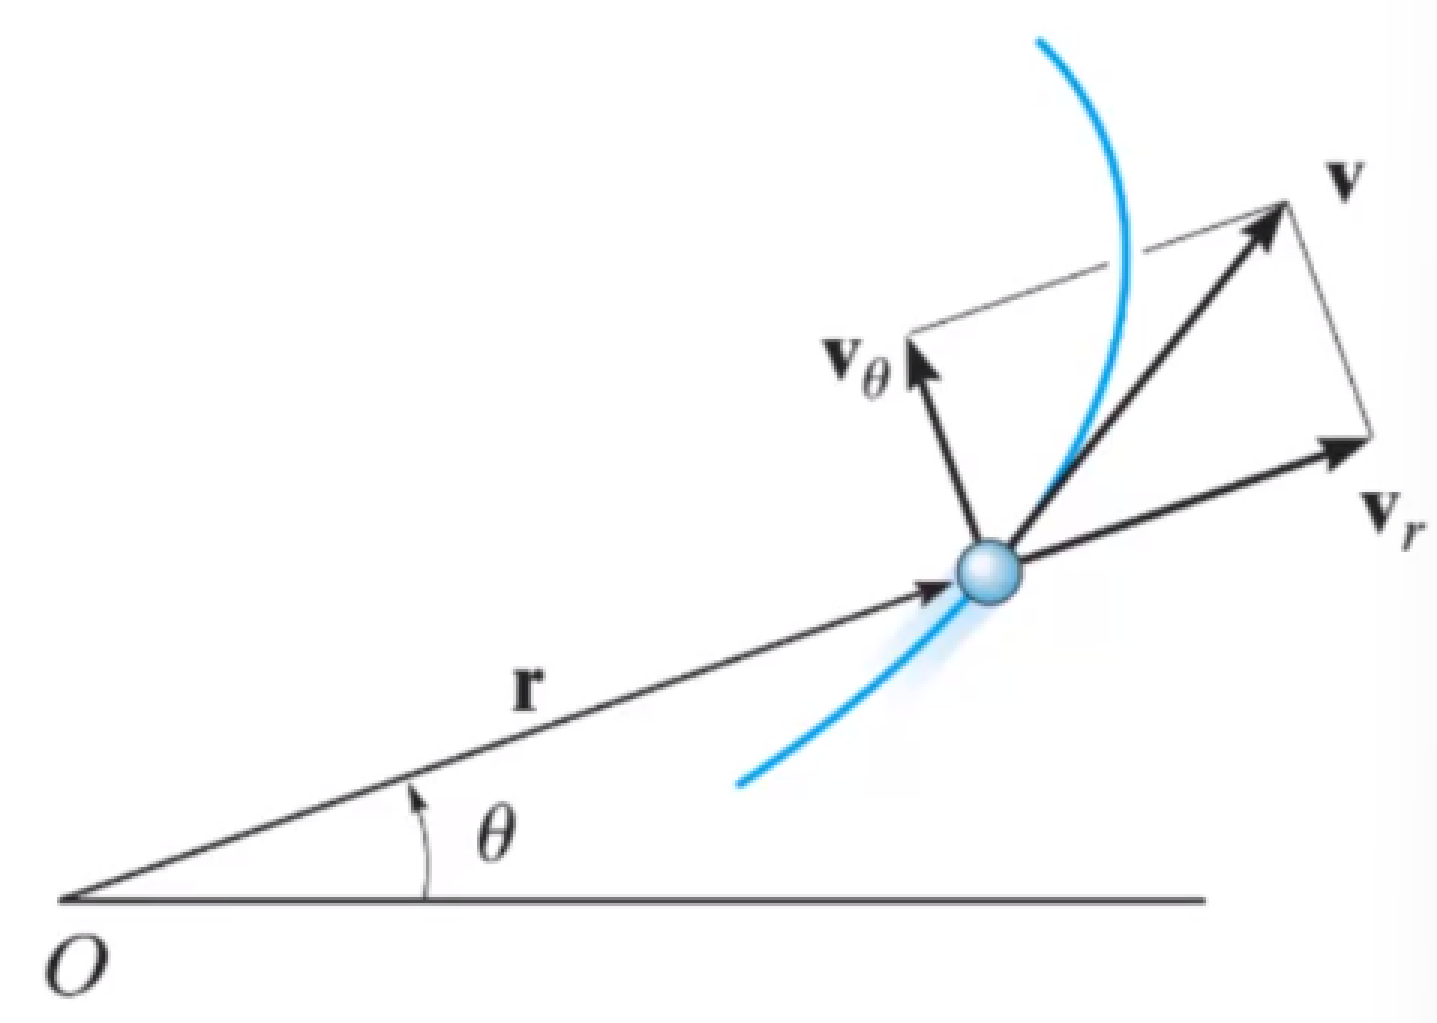
\includegraphics[width=0.5\textwidth]{db18.png}}
  \caption{Velocidad}
  \label{db18}
\end{figure}

Aceleración: El vector de velocidad se calcula como sigue

\begin{align*}
    &a=\frac{dv}{dt}=\frac{d}{dt}\left(\dot{r}u_r+r\dot{\theta}u_{\theta}\right)\\
    &a=\left(\ddot{r}+\dot{r}\dot{u}_r\right)+\left(\dot{r}\dot{\theta}u_{\theta}+r\ddot{\theta}u_{\theta}+r\dot{\theta}\dot{u}_{\theta}\right)
\end{align*}

La variable $\ddot{\theta}$ se llama aceleración angular de la recta radial. Sustituyendo $\dot{u}_{\theta}=-\dot{\theta}u_r$ en la ecuación para $a$, escribimos la aceleración en su forma de componentes como

\begin{equation}
    a=a_ru_r+a_{\theta}u_{\theta}
\end{equation}

donde $a_r=\ddot{r}-\dot{r}\dot{\theta}^2$ y $a_{\theta}=r\ddot{\theta}+2\dot{r}\dot{\theta}$

\begin{figure}[h!]
  \centerline{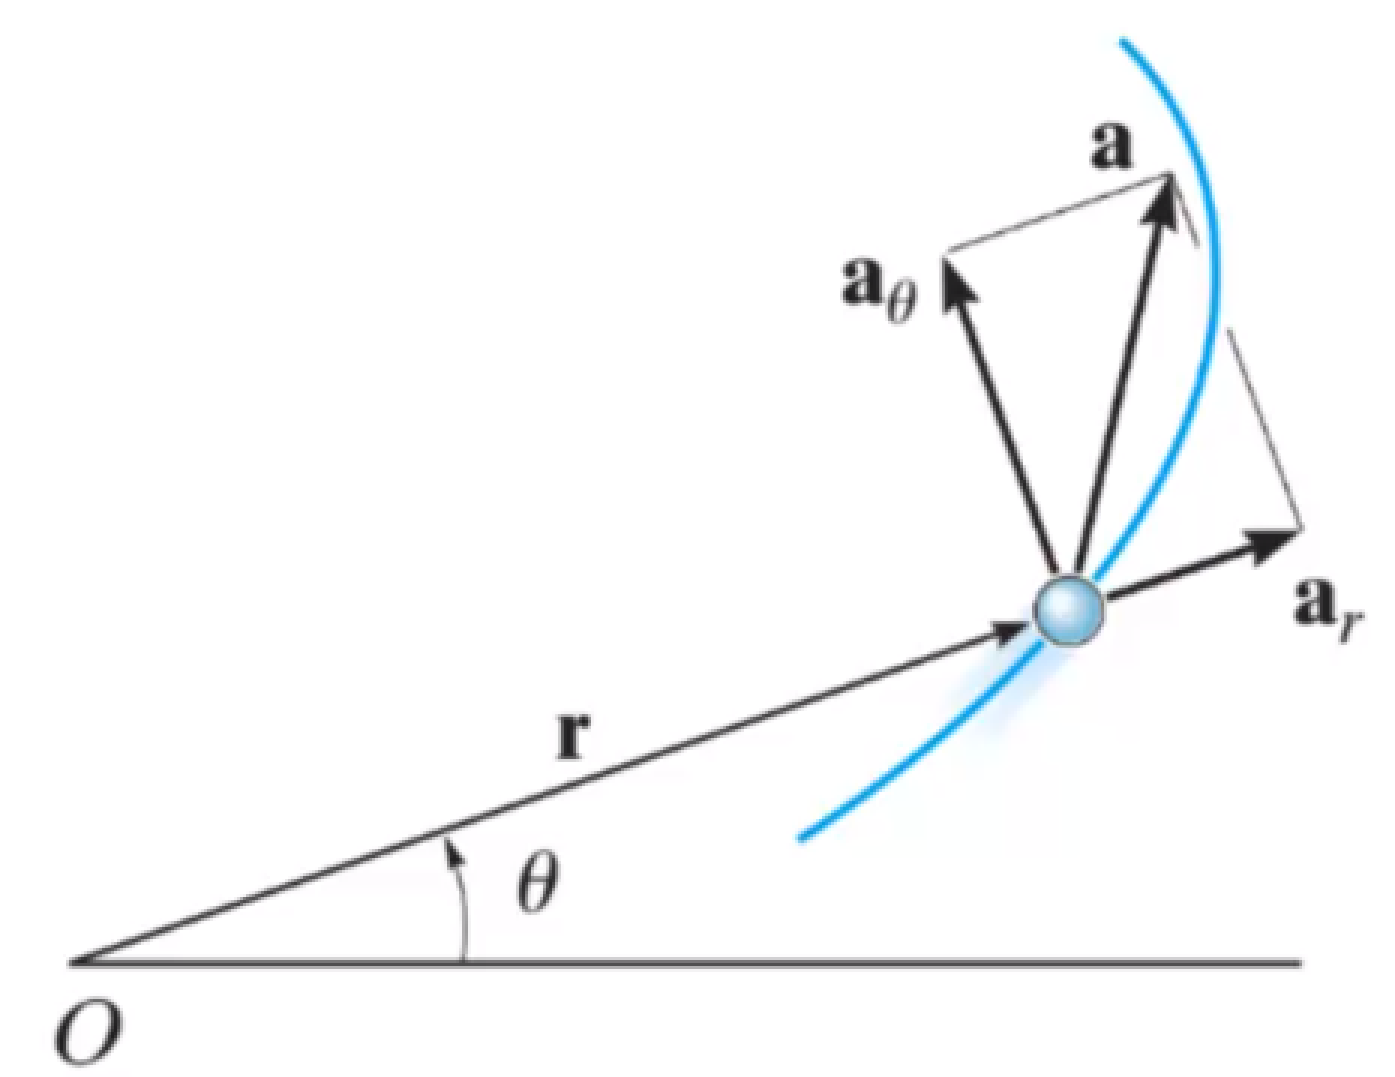
\includegraphics[width=0.5\textwidth]{db19.png}}
  \caption{Aceleración}
  \label{db19}
\end{figure}


\begin{definition}[Coordenadas cilíndricas]
    Si la partícula se mueve a lo largo de una curva espacial, entonces su ubicación se específica por medio de las tres coordenadas cilíndricas, $r$, $\theta$, $z$, posición, velocidad y aceleración:
\end{definition}

\begin{align}
    &r_p=ru_r+zu_z\\
    &v=\dot{r}u_r+r\dot{\theta}u_{\theta}+\dot{z}u_z\\
    &a=\left(\ddot{r}-r\dot{\theta}^2\right)u_r+\left(r\ddot{\theta}+2\dot{r}\dot{\theta}\right)u_{\theta}+\ddot{z}u_z
\end{align}

\begin{figure}[h!]
  \centerline{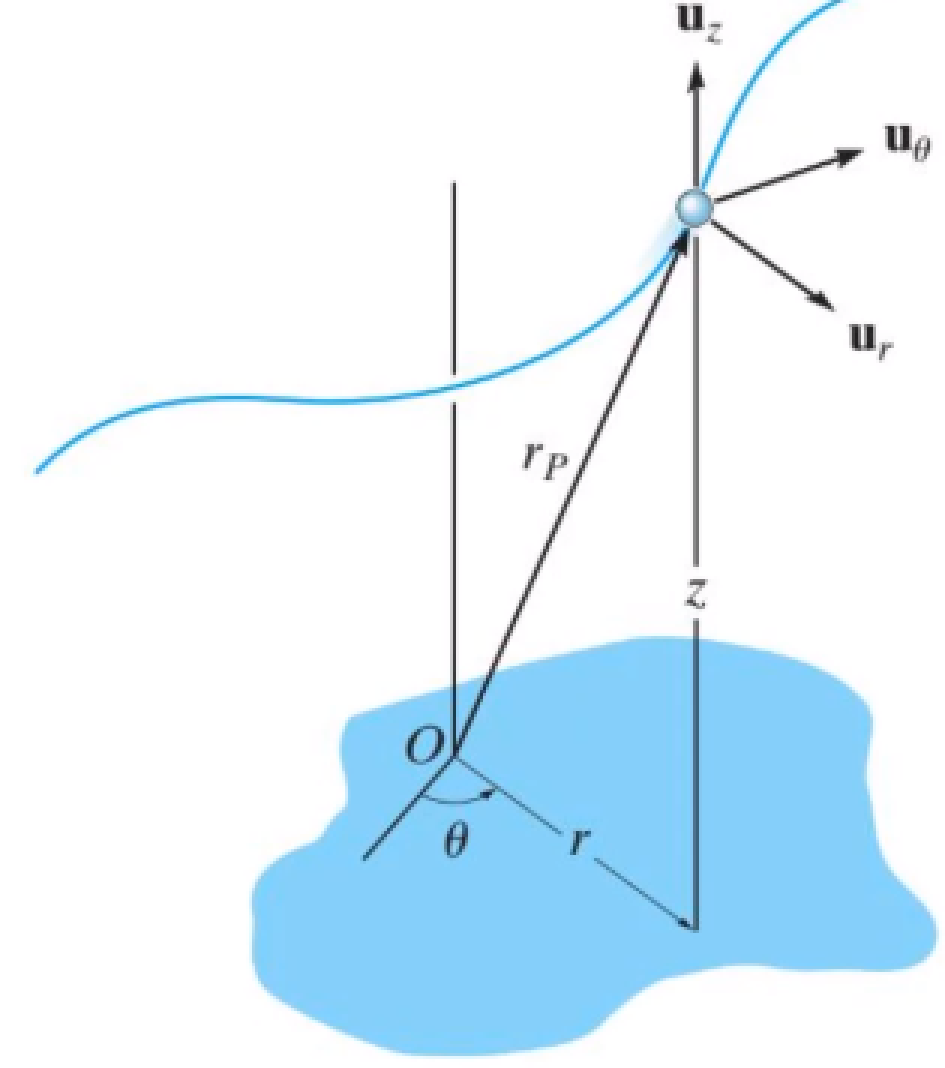
\includegraphics[width=0.5\textwidth]{db20.png}}
  \caption{Coordenadas cilíndricas}
  \label{db20}
\end{figure}

\begin{example}
    El cable conectado del torno $A$ al punto $B$ sobre el
carro de ferrocarril de la figura se enrolla con una razón constante de $2 m/s$. Cuando $\theta=60^{\circ}$ , determine: 
\begin{enumerate}
    \item la velocidad de $B$ y $\dot{\theta}$, y
    \item la aceleración de $B$ y $\ddot{\theta}$. Desprecie el radio del torno.
\end{enumerate}
\end{example}

\begin{figure}[h!]
  \centerline{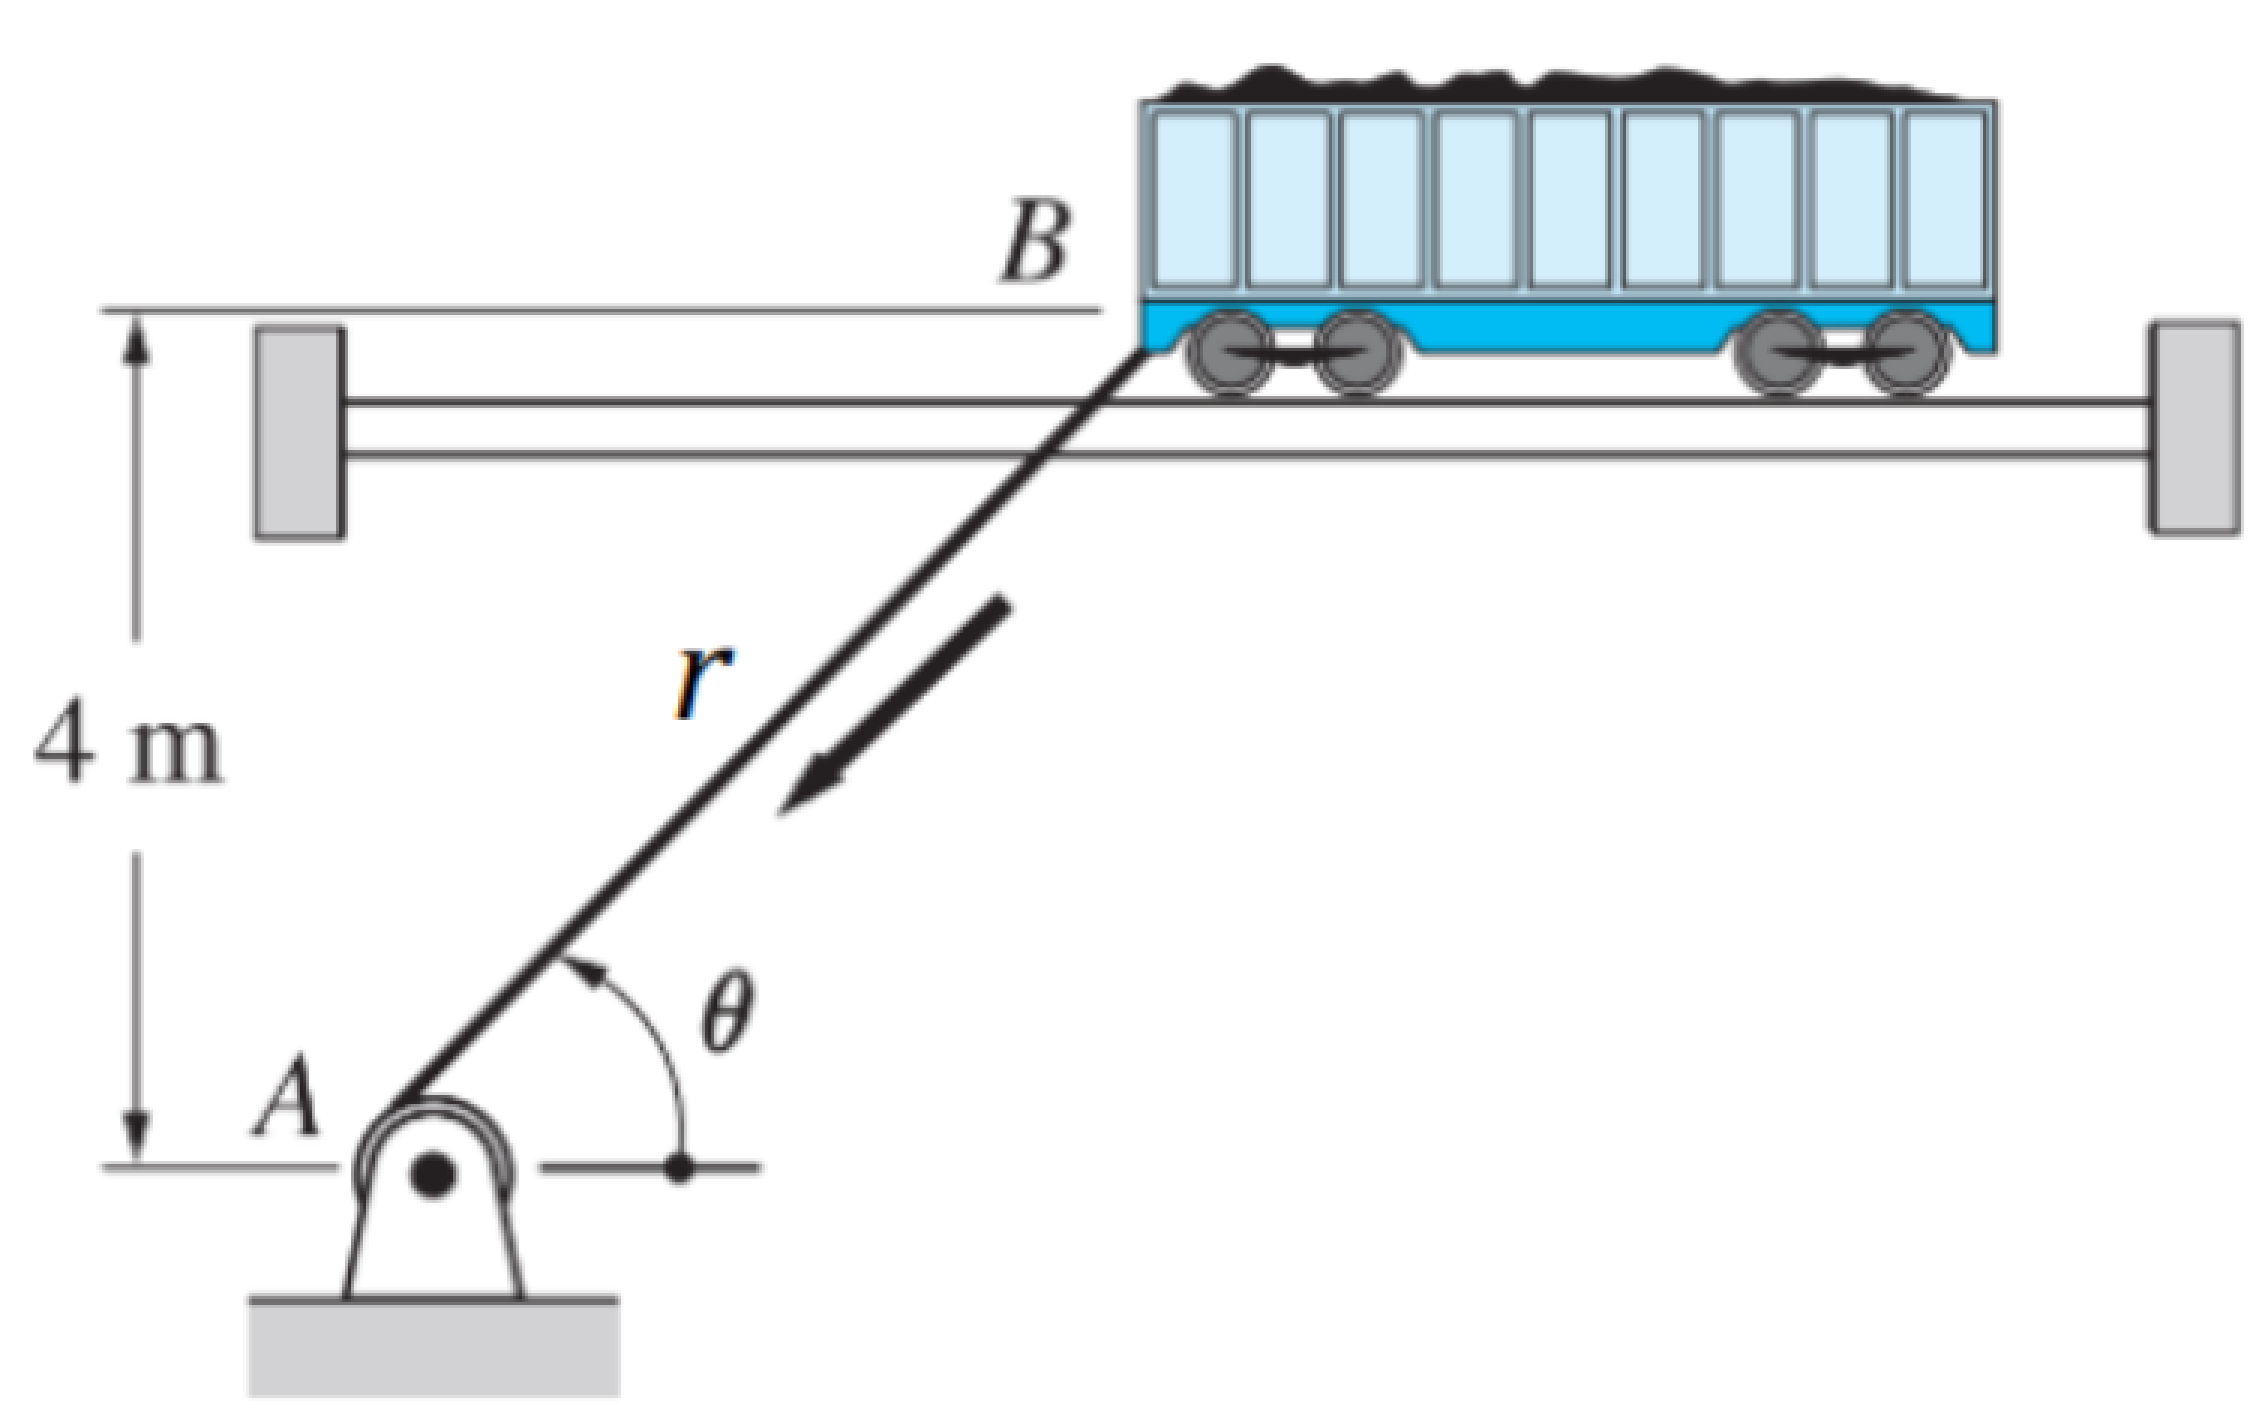
\includegraphics[width=0.5\textwidth]{db21.png}}
  \caption{Esquema del problema}
  \label{db21}
\end{figure}

\textit{ Sol. }

En la figura se observa que la longitud $R$ del cable y el
ángulo $\theta$ son las coordenadas polares del punto $B$. En $\theta=60^{\circ}$, se tiene:
\begin{equation*}
    R=\frac{4}{\sin{\theta}}=\frac{4}{\sin{\theta}}=4.619m
\end{equation*}

De acuerdo al enunciado del problema, R se reduce a razón
constante de $2 m/s$. Por tanto

\begin{align*}
    &\dot{R} = -2 m/s &&\ddot{R}= 0 m/s^2
\end{align*}

El punto B sigue una trayectoria recta horizontal, en
consecuencia, sus vectores velocidad y aceleración
también son horizontales.

\begin{figure}[h!]
    \centerline{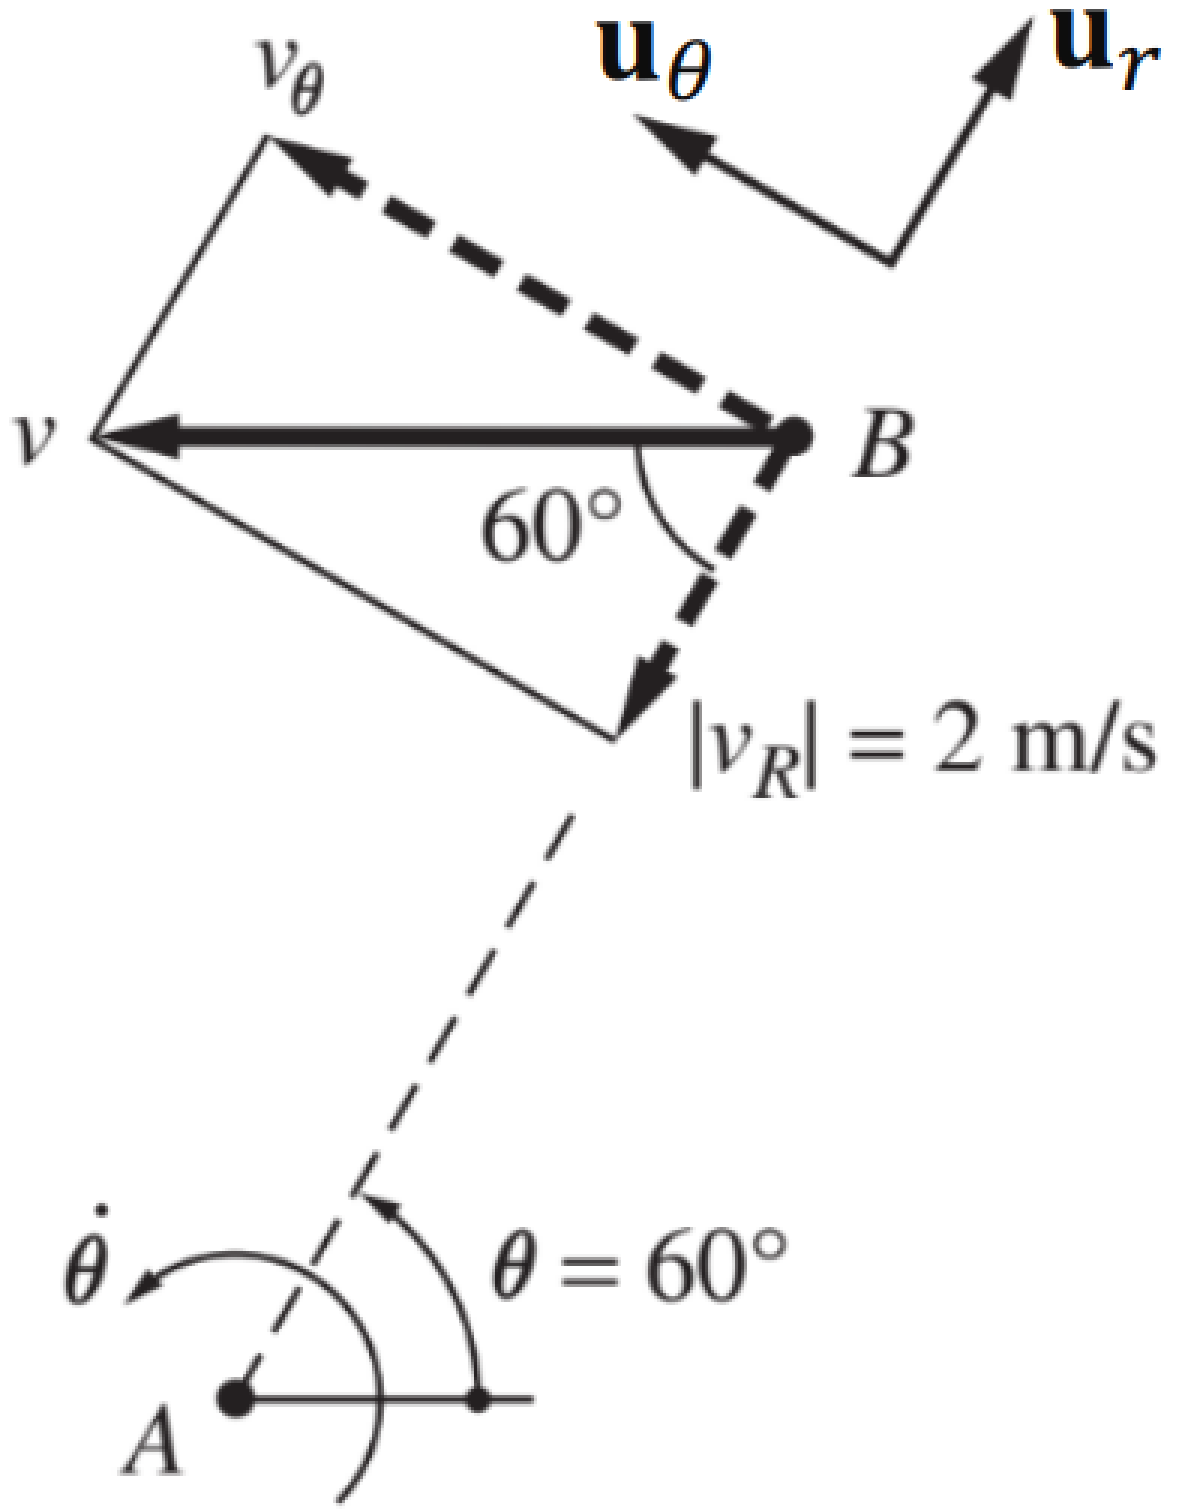
\includegraphics[width=0.5\textwidth]{db22.png}}
    \caption{descomposición del vector de velocidad $v$ de $B$,}
    \label{db22}
  \end{figure}

La figura \ref{db22} muestra la descomposición del vector de
velocidad $v$ de $B$, en sus componentes radial y transversal,
$\theta = 60^{\circ}$. De la geometría de diagrama, la rapidez de $B$ en
$\theta = 60^{\circ}$ es
\begin{equation*}
    v=\frac{2}{\cos{(60^{\circ})}}
\end{equation*}
El diagrama de velocidad también da $v_{\theta}=2\tan{60^{\circ}}$.
Comparando este resultado con $v_{\theta} = R\dot{\theta}$, encontramos
que:
\begin{equation*}
    \dot{\theta}=\frac{v_{\theta}}{R}=\frac{2\tan{(60^{\circ})}}{4.619}=0.75rad/s
\end{equation*}

\begin{figure}[h!]
  \centerline{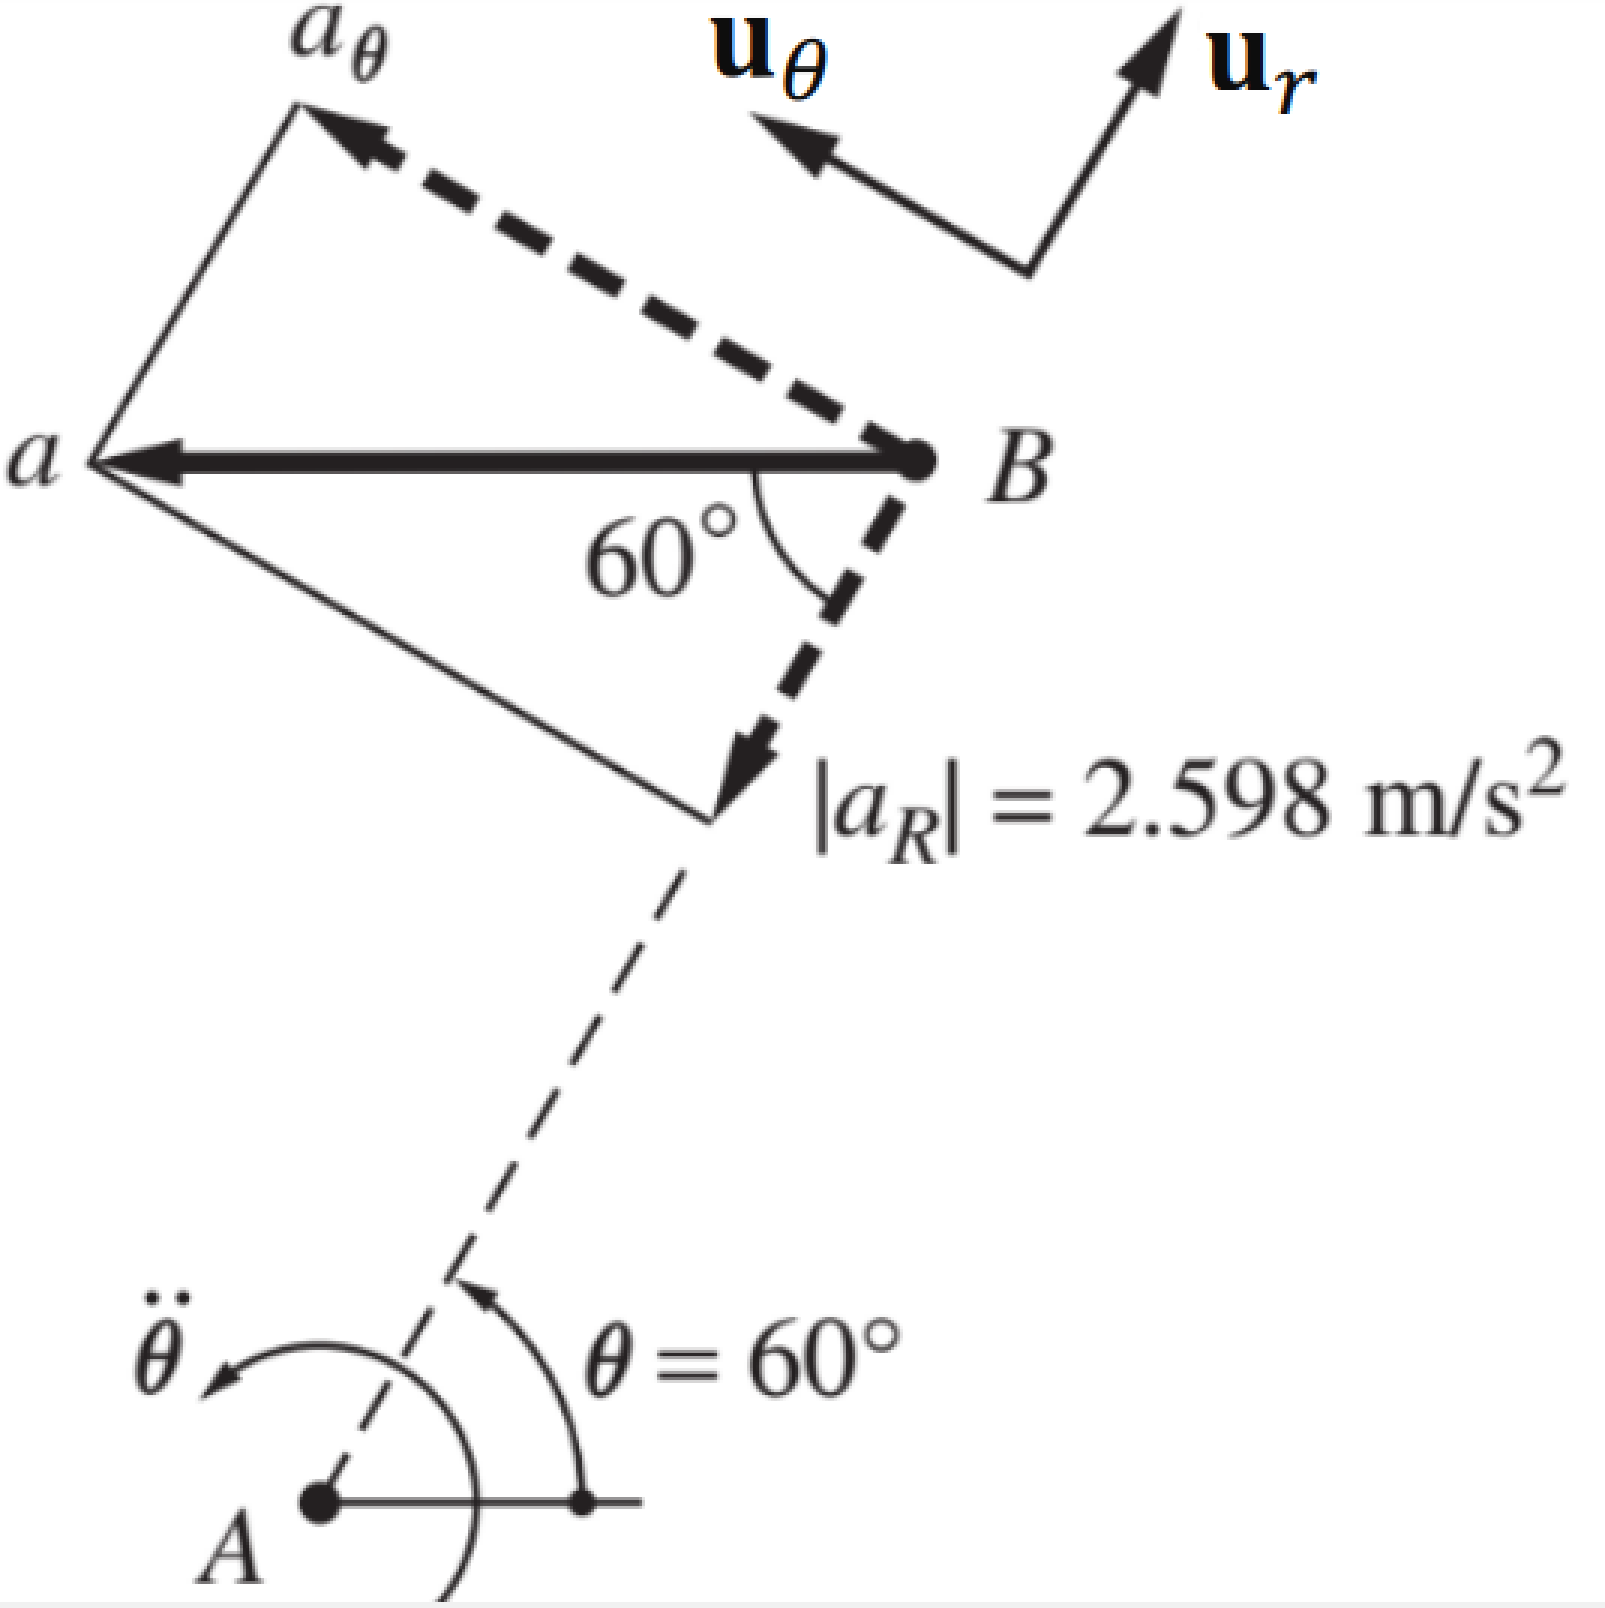
\includegraphics[width=0.5\textwidth]{db23.png}}
  \caption{Aceleración radial}
  \label{db23}
\end{figure}
En la figura \ref{db23} se muestra el diagrama de aceleración de un
punto B en $\theta = 60^{\circ}$. La componente radial es:
\begin{equation*}
    a_r=\ddot{r}-r\dot{\theta}^2=0-(4.619)(0.75)^2=-2.598m/s^2
\end{equation*}
Se sabe que el vector velocidad es horizontal, entonces es
posible completar el diagrama de la aceleración. A partir
del diagrama, la magnitud de la aceleración en $\theta = 60^{\circ}$ es
\begin{equation*}
    a=\frac{2.598}{\cos{(60^{\circ})}}=5.2m/s^2
\end{equation*}

Del diagrama de aceleración, se encuentra que $a_{\theta} = 2.598 \tan{60^{\circ}}$. Si se compara con $a_{\theta} = r\ddot{\theta}+ 2\dot{r}\dot{\theta}$ se obtiene
\begin{equation*}
    \ddot{\theta}=\frac{a_{\theta}-2\dot{R}\dot{\theta}}{R}=\frac{2.598\tan{(60^{\circ})}-2(-2)(0.75)}{4.619}=1.624rad/s^2
\end{equation*}

\subsection{Movimiento relativo}

En esta sección se considerarán marcos de referencia en
traslación en el análisis.


\begin{definition}[Posición]
    Considere dos partículas $A$ y $B$ que se mueve a
lo largo de las trayectorias arbitrarias de la figura (a). La
posición absoluta de cada partícula, $r_A$ y $r_B$ , está medida
con respecto al origen común O del marco de referencia
fijo $x,y,z$. La posición de B medida relativa con respecto
a $A$ se denota por el vector de posición relativo $r_{B/A}$. Por
medio de la suma vectorial,
\end{definition}

\begin{definition}[Velocidad]
    Si se toman las derivadas con respecto al
tiempo de la ecuación de posición, se determina una
ecuación que relaciona las velocidades de las partículas,
\begin{equation}
    v_B=v_A+V_{B/A}
\end{equation}
\end{definition}
Donde $v_B = dr_B/dt$ y $vA=dr_A/dt$ se refieren a velocidades absolutas
y $v_B/A$ = $dr_{B/A}/dt$ a velocidad relativa. La ecuación de velocidad
establece que la velocidad de B es igual a la velocidad de A más
(vectorialmente) la velocidad de ``B con respecto a A''.

\begin{definition}[Aceleración]
    La derivada con respecto al tiempo de la ecuación de
    velocidad proporciona una relación vectorial entre aceleraciones
    absoluta y relativa de las partículas A y B
    \begin{equation*}
        a_b = a_A +a_{B/A}
    \end{equation*}
\end{definition}
Donde $a_{B/A}$ es la aceleración de B vista por el observador localizado
en A

\begin{example}
    Dos botes salen de la orilla de la playa al mismo
    tiempo y viajan en las direcciones mostradas. Si $v_A=10 m/s$
    y $v_B= 15 m/s$, determine la velocidad del bote A con
    respecto al bote B. ¿Cuánto tiempo después de dejar la orilla
    los botes estarán separados una distancia de 600 m?
\end{example}

\textit{ Sol. }

Usando la ley de cosenos para calcular la velocidad relativa:
\begin{equation*}
    v_{B/A} = \sqrt{10^2+15^2-2(10)(15)\cos{\theta}}=15.73m/s
\end{equation*}
Usando ley de senos:
\begin{equation*}
    \frac{\sin{\phi}}{10}=\frac{\sin{(75^{\circ})}}{15.73}\, \phi=37.88
\end{equation*}
La dirección del vector $v_{A/N}$ está definido por
\begin{equation*}
    \theta=45^{\circ}-\phi=45^{\circ}-37.88^{\circ}=7.12^{\circ}
\end{equation*}
Alternativamente en forma vectorial
\begin{align*}
    &v_A=-10\sin{(30^{\circ})}i+10\cos{(30^{\circ})}j=-5.00i+5\sqrt{3}j\, m/s\\
    &v_B=15\cos{(45^{\circ})}i+15\sin{(45^{\circ})}j=\frac{15\sqrt{2}}{2}i+\frac{15\sqrt{2}}{2}j\, m/s
\end{align*}
Aplicando la ecuación de velocidad relativa
\begin{align*}
    &-5.00i+5\sqrt{3}j=\frac{15\sqrt{2}}{2}i+\frac{15\sqrt{2}}{2}j+v_{A/B}=v_{A/B}=-15.61i-1.95j\\
    &v_{A/B}=\sqrt{(15.61)^2+(1.95)^2}=15.73m/s
\end{align*}
La dirección está definida por el ángulo $\theta$
\begin{equation*}
    \theta=\arctan{\frac{1.95}{15.61}}=7.12^{\circ}\, \swarrow 
\end{equation*}

Del enunciado del problema, $S_{A/B} = 600 m$,
entonces
\begin{equation*}
    t=\frac{s_{A/B}}{v_{A/B}}=\frac{600}{15.73}=38.14s
\end{equation*}

\subsection{Movimiento dependientes de partículas}

En ocasiones, la posición de una partícula dependerá de la
posición de otra o varias partículas. En este caso se dice que los
movimientos son dependientes. Esta dependencia ocurre por
lo común si las partículas están interconectadas por medio de
cuerdas no extensibles. Por ejemplo, el movimiento de un
bloque A hacia abajo del plano inclinado (figura \ref{db24}) provocará un
movimiento correspondiente del bloque B hacia arriba del otro
plano inclinado. Sean $s_A$ y $s_B$ las coordenadas de posición de
los bloques A y B, respectivamente. Las dos coordenadas de
posición están relacionadas por la ecuación

\begin{figure}[h!]
  \centerline{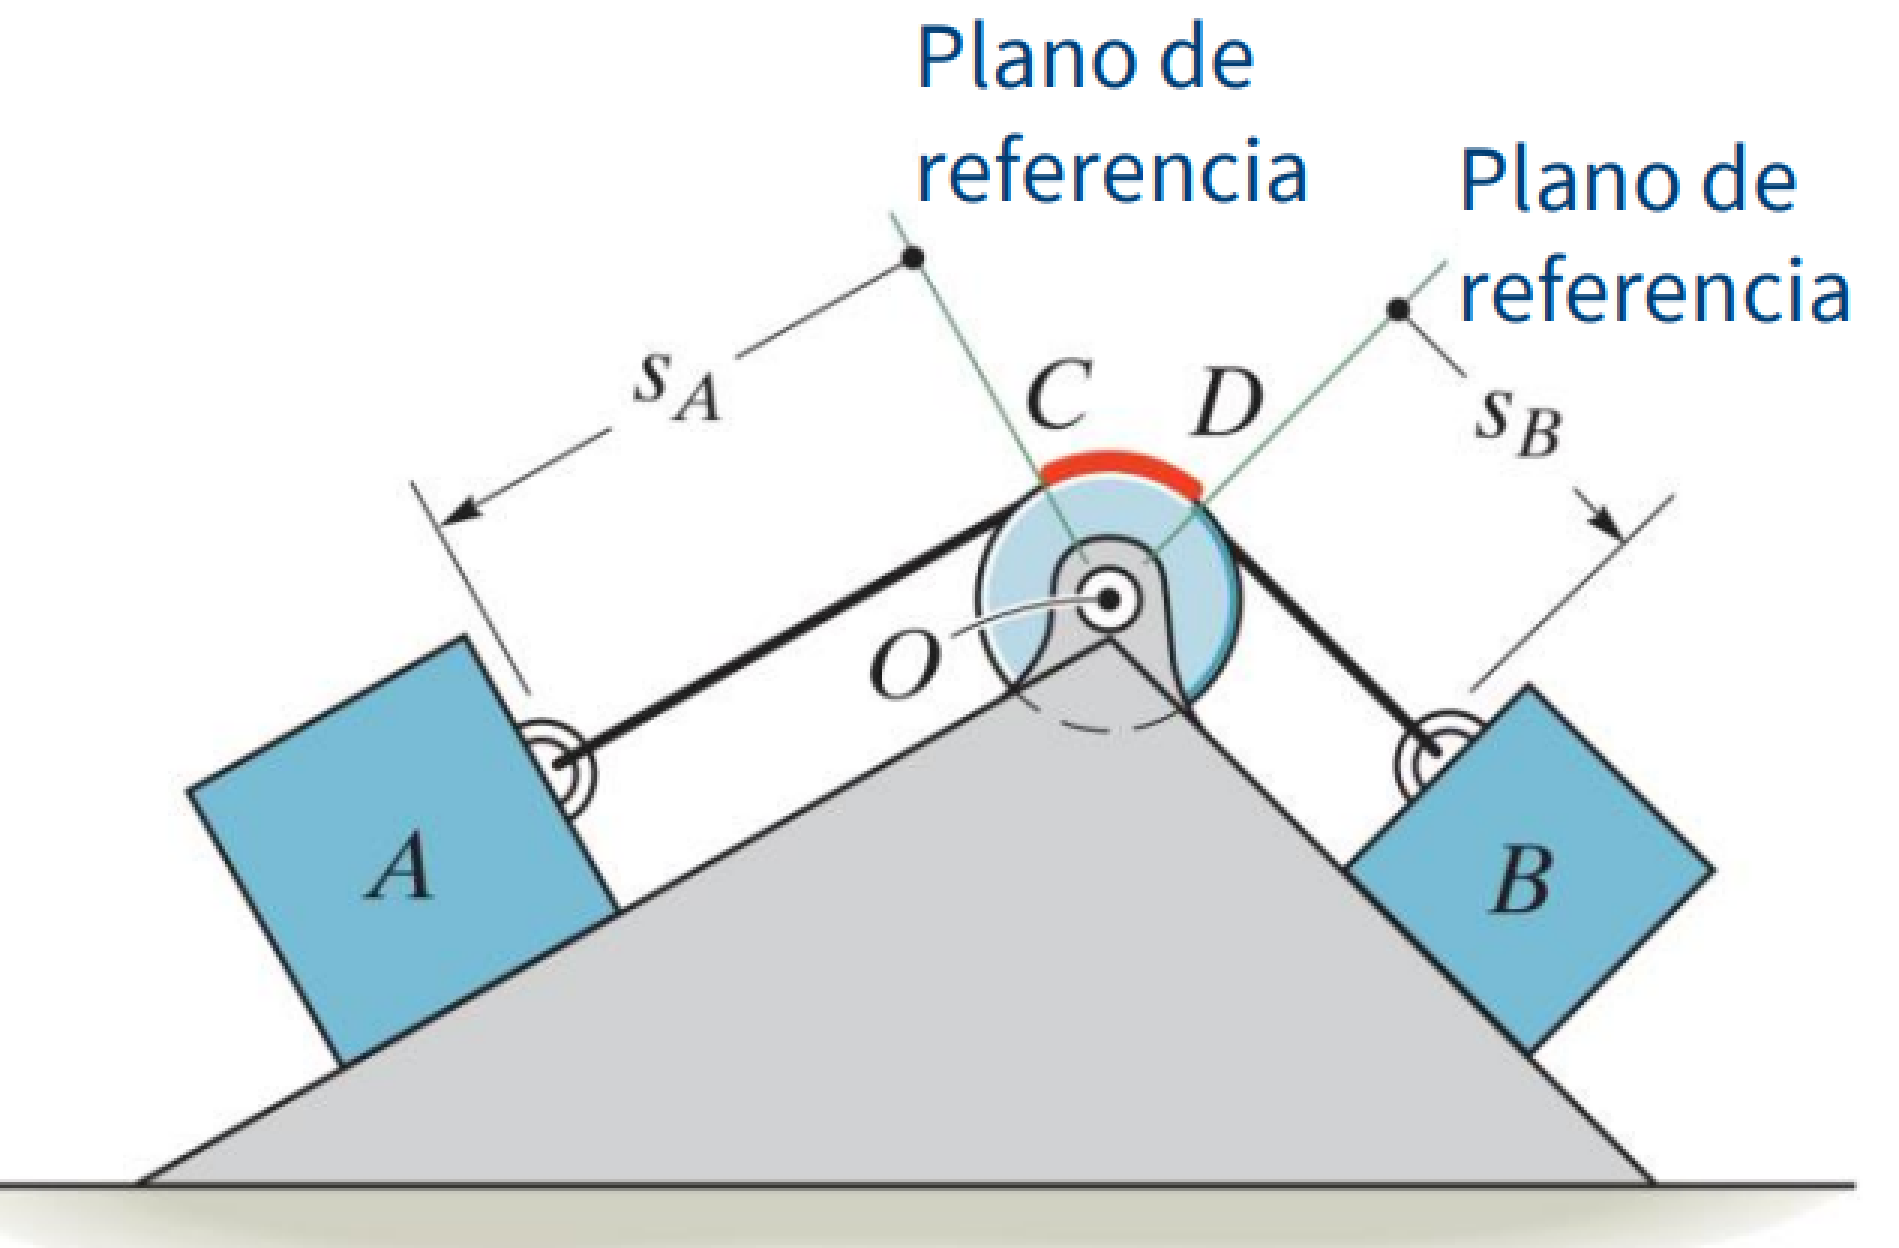
\includegraphics[width=0.5\textwidth]{db24.png}}
  \caption{Movimiento dependientes de partículas}
  \label{db24}
\end{figure}

\begin{equation}
    S_A+l_{CD}+S_B=l_T
\end{equation}

donde $l_T$ es la longitud total de la cuerda, $l_{CD}$ es la longitud de
la cuerda que pasa sobre el arco $CD$.
Si tomamos la derivada con respecto al tiempo de esta
expresión, tenemos

\begin{align*}
    &\frac{dS_A}{dt}+\frac{dS_B}{dt}=0&& v_B=-v_A
\end{align*}

La diferenciación con respecto al tiempo de las velocidades tiene
como resultado la relación entre aceleraciones, $a_B=-a_A$

En la figura (\ref{db25}) se muestra otro ejemplo. Si $l$ representa la longitud
total de la cuerda menos los segmentos (constantes) que enrollan a
las poleas, entonces las coordenadas de posición pueden
relacionarse usando la ecuación

\begin{figure}[h!]
  \centerline{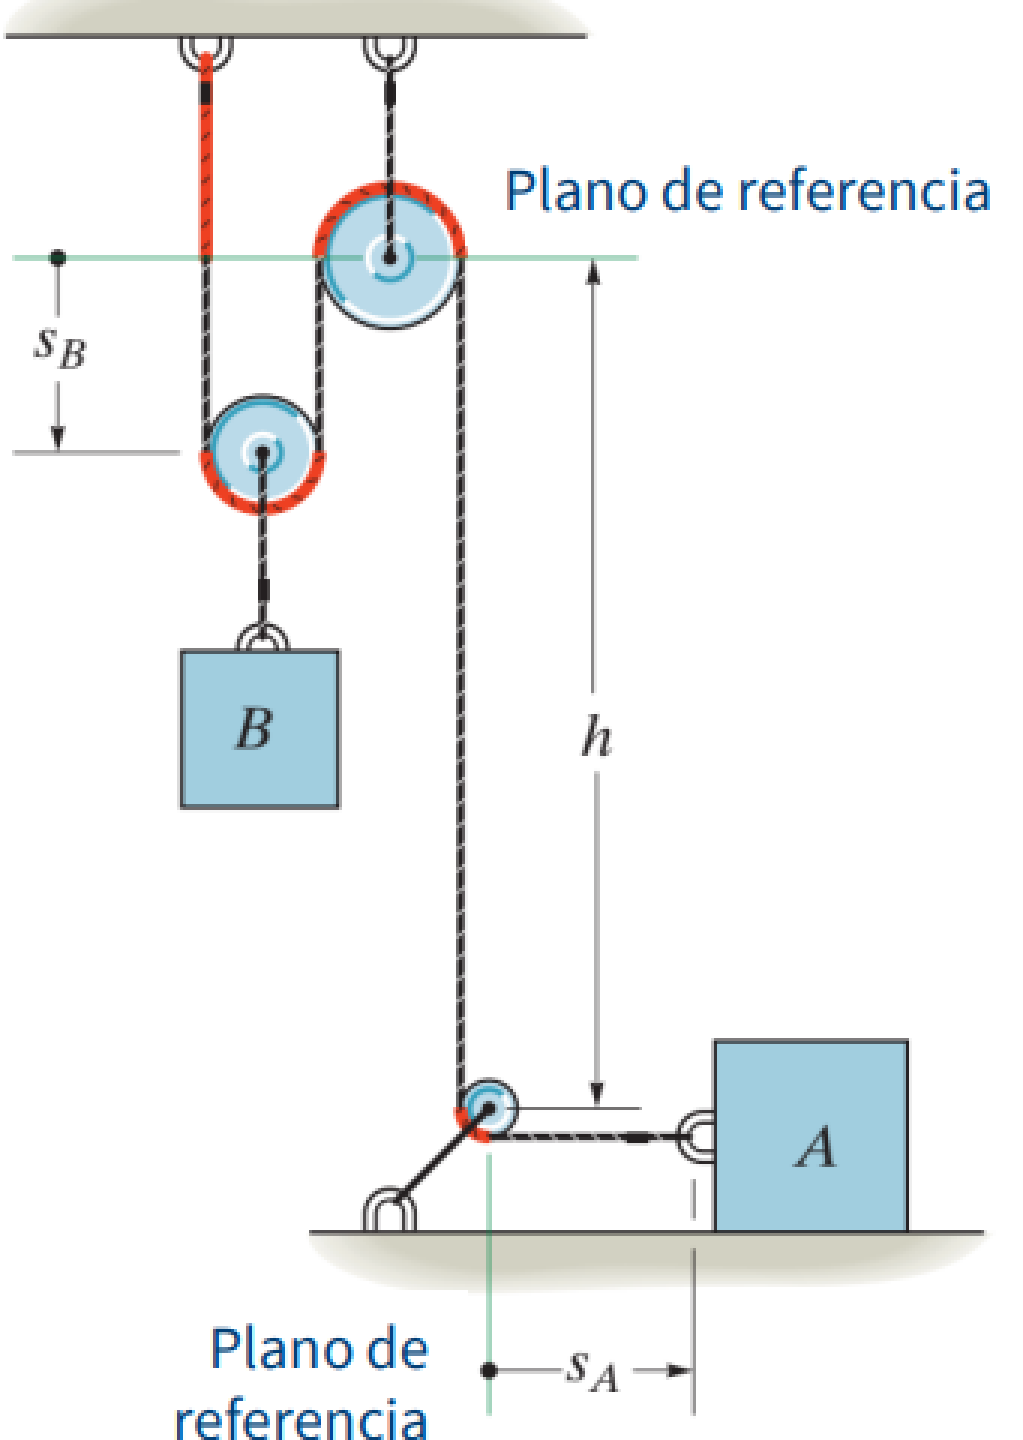
\includegraphics[width=0.5\textwidth]{db25.png}}
  \caption{Ejemplo sobre el movimiento dependientes de partículas}
  \label{db25}
\end{figure}

\begin{equation}
    2S_B+h+S_A=l
\end{equation}

Como $l$ y $h$ permanecen constantes durante el movimiento, las dos
derivadas con respecto al tiempo resultan

\begin{align*}
    &sv_B=-v_A&& 2a_B=-a_A
\end{align*}

Por consiguiente, cuando B se mueve hacia abajo ($+S_B$), A lo hace a
la izquierda ($-S_A$) con el doble del movimiento.

Si se define la posición del bloque B con respecto al centro de la
polea inferior (un punto fijo) (figura \ref{db26}), en este caso,

\begin{figure}[h!]
  \centerline{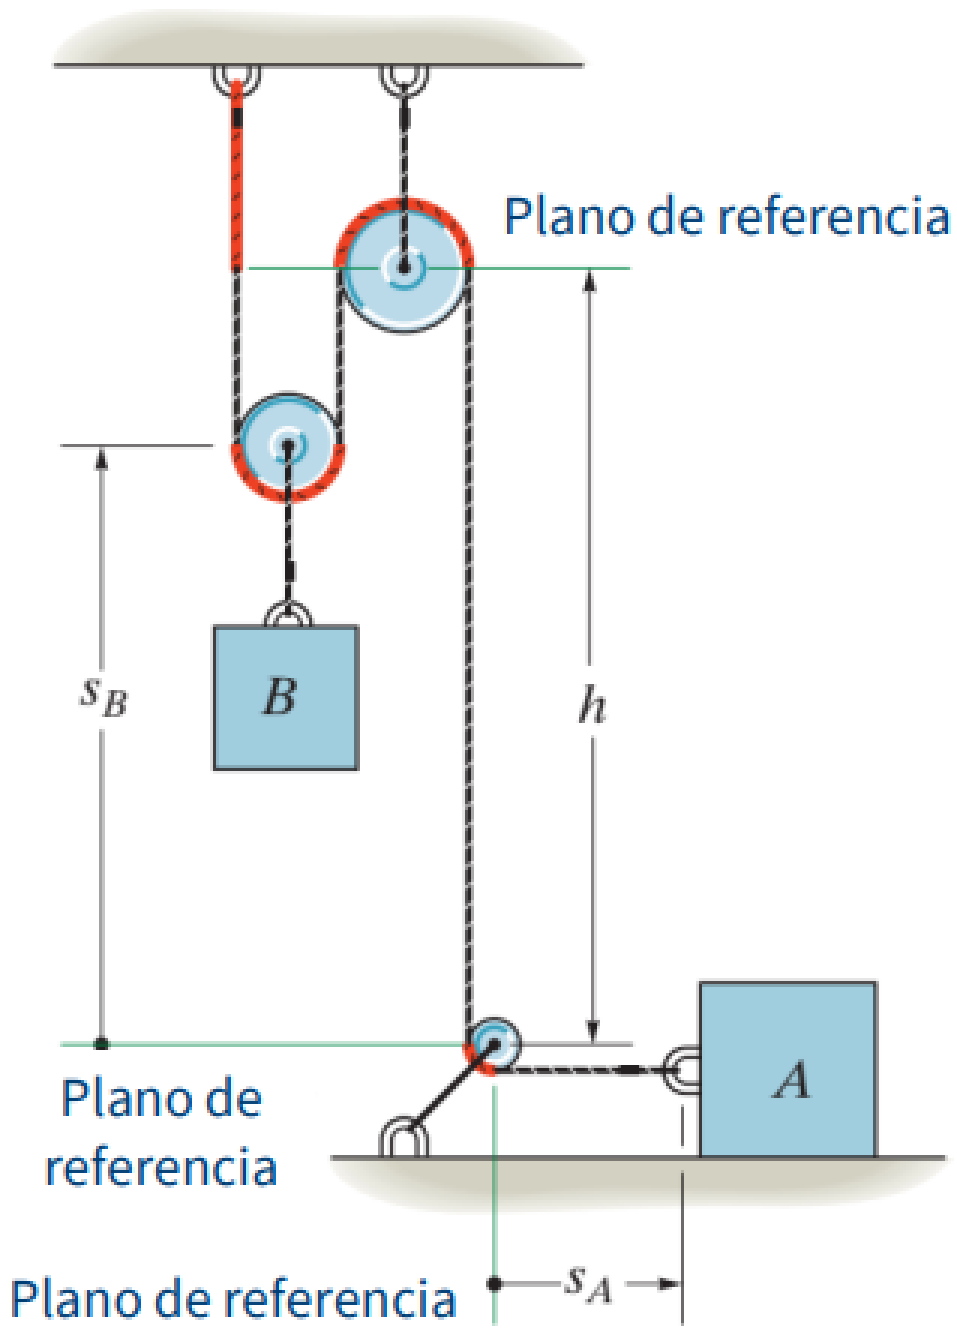
\includegraphics[width=0.5\textwidth]{db26.png}}
  \caption{Siguiente ejemplo}
  \label{db26}
\end{figure}

\begin{equation}
    w(h-S_B)+h+S_A=l
\end{equation}
La diferenciación con respecto al tiempo resulta

\begin{align*}
    2v_B=v_A&&2a_B=a_A
\end{align*}

\begin{example}
    El embalaje $C$ se eleva al mover el rodillo en $A$ hacia abajo
con una rapidez constante de $v_A = 2 m/s$ a lo largo de la guía.
Determine la velocidad y la aceleración del embalaje en el instante $s =1m$. 
Cuando el rodillo está en $B$, el embalaje descansa en el suelo.
Para realizar los cálculos, desprecie el tamaño de la polea. Sugerencia:
Relacione las coordenadas $x_C$ y $x_A$ usando la geometría del problema;
luego, obtenga la primera y segunda derivadas con respecto al tiempo.
\end{example}

\begin{figure}[h!]
  \centerline{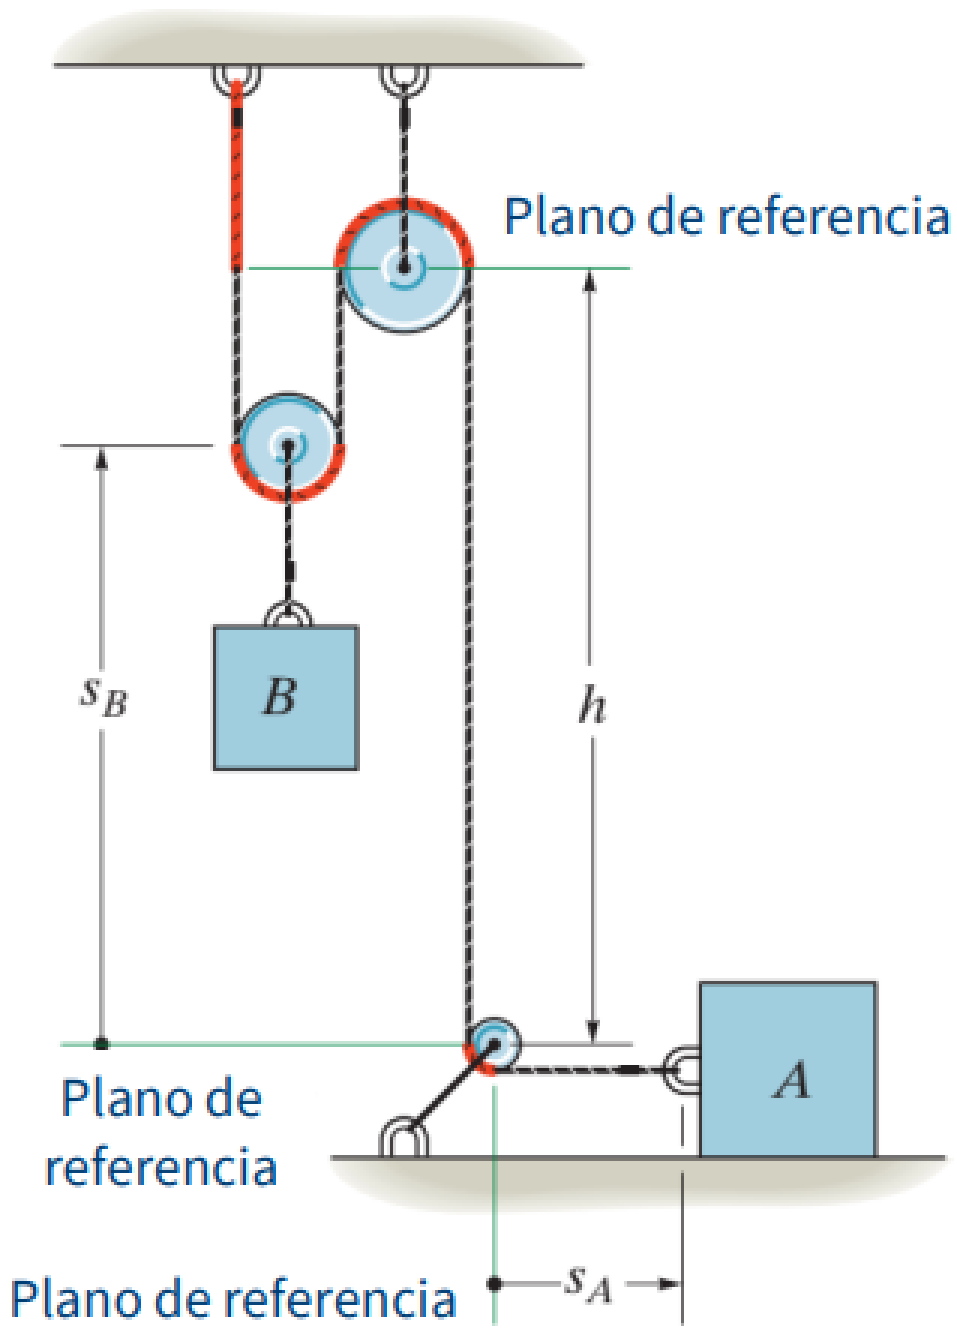
\includegraphics[width=0.5\textwidth]{db27.png}}
  \caption{Esquema del problema}
  \label{db27}
\end{figure}

\textit{ Sol. }

\begin{align*}
    &x_c+\sqrt{x_A^2+4^2}=l\\
    &\dot{x}_c+\frac{1}{2}\left(x_A^2+16\right)^{-\frac{1}{2}}(2x_A)(\dot{x}_A)=0\\
    &\ddot{x}_c-\frac{1}{2}\left(x_A^2+16\right)^{-3/2}\left(2x^2_A\right)^2(\dot{x}^2_A)+\left(x^2_A+16\right)^{-\frac{1}{2}}\left(\dot{x}_A\right)^2\left(x_A^2+16\right)^{-\frac{1}{2}}(x_A)(\ddot{x}_A)=0
\end{align*}

Del problema, $l=8m$ y cuando $s=1m$,
\begin{align*}
    &x_c=4-1=3m\implies x_A=3m\\    &v_A=\dot{x}_A=2m/s\implies a_A=\ddot{x}_A=0m/s^2
\end{align*}

\begin{align*}
    &v_c+\frac{1}{2}\left(3^2+16\right)^{-\frac{1}{2}}(2\cdot 3)(2)=0\\
    &v_c=-1.2m/s=1.2m/s\uparrow \\
    &a_c-\frac{1}{2}\left(3^2+16\right)^{-3/2}\left(2\cdot 3^2\right)(2)^2+\left(3^2+16\right)^{-\frac{1}{2}}(2)^2+\left(3^2+16\right)^{-\frac{1}{2}}(3)(0)=0\\
    &a_c=-0.512m/s^2=0.512m/s^2 \uparrow
\end{align*}

\section{Cinética de una partícula}
\subsection{Segunda ley de Newton del movimiento}
La cinética es una rama de la dinámica que se ocupa de la relación entre el cambio de movimiento de un cuerpo y las fuerzas que lo provocan. La base es la segunda ley de Newton, la cual se puede enunciar de la siguiente manera: 

\emph{Si la fuerza resultante que actúa sobre una partícula no es cero, la partícula tendrá una aceleración proporcional de esta fuerza resultante}

\begin{equation}
    F=m\cdot a
\end{equation}

Donde $F$ es la fuerza, $a$ es la aceleración y $m$ es la masa

La validez de esta ley se basa sólo en evidencia experimental. La ley de Newton de la atracción gravitacional la ley rige la atracción mutua entre dos partículas cualesquiera: 

\begin{equation}
    F=g\cdot \frac{m_1\cdot m_2}{r^2}
\end{equation}

Donde $F$ es la fuerza de atracción entre dos partículas, $G$ la constante de gravitación universal $66.73\left(10^{-12}\right)m^3/kg\cdot s^2$, $m_1,m_2$ masa de cada una de las partículas, y $r$ la distancia entre los centros de las dos partículas.

Peso $W$ de una partícula de masa $m$ sobre la superficie de la tierra, está dada por: 

\begin{equation}
    W=m\cdot g
    \label{eqpeso}
\end{equation}

donde $g$ es la aceleración de la gravedad $g=9.81m/s^2$ ó $g=32.2ft/s^2$.
En el sistema internacional (SI), la masa de un cuerpo se especifica en kg y el peso se calcula con la ecuación
\eqref{eqpeso}, en el sistema FPS (pues, libras, segundos), el peso de un cuerpo se especifica en libras. La masa se 
mide en slugs y se calcula con: $m=2/g(slug)$

\subsubsection{Ecuación de movimiento}
Cuando más de una fuerza actúa en una partícula, la ecuación de movimiento se escribe como: 
\begin{equation}
    \sum F=m\cdot a
\end{equation}
donde $F_R=\sum F$ es la fuerza resultante.
Cuando se aplica la ecuación de movimiento, es importante que la aceleración de la partícula se mida con respecto a un marco de referencia que esté fijo o en traslación 
con velocidad constante, que se conoce como marco de referencia inercial. Cuando se estudian problemas de dinámica que implican movimientos en la superficie terrestre, o cerca de ésta, pueden resolverse con un marco inercial que se supone fijo en la tierra.

Al descomponer cada fuerza $F$ y la aceleración $a$ en componentes rectangulares, se denota como: 

\begin{align*}
    &\sum F=ma&& \sum F_xi+\sum F_yk+\sum F_zk=m\left(a_xi+a_yj+a_zk\right)
\end{align*}
de lo que se deduce que: 
\begin{align*}
    &\sum F_x=ma_x&&\sum F_y=ma_y&&\sum F_z=ma_z
\end{align*}
Como las componentes de la aceleración son iguales a la segunda derivada de la partícula, se tiene:
\begin{align*}
    &\sum F_x=m\ddot{x}&&\sum F_y=m\ddot{y}&&\sum F_z=m\ddot{z}
\end{align*}
Considere el movimiento de un proyectil con peso $W=-Wj$
\begin{align*}
    &m\ddot{x}=0&&m\ddot{y}&&m\ddot{z}=0
\end{align*}
y los componentes de la aceleración del proyectil corresponden a: 
\begin{align*}
    \ddot{x}=0&&\ddot{y}=-\frac{W}{m}=-g&&\ddot{z}=0
\end{align*}
donde $g$ es $9.81 m/s^2$ o $32.2 ft/s^2$.

\subsubsection{Cinética en coordenadas rectangulares}

\begin{example}
    Si el embalaje de 50 kg parte del reposo y alcanza una velocidad de $v=4 m/s$ al recorrer una distancia de 5 m hacia la derecha, determine la magnitud de la fuerza $P$ que actúa sobre el embalaje. El coeficiente de fricción cinética entre el embalaje y el suelo es $\mu k = 0.3$.
\end{example}

\begin{figure}[h!]
\centering
  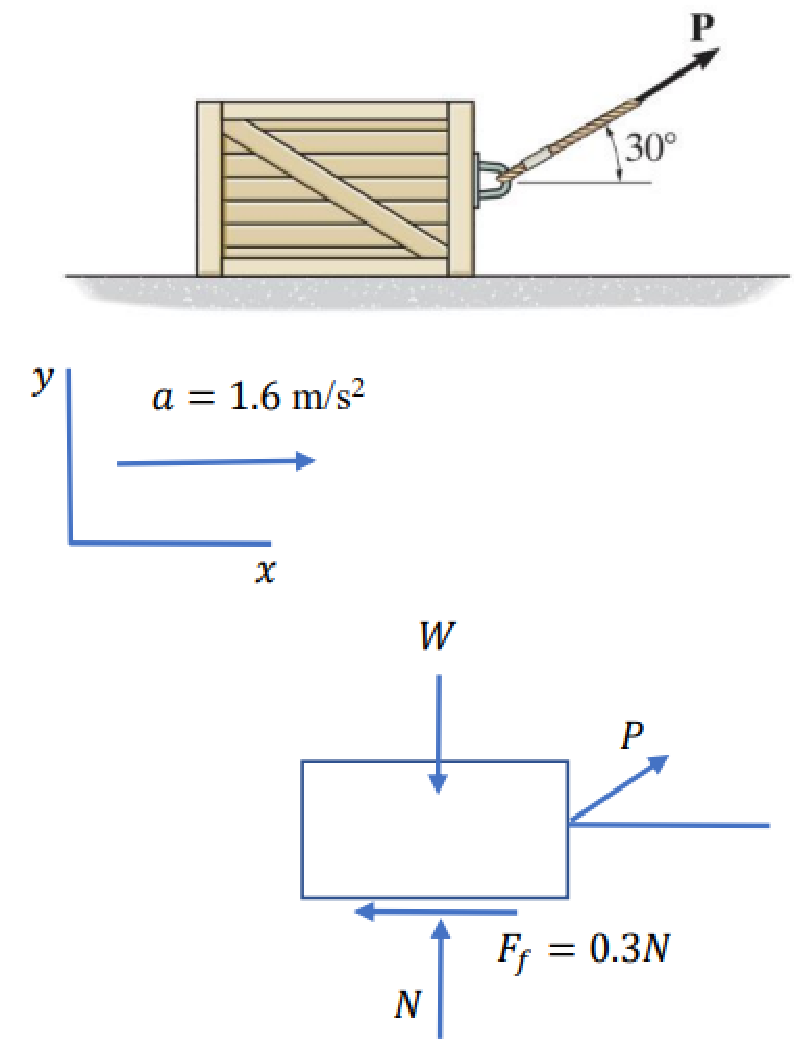
\includegraphics[width=0.5\textwidth]{db28.pdf}
  \caption{Cinética en coordenadas rectangulares}
  \label{db28}
\end{figure}

\textit{ Sol. }

Cinemática
\begin{align*}
    &v^2=v^2_0+2a_c(s-s_0)\\
    &4^2=0^2+2a(5-0)\\
    &a=\frac{16}{10}=1.6m/s^2
\end{align*}

Diagrama de cuerpo libre. Fuerza de fricción cinética
\begin{equation*}
    F_f=\mu_k N=0.3N
\end{equation*}
Ecuaciones de movimiento
\begin{align*}
    &\sum F_y=ma_y\\
    &N+P\sin{(30^{\circ})}-(50)(9.81)=50(0)\\
    &N=490.5-P\sin{(30^{\circ})}\\
    &\sum F_x=ma_x\\
    &P\cos{(30^{\circ})}-0.3(490.5-P\sin{(30^{\circ})})=50(1.6)\\
    &P\cos{(30^{\circ})}-0.3 490.5 + 0.3P \sin{(30^{\circ})} = 50(1.6)\\
    &P \left(\cos 30^{\circ} + 0.3\sin{30^{\circ}}\right) - 0.3(490.5)=50(1.6)\\
    &P\left(\cos 30^{\circ} + 0.3 \sin 30^{\circ}\right) = 50 (1.6) + 0.3 (490.5)\\
    &P=\frac{50(1.6)+0.3(490.5)}{\cos{(30^{\circ})+0.3\sin{(30^{\circ}})}}=223.57N=224N
\end{align*}

\subsubsection{Cinética en componentes normal y tangencial}

Al descomponer las fuerzas y la aceleración de la partícula en componentes a lo largo de la tangente a la trayectoria (en la dirección del movimiento) y la normal (hacia el interior de la trayectoria) y sustituir en la ecuación de movimiento

\begin{align*}
    \sum F=ma&&\sum F_tu_t+\sum F_nu_n=ma_t+ma_n
\end{align*}
se obtienen las dos ecuaciones escalares
\begin{align*}
    &\sum F_t=ma_t&&\sum f_n=ma_n
\end{align*}
Al sustituir $a_t=\frac{dv}{dt}$ y $a_n=\frac{v^2}{p}$ en estas últimas ecuaciones se obtiene
\begin{align*}
    &\sum F_t=m\frac{dv}{dt}&&\sum f_n=m\frac{v^2}{p}
\end{align*}
Las ecuaciones que se obtienen pueden resolverse para dos incógnitas.

\begin{example}
    Se requiere mover cajas de cartón con una masa de 5 kg a lo largo de la línea de ensamble a una rapidez constante de 8 m/s. Determine el radio de curvatura más pequeño, P, para el transportador, de modo que las cajas de cartón no se deslicen. Los coeficientes de fricción estática y cinética entre una caja de cartón y el transportador son $\mu_s= 0.7$ y$ \mu_k= 0.5$ , respectivamente.
\end{example}
\begin{figure}[h!]
\centering
  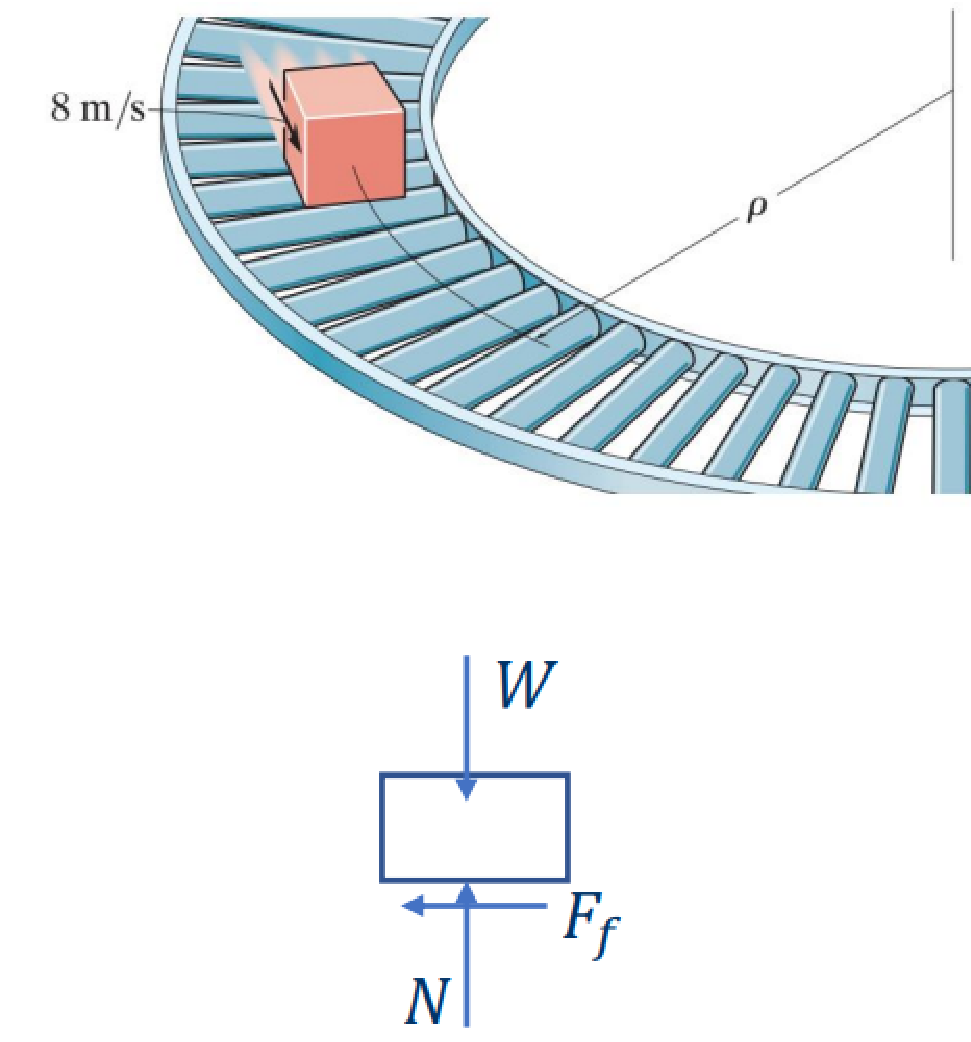
\includegraphics[width=0.5\textwidth]{db29.pdf}
  \caption{cajas de cartón}
  \label{db29}
\end{figure}

\textit{ Sol. }
\begin{align*}
    &+\uparrow \sum F_b=ma_b&&N_w=0\\
    &N=w&&F_f=\mu_sN=0.7W\\
    &+\leftarrow \sum F_n=ma_n&&F_f=m\left(\frac{8^2}{p}\right)\\
    &0.7(5\times 9.81)=5\left(\frac{8^2}{P}\right)&&P=9.31
\end{align*}

\begin{example}
    La bola B del péndulo tiene un peso de 30 kg y se suelta desde el reposo en la posición mostrada, $\theta= 0^{\circ}$. Determine la tensión en la cuerda BC justo después de que se liberó la bola, $\theta=0^{\circ}$ y también en el instante en que la bola alcanza $\theta= 45^{\circ}$. Considere que $r= 4 m$
\end{example}

\textit{ Sol. }

Ecuaciones de movimiento
\begin{align*}
    &\theta = 0^{\circ}&&v = 0\\
    &\sum F_n = ma_n&& T = m\left(\frac{v^2}{r}\right) = 30\left(\frac{0^2}{4}\right) = 0N\\
    &\theta = 5^{\circ}&&\sum F - t = ma_t\\
    &W\cos{(\theta)}&&30a_t\\
    &a_t = 9.81\cos{(\theta)}\frac{m}{s^2}&&\sum F_n = ma_n\\
    &T - W\sin{(45^{\circ})} = m\left(\frac{v^2}{r}\right)&&T -(30\cdot 9.81)\sin{(45^{\circ})} = m\left(\frac{v^2}{4}\right)
\end{align*}
Cinemática: La velocidad de la bola cuando $\theta= 45^{\circ}$ se puede determinar usando $v\,dv=at\,ds$.
También $ds=r\,d\theta$, entonces $v\,dv= atr\,d\theta=4at\, d\theta$. Integrando:
\begin{align*}
    &\int_0^v v\,dv = 4(9.81)\int_0^{45^{\circ}}\cos{(\theta)}\,d\theta = 4(9.81)\left[\sin{(\theta)}\right]_{0^{\circ}}^{45^{\circ}}\\
    &v^2 = 2(39.24)\left(\frac{\sqrt{2}}{2}\right) = 55.49\, v = \frac{7.45m}{s}\\
    &T = 30\left(\frac{7.45^2}{4}\right) +(30\cdot 9.8)\sin{(45^{\circ})} = 624.34,\, T = 624.34N
\end{align*}

\subsubsection{Cinética en coordenadas cilíndricas}

Cuando todas las fuerzas que actúan en una partícula se descomponen en sus componentes cilíndricas, la ecuación de movimiento se expresa como
\begin{align*}
    &\sum F =ma\\
    &\sum F_ru_r + \sum F_{\theta}u_{\theta} \sum F_zu_z = ma_r u_r + ma_{\theta}u_{\theta} + ma_zu_z\\
    &\sum F_r = a_r\, \sum F_r m\left(\ddot{r}- r \dot{\theta}^2\right)\\
    &\sum F_{\theta} = ma_{\theta}\, \sum F_{\theta}= m\left(r\ddot{\theta} 2dot{r}\dot{\theta}\right)\\
    &\sum F_z = ma_z\, \sum F_z= m\ddot{z}
\end{align*}
Las direcciones de la fuerza normal $N$ y la fuerza de fricción $F$ pueden especificarse con respecto a la coordenada radial con el ángulo $\Psi$, el cual se define entre la línea radial extendida y la tangente a la curva.
\begin{equation}
    \tan{(\Psi)} = \frac{r}{\frac{dr}{d\theta}}
\end{equation}

\begin{figure}[h!]
\centering
  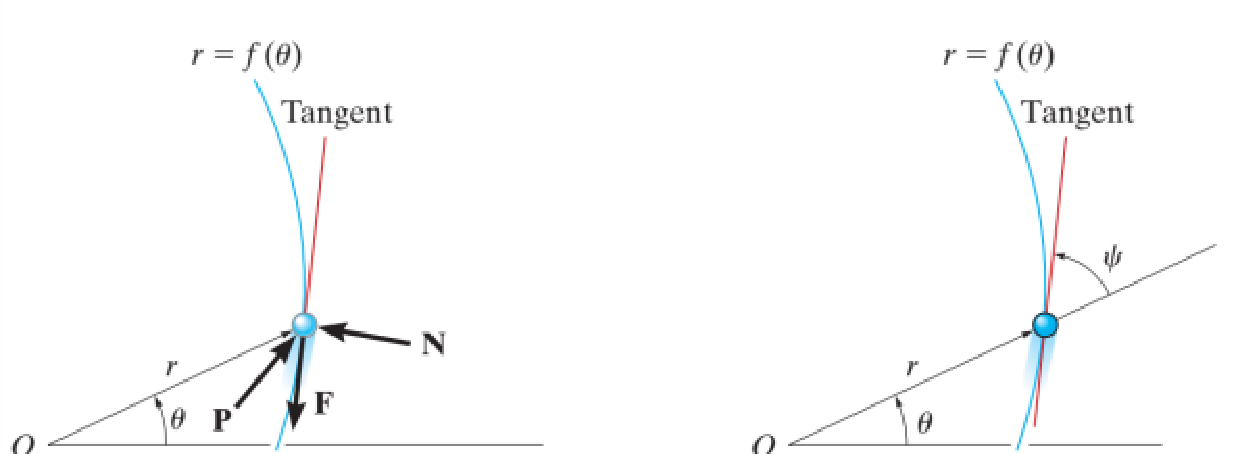
\includegraphics[width=0.5\textwidth]{db30.pdf}
  \caption{Cinética en coordenadas cilíndricas}
  \label{db30}
\end{figure}

\begin{example}
    Un bloque $B$ de masa $m$ puede deslizarse libremente sobre un brazo $OA$ sin fricción, que gira en el plano horizontal a razón constante $\dot{\theta}_0$ Si se sabe que $B$ se suelta a una distancia $r_0$ de O, exprese como función de $r$,
\begin{itemize}
    \item la componente $vr$ de la velocidad de B a lo largo de OA
    \item la magnitud de la fuerza horizontal $F$ ejercida sobre B por el brazo OA.
\end{itemize}
\end{example}

\textit{ Sol. }

\begin{align*}
    &\sum F_r = ma_r\, 0 = m\left(\ddot{r} - r\dot{\theta}^2\right)\\
    &\sum F_r = ma_{\theta}\, F= m\left(r\ddot{\theta} + 2\dot{r}\dot{\theta}\right)
\end{align*}

Componente $v_r$ de la velocidad. Como $vr=\dot{r}$, se tiene
\begin{equation*}
    \ddot{r} =\dot{v}_r =\frac{dv_r}{dt} =\frac{dv\,r\dot dr}{dr\cdot dt} = v_r\cdot \frac{dv_r}{dr}
\end{equation*}
De la ecuación $0=\ddot{r}-r\dot{\theta}^2$, de donde $\ddot{r}=r\dot{\theta}^2$
\begin{align*}
    &v_r\cdot \frac{dv_r}{dr} = r\dot{\theta}^2\\
    &v_rdv_r =\dot{\theta}_0^2r\,dr\\
    &\int_0^{v_r}v_r\,dv_r =\dot{\theta}_0^2\int_{r_0}^rr\,dr\\
    &\frac{v_r^2}{2} =\frac{\dot{\theta}_0^2}{2}\left(r^2 - r^2_0\right)2
    v_r = \sqrt{\dot{\theta}_0^2\left(r^2 - r_0^2\right)} =\dot{\theta}_0\sqrt{r^2 - r_0^2}
\end{align*}
Fuerza horizontal. Sustituyendo en la ecuación $\dot{\theta}=\dot{\theta}_0$, $\ddot{\theta}=0,\dot{r}=v_r$
\begin{align*}
    &F = m\left(r(0) + 2v_r\dot{\theta}_0\right) = 2m\dot{\theta}_0 v_r =2m\dot{\theta}_0\left(\dot{\theta}_0\sqrt{r^2 - r_0^2}\right)\\
    &F = 2m\dot{\theta}_0^2\sqrt{r^2 - r_0^2}
\end{align*}

\begin{example}
    Si la posición del anillo $C$ de 3 kg sobre la barra lisa $AB$ se mantiene en $r= 720 mm$, determine la velocidad angular constante $\dot{\theta}$ a la cual gira el mecanismo en torno al eje vertical. La longitud no alargada del resorte es de 400 mm. Ignore la masa de la barra y el tamaño del anillo.
\end{example}
\begin{figure}[h!]
\centering
  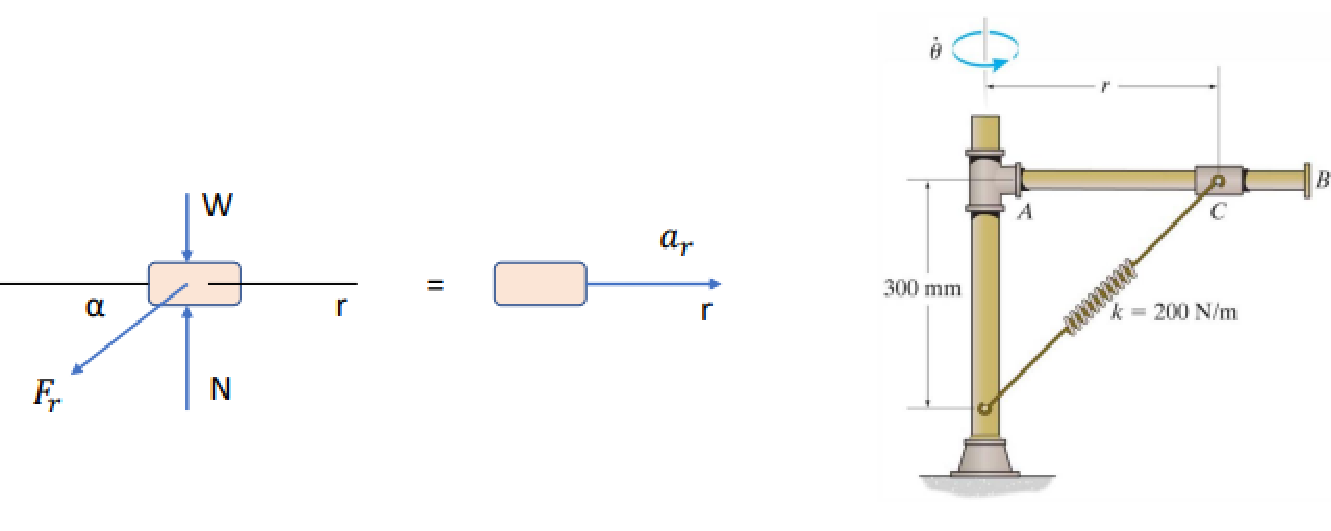
\includegraphics[width=0.5\textwidth]{db31.pdf}
  \caption{Esquema del problema}
  \label{db31}
\end{figure}
\textit{ Sol. }

Fuerza del resorte:
\begin{equation*}
    F_r = kx = 200\left(\sqrt{0.3^2 + 0.72^2} - 0.4\right) = 76N
\end{equation*}
Ecuaciones de movimiento:

\begin{align*}
    &+\rightarrow \sum F_r = ma_r\, -(76)\cos{(\alpha)} = 3a_r\\
    &-(76)\left(\frac{0.72}{\sqrt{0.3^2 + 0.72^2}}\right) = 3a_r\\
    &- 76\left(\frac{12}{13}\right) = 3a_r\\
    &-76\left( \frac{12}{13} \right)\implies a_r =-\frac{76}{3} \left(\frac{12}{13}\right) =- 23.38
\end{align*}

Cinemática: Como $r$ es constante:
\begin{align*}
    &\dot{r}=\ddot{r}=0\\ 
    &a_r =\ddot{r} - r\dot{\theta}^2 = 0 -(0.72)(\ddot{\theta}^2)\\
    &- 23.38 =-(0.72)(\dot{\theta}^2)\\
    &\dot{\theta} = \sqrt{\frac{23.38}{0.72}} = 5.6990 = 5.70\frac{rad}{s}\\
    &\dot{\theta} = 5.70 \frac{rad}{s}
\end{align*}

\begin{example}
    Si el coeficiente de fricción estática entre el bloque de masa $m$ y la tornamesa es $\mu s$, determine la velocidad angular constante máxima de la plataforma sin que el bloque se deslice.
\end{example}

\begin{figure}[h!]
\centering
  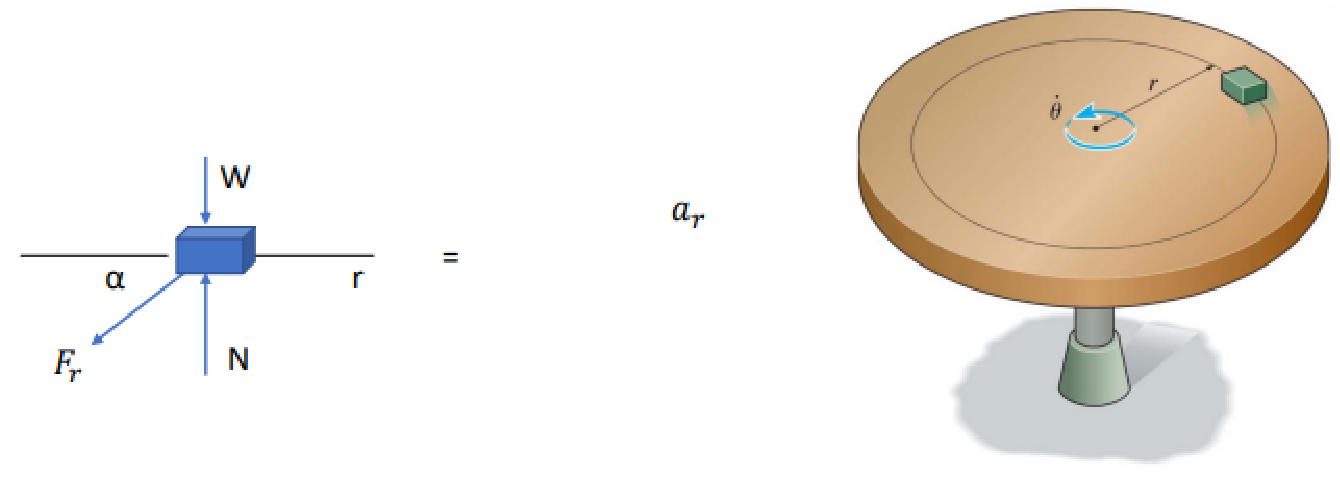
\includegraphics[width=0.5\textwidth]{db32.pdf}
  \caption{Cinética en coordenadas cilíndricas}
  \label{db32}
\end{figure}
Ecuaciones de movimiento
\begin{align*}
    &\sum F_r = ma_r\, - F_r = ma_r\\
    &\sum F_{\theta} = ma_{\theta}\, F_{\theta} = ma_{\theta}\\
    &\sum F_z = ma_z\, N - mg = m(0)\mid N = mg 
\end{align*}
Cinemática: Como $r$ y $\dot{\theta}$ son constantes: $\dot{r}=\ddot{r}=0$, $\ddot{\theta}=0$
\begin{align*}
    &a_r =\ddot{r} - \dot{\theta}^2 = 0 - r\dot{\theta}^2\\
    &a_{\theta} = r\ddot{\theta} + 3\dot{r}\dot{\theta} = 0
\end{align*}
Sustituyendo $a_r$ y $a_{\theta}$ en las ecuaciones de movimiento:
\begin{align*}
    &- F_r = m( - r\dot{\theta}^2)\, F_r =mr\dot{\theta}^2\\
    &F_{\theta} = m(0)\mid F_{\theta} = 0
\end{align*}
Magnitud de la fuerza:
\begin{equation*}
    F =\sqrt{F_r^2 + F_{\theta}^2} = \sqrt{\left(mr\dot{\theta}^{2}\right)^2} + 0^2 = mr\dot{\theta}^2
\end{equation*}
Se requiere que el bloque no se deslice,
\begin{equation*}
    F =\mu_s N =\mu_s mg
\end{equation*}
Entonces: 
\begin{align*}
    &\mu_s mg = mr\dot{\theta}^2\\
    &\frac{\mu_s g}{r} =\dot{\theta}^2\\
    &\theta = \sqrt{\frac{\mu_s g}{r}}
\end{align*}

El método del trabajo y la energía relaciona directamente la fuerza, la masa, la velocidad y el desplazamiento. El método de trabajo y energía es útil para calcular el cambio de rapidez durante un desplazamiento de la partícula. Una fuerza $F$ realizará trabajo en una partícula sólo cuando ésta sufra un desplazamiento en la dirección de la fuerza. La fuerza $F$ hace que la partícula se mueva a lo largo de la trayectoria $s$ de la posición $r$ a la una posición $r^{\prime}$ el desplazamiento es $dr=r^{\prime}-r$. La magnitud de $dr$ es $ds$. El trabajo realizado por $F$ es una cantidad escalar, definida por
\begin{align*}
    &du = Fds\cos{\theta}&&du = F\cdot dr
\end{align*}
Si la componente de la fuerza y el desplazamiento tienen el mismo sentido, el trabajo es positivo. Si éstos vectores tienen sentido opuesto,el trabajo es negativo. Si la fuerza es perpendicular al desplazamiento, $du=0$

\begin{definition}[Trabajo de una fuerza variable.]
    El trabajo hecho por una fuerza $F$ cuando la partícula se mueve
de la posición $r_1$ a $r_2$ se determina mediante integración.
\begin{equation}
    U_{1-2} \int_{r_1}^{r_2}F\cdot dr = \int_{S_1}^{S_2} F\cos{(\theta)}\, ds
\end{equation}
\end{definition}
El área bajo la gráfica de $F\cos{\theta}$ vs $s$ limitada por $s_1$ y $s_2$ representa el trabajo total.
\begin{figure}[h!]
\centering
  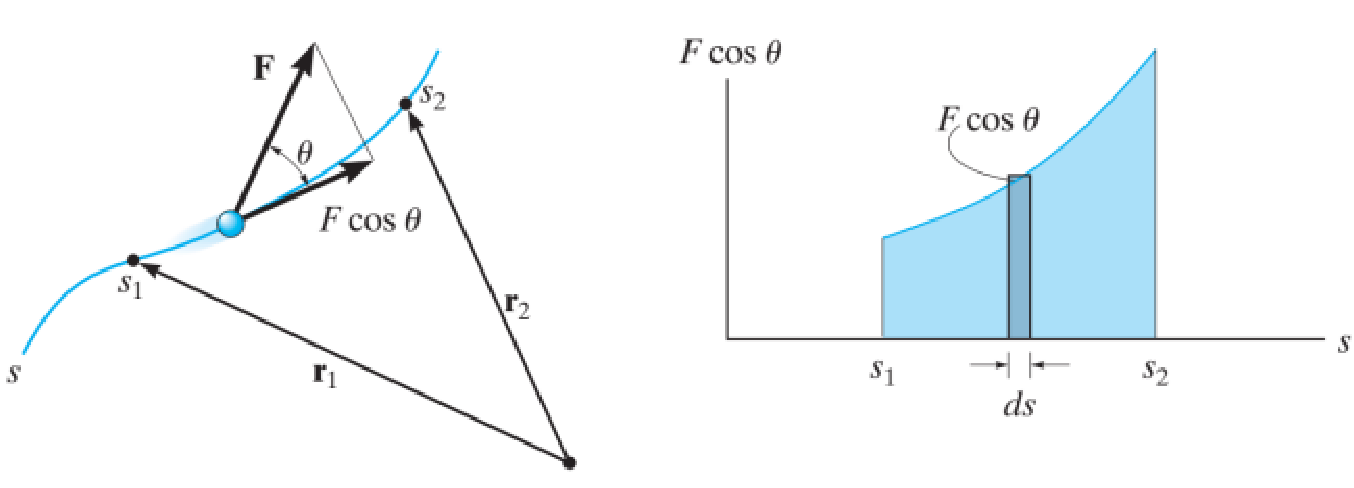
\includegraphics[width=0.5\textwidth]{db33.pdf}
  \caption{Trabajo de una fuerza variable. }
  \label{db33}
\end{figure}
Trabajo de una fuerza constante que se mueve a lo largo de una línea recta. El trabajo realizado por una fuerza $F_c$ constante cuando la partícula se desplaza de $s_1$ a $s_2$ se determina mediante integración.
\begin{align*}
    &U_{1-2} = F_c\cos{\theta}\int_{s_1}^{s_2}\,ds\\
    &U_{1-2} F_c\cos{\theta}\left(s_2 - s_1\right)
\end{align*}
Donde $F_c\cos{\theta}$ es la componente de $F_c$ en la dirección del desplazamiento.
Aquí el trabajo de $F_c$ representa el área del rectángulo.

\begin{figure}[h!]
\centering
  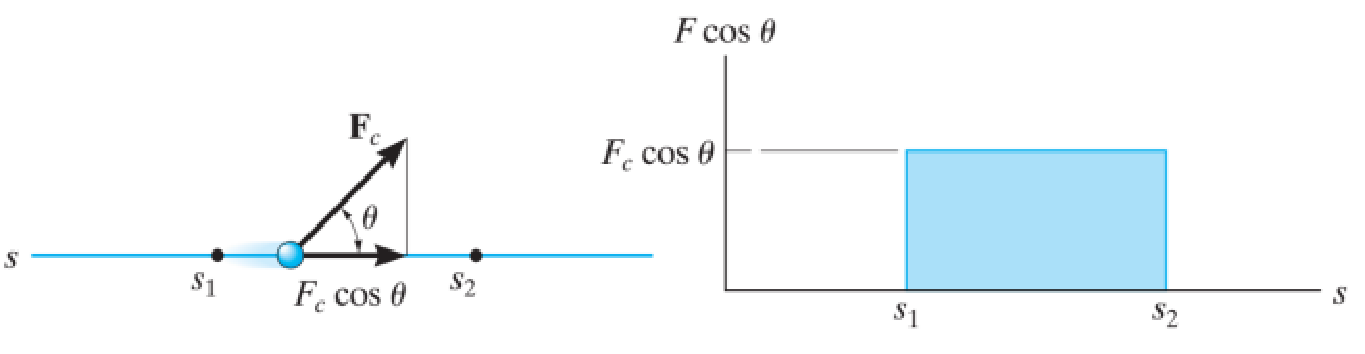
\includegraphics[width=0.5\textwidth]{db34.pdf}
  \caption{Trabajo de una fuerza constante que se mueve a lo largo de una línea recta.}
  \label{db34}
\end{figure}

Trabajo de un peso. Considere una partícula de peso $W=-Wj$, que se mueve a lo largo de la trayectoria $s$ mostrada de la posición $s_1$ a la posición $s_2$. En un punto intermedio, $dr=dxi+dyi+dzk$. Entonces

\begin{align*}
    &U_{1 -2} = \int F\,dr = \int_{r_1}^{r_2}( Wj)(dxi dyj dzk)\\
    &U_{1 -2} = \int_{y_1}^{y_2} - W\,dy - W(y_2 - y_{1})\\
    &U_{1- 2 } =- W\Delta y
\end{align*}
\begin{figure}[h!]
    \centering
      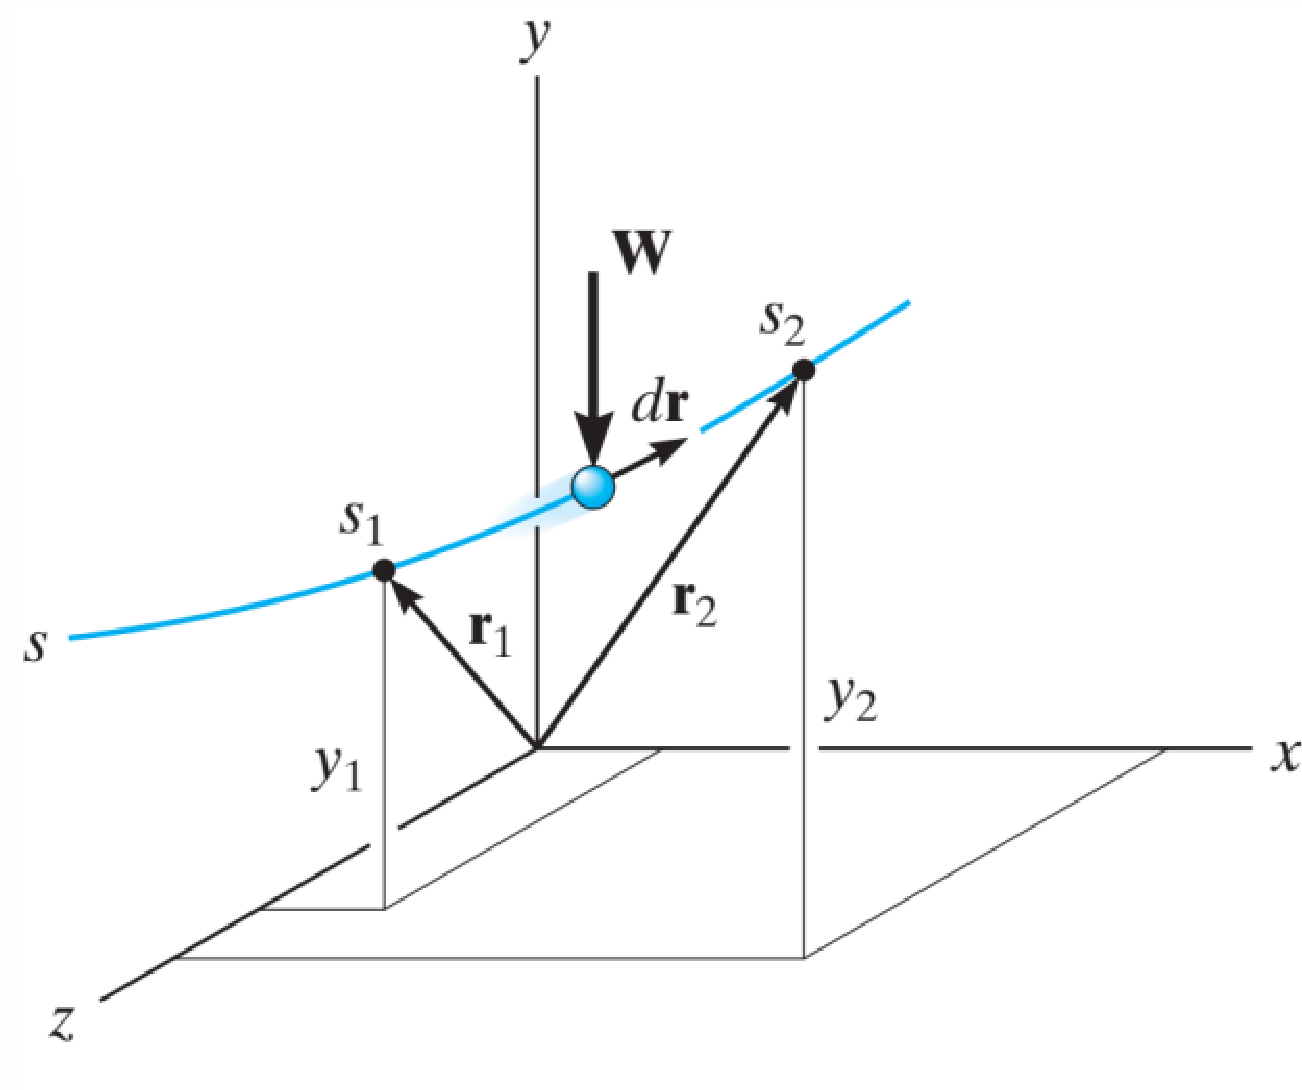
\includegraphics[width=0.5\textwidth]{db35.pdf}
      \caption{Trabajo de un peso}
      \label{db35}
\end{figure}
Entonces, el trabajo es independiente de la trayectoria.

Trabajo de un resorte. Considere un resorte lineal de rigidez $k$ donde la fuerza requerida para comprimir o estirar el resorte es proporcional a la deformación $ds$. El trabajo realizado por la fuerza que actúa en la partícula adjunta es $du=-F_s\,ds=-ks\,ds$. El trabajo es negativo porque $F_s$ actúa en sentido opuesto a $ds$. Si la partícula se desplaza de $s_1$ a $s_2$, el trabajo de $F_s$ es
\begin{equation*}
    U_{1 -2}=\int_{s_1}^{s_2}F_s\,ds =\int_{s_1}^{s_2}-ks\,ds = -\left(\frac{1}{2}ks_2^2 \frac{1}{2}ks_1^2\right)
\end{equation*}
donde $F_c\cos{(\theta)}$ es la componente de $F_c$ en la dirección del desplazamiento.
El trabajo de $F_s$
representa el área trapezoidal bajo la línea $F_s=ks$.
\begin{figure}[h!]
    \centering
      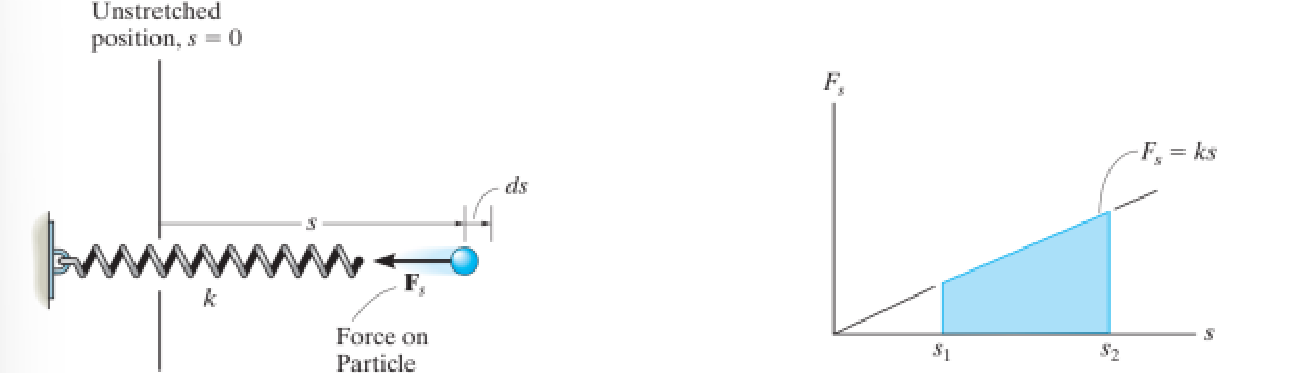
\includegraphics[width=0.5\textwidth]{db36.pdf}
      \caption{Trabajo de un resorte}
      \label{db36}
\end{figure}

\subsubsection{Principio de trabajo y energía.}

Considere una partícula de masa $m$ que se somete a una fuerza $F_R=\sum F$ y que se mueve a lo largo de una trayectoria curvilínea. La ecuación de movimiento de la partícula en la dirección tangencial es $\sum F_t=ma_t$. Si aplicamos la ecuación cinemática $at=\frac{v\,dv}{ds}$ e integramos ambos lados, tenemos
\begin{equation*}
    \sum \int_{s_1}^{s_2}F_t\, ds =\sum U_{1 - 2}= \int_{v_1}^{v_2}mv\,dv
\end{equation*}
Esta ecuación representa el principio de trabajo y energía.

El término del lado izquierdo es la suma del trabajo realizado por todas las fuerzas que actúan en la partícula cuándo ésta se mueve del punto 1 al punto 2. Los dos términos del lado derecho, cuya forma es $T=\frac{1}{2}mv^2$, definen la energía cinética final e inicial, respectivamente. Unidades del trabajo: ($J$) o $libra\cdot pie$. La energía cinética siempre es positiva. Formal alternativa
\begin{equation}
    T_1 +\sum U_{1 - 2}=T_2
\end{equation}
que establece que la energía cinética inicial de la partícula, más el trabajo realizado por todas las fuerzas que actúan en ella cuando se mueve de su posición inicial a su posición final, es igual a la energía cinética final de la partícula. Este principio resulta conveniente cuando se resuelven problemas cinéticos que implican fuerza, velocidad y desplazamiento. 

\begin{example}
    El embalaje de 20 kg se somete a una fuerza que tiene una dirección constante y una magnitud $F = 100 N$. Cuando $s= 15 m$, el embalaje se mueve hacia la derecha con una rapidez de 8 m/s. Determine su rapidez cuando $s = 25 m$. El coeficiente de fricción cinética entre el embalaje y el suelo es $\mu k = 0.25$.
\end{example}
\begin{figure}[h!]
\centering
  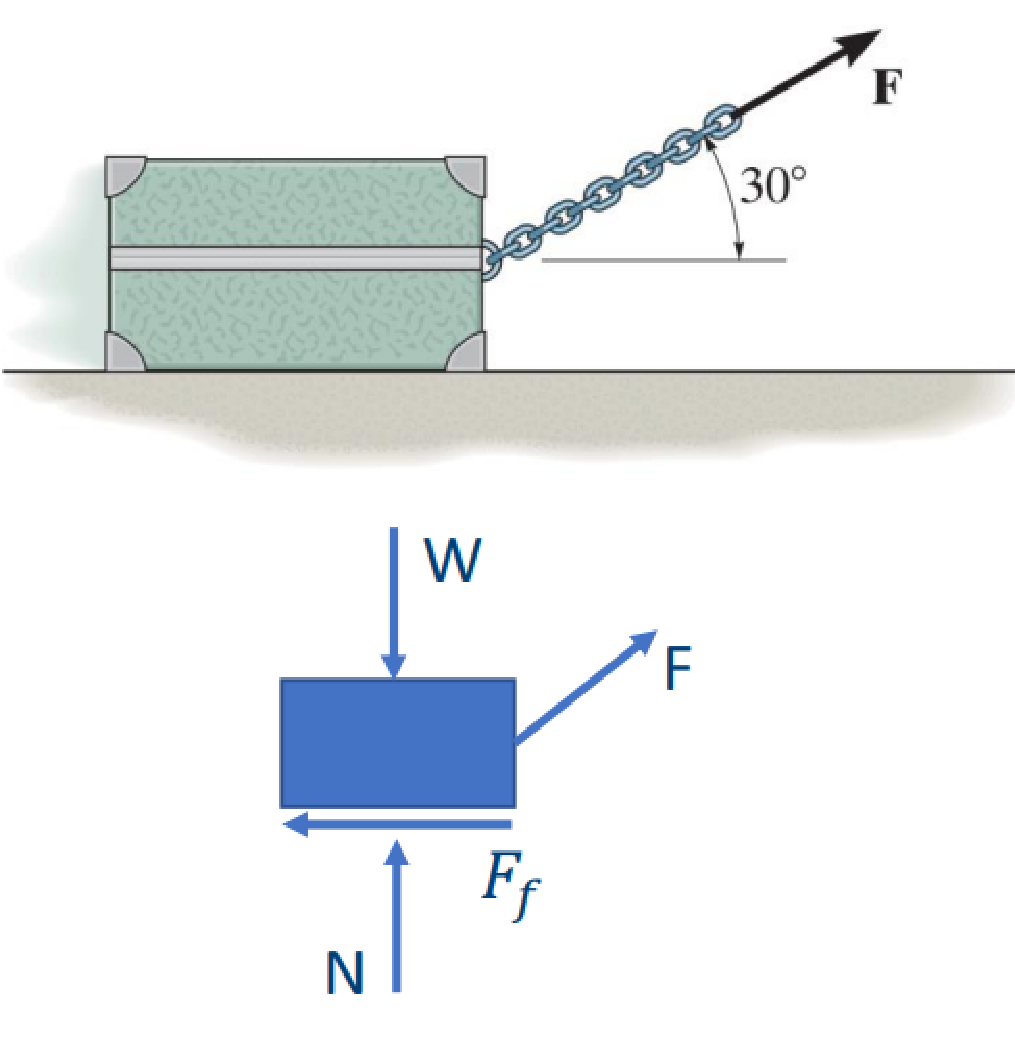
\includegraphics[width=0.5\textwidth]{db37.pdf}
  \caption{Esquema del problema del embalaje}
  \label{db37}
\end{figure}
\textit{ Sol. }
Ecuación de movimiento. Fuerza de fricción desarrollada entre el embalaje y el suelo es $F_f= \mu_k N= 0.25N$.

\begin{align*}
    &+\uparrow \sum F_y = ma_y&& N 100\sin{(30^{\circ})} - 20(9.81) = 20(0)\\
    &N =- 100\sin{(30^{\circ})} +20(9.81) = 146.2N
\end{align*}
Principio de Trabajo y Energía. La componente horizontal de la fuerza $F$ que actúa en la dirección del desplazamiento hace realiza trabajo positivo, mientras que la fuerza de fricción $F_f$ hace trabajo negativo. La fuerza de reacción $N$, la componente vertical de la fuerza $F$ y el peso del embalaje $W$ no realizan trabajo.
\begin{equation*}
    F_f = 0.25(146.2) = 36.5N5
\end{equation*}
Aplicando el principio de trabajo y energía,

\begin{align*}
    &T_1 +\sum U_{1 - 2} = T_2\\
    &\frac{1}{2}(20)(8^2) +\int_{15m}^{25m} \cos{(30^{\circ})}\,ds -\int_{15m}^{25m} 6.55\, ds = \frac{1}{2}(20)v^2\\
    &640 + 100\cos{(30^{\circ})}\left(25 - 15\right) - 36.55(25 -15) = 10v^2\\
    &v = \sqrt{640 + 866.0254 - 365.50} = 0.6805\\
    &v = 0.7\frac{m}{s}
\end{align*}

\begin{definition}[Potencia]
    La potencia se define como la tasa en el tiempo a la cual se efectúa el trabajo. Si $\Delta U$ es el trabajo realizado durante el intervalo $\Delta t$, entonces la potencia $(P)$ promedio durante ese intervalo
    \begin{equation}
        \text{Potencia promedio}= \frac{dU}{dt}
    \end{equation}
\end{definition}
al dejar que $\Delta t$ tienda a cero, se obtiene en límite
\begin{equation*}
    P = \frac{dU}{dt}
\end{equation*}
Al sustituir el producto escalar $F\dot dr$ por $dU$,
\begin{equation*}
    P = \frac{dU}{dt} = F\cdot \frac{dr}{dt}
\end{equation*}
y como $\frac{dr}{dt}$ representa la velocidad $v$ del
punto de aplicación de $F$,
\begin{equation}
    P = D\cdot v
\end{equation}

\begin{definition}[Eficiencia]
    La eficiencia mecánica de una máquina se define como la relación entre la salida de potencia útil producida por la máquina y la entrada de potencia suministrada a la máquina
\begin{equation}
    \eta = \frac{P_{out}}{P_{in}}
\end{equation}
\end{definition}
Debido a las pérdidas de energía resultado de la fricción, se requiere energía extra o potencia adicional para vencer estas fuerzas. Por tanto, la potencia de salida será menor que la potencia de entrada, de ahí que la eficiencia de una máquina siempre es menor que 1.

\begin{example}
    El automóvil de 2 Mg aumenta su rapidez uniformemente desde el reposo hasta 25 m/s
    en 30 segundos por la carretera inclinada. Determine la potencia máxima que debe suministrar el
    motor, el cual funciona con una eficiencia de $\eta = 0.8$. Además, encuentre la potencia promedio
    suministrada por el motor.
\end{example}

\textit{ Sol. }

De la cinemática, la aceleración constante
se puede determinar de:
\begin{align*}
    &v = v_0 +  a_ct&&25 = + a_c(30)&& a_c 08333 \frac{m}{s^2}\\
\end{align*}
Ecuaciones de movimiento: $\theta=\arctan{0.1}=5.711^{\circ}$
\begin{equation*}
    \sum F_{x^{\prime}}; F - 2000(9.81)\sin{(5.711^{\circ})} = 2000(0.8333)\implies F = 3618.86N
\end{equation*}
Potencia máxima suministrada por el motor
\begin{align*}
    &(P_{out})_{\max} = F\cdot V_{\max} = 3618.86(25) = 0471.5W\\
    &(P_{in})_{\max} = \frac{(P_{out})_{\max}}{\eta} = \frac{90471.5}{0.8} = 113089.375W = 13.09kW
\end{align*}
Potencia promedio suministrada por el motor
\begin{align*}
    &\left(P_{out}\right)_{avg} = F\cdot V_{avg} = 3618.86\left(\frac{25}{2}\right) = 45235.76W\\
    &\left(P_{in}\right)_{avg} = \frac{\left(P_{out}\right)_{avg}}{\eta} = \frac{45235.76}{0.8} = 56562.5W = 56.56kW
\end{align*}
Integrando la ecuación de movimiento con
respecto al tiempo se obtiene el principio de
impulso y cantidad de movimiento, que es útil
para resolver problemas que implican fuerza,
velocidad y tiempo.
Ecuación de movimiento de una partícula de
masa $m$:
\begin{equation*}
    \sum F =ma =m\cdot \frac{dv}{dt}
\end{equation*}
Al reordenar los términos e integrarlos, tenemos
\begin{equation*}
    \sum \int_{t1}^{t_2}F\, dt =mv_2- mv_1
\end{equation*}

\textbf{Cantidad de movimiento lineal}. El vector de la
forma $L=mv$ se conoce como la cantidad de
movimiento lineal de la partícula. El vector $L$
tiene la misma dirección que $v$, y su magnitud
$mv$ tiene unidades de $kg \cdot m/s$ o $slug\cdot  ft/s$.

Impulso lineal. La integral $I=\int F\,dt$ se conoce
como impulso lineal. El vector mide el efecto de
una fuerza durante el tiempo en que ésta actúa.
El impulso actúa en la misma dirección que la
fuerza y su magnitud tiene unidades de $N\cdot s$ o $lb\cdot s$
Si la fuerza es constante en magnitud y dirección,
el impulso resultante es
\begin{equation*}
    I =\int_{t1}^{t2}F_{dt} =F_c\left(t_2 - t_1\right)
\end{equation*}
\begin{figure}[h!]
\centering
  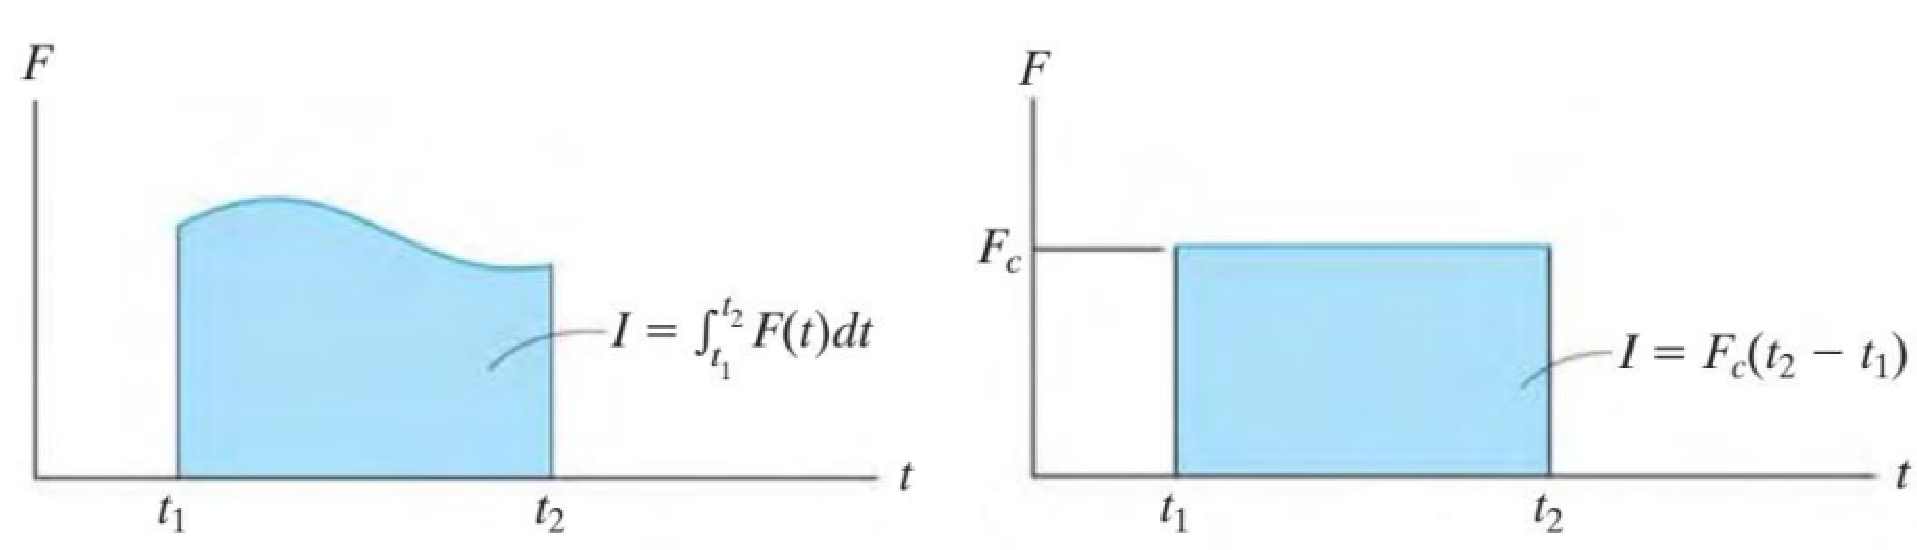
\includegraphics[width=0.5\textwidth]{db38.pdf}
  \caption{Fuerza variable (1) y fuerza constante (2)}
  \label{db38}
\end{figure}

\subsubsection{Principio de impulso y cantidad de movimiento lineales}
Para resolver
problemas la ecuación del principio se reescribe como
\begin{equation}
    mv_1 +\sum \int_{t1}^{t2}D\,dt = v_2
\end{equation}
la cual expresa que la cantidad de movimiento inicial de la partícula en el
instante $t_1$ más la suma de todos los impulsos aplicados a la partícula de $t_1$ a
$t_2$ equivale a la cantidad de movimiento final de la partícula en el instante $t_2$
Ecuaciones escalares de impulso y cantidad de
movimiento lineales

\begin{align}
    &M\left(v_x\right)_1 +\sum \int_{t1}^{t2}F_x\,dt = m\left(v_x\right)_2\\
    &M\left(v_y\right)_1 +\sum \int_{t1}^{t2}F_y\,dt = m\left(v_y\right)_2\\
    &M\left(v_z\right)_1 +\sum \int_{t1}^{t2}F_z\,dt = m\left(v_z\right)_2
\end{align}

\begin{figure}[h!]
\centering
  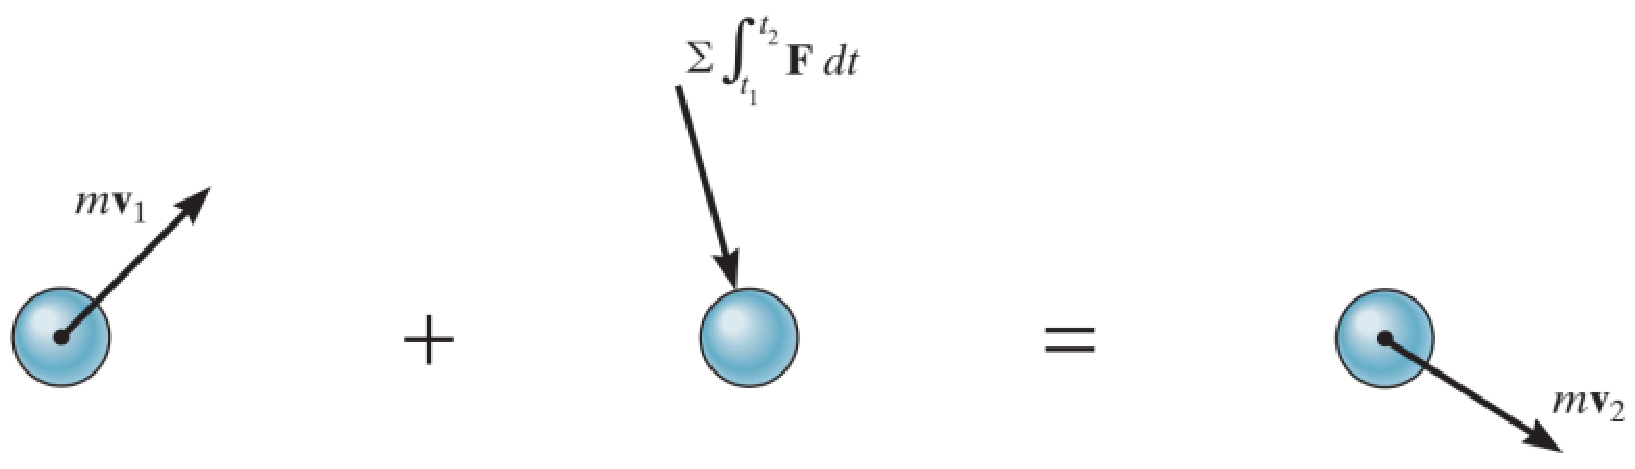
\includegraphics[width=0.5\textwidth]{db39.pdf}
  \caption{Diagrama del momentum inicial más impulso, igual a momentum final}
  \label{db39}
\end{figure}
Principio de impulso y cantidad de movimiento lineales para un sistema de
partículas. Ecuación de movimiento aplicada a todas las partículas
\begin{equation}
    \sum F_i=\sum m_i \frac{dv_i}{dt}
\end{equation}
Al multiplicar ambos lados de la ecuación por $dt$ e integrar se obtiene
\begin{equation*}
    \sum m_i(v_i)_1\, \sum \int_{t1}^{t2}F_i\,dt =\sum m_i(v_i)_2
\end{equation*}
Ubicación del centro de masa $mr_g=\sum m_ir_i$ donde $m=\sum m_i$. Derivando con respecto al tiempo
\begin{equation*}
    mv_G =\sum m_iv_i
\end{equation*}
Al sustituir se obtiene
\begin{equation*}
    m(V_g)_1 +\sum \int_{t1}^{t2}F_i\,dt = (v_G)_2
\end{equation*}
\begin{example}
    Un helicóptero de 1200 kg parte desde el reposo en el tiempo $t=0$. Las
componentes de la fuerza total (en newtons) sobre el helicóptero desde $t=0$ hasta
$t=10s$ son $\sum F_x=720t,\, \sum F_y=2160-360t$, y $\sum F_z=0$. Determine la velocidad
del helicóptero en $t= 10 s$.
\end{example}
\textit{ Sol. }

Principio del impulso y cantidad de movimiento lineales
\begin{align*}
    &mv_1 \sum \int_{t1}^{t2}F\,dt mv_2\\
    &(1200)(0) +\int_0^{10}\left(720ti +(2160 - 360t)j\right)\,dt =(1200)v_2\\
    &\left[360t^2i (2160t - 180t^2)j\right]_0^{10} =1200v_2\\ 
    &36000i 3600j = 1200v_2\\
    &v_{2} =30i +3j\frac{m}{s}
\end{align*}

\subsection{Cantidad de movimiento angular}

La cantidad de movimiento angular (momento de cantidad de movimiento) de una partícula con respecto a un punto O se define como el ``momento'' de la cantidad de movimiento lineal de la partícula con respecto a O.

\begin{definition}[Formulación escalar]
    (Cuando la partícula se mueve a lo largo de una curva situada en el plano x-y). La magnitud de $H$, es:
\begin{equation}
    (H_O)_z = (d)(mv)
\end{equation}
donde $d$ es el brazo del momento o distancia perpendicular de $O$ a la línea de acción de $mv$. Unidades para $(H_O)_z$: kg: $m^2/s$ o $slug-pie^2/s$. La dirección de $H_O$ se define por medio de la regla de la mano derecha.
\end{definition}

\begin{definition}[Formulación vectorial]
    Si la partícula se mueve a lo largo de una curva espacial, el producto vectorial puede utilizarse para determinar la cantidad de movimiento angular con respecto a O
    \begin{equation}
        H_0 = 
    \end{equation}
\end{definition}
\subsection{Cantidad de movimiento angular}

La cantidad de movimiento angular (momento de cantidad de movimiento) de una partícula con respecto a un punto $O$, $H_o$, se define como el ``momento'' de la cantidad de movimiento lineal de la partícula con respecto a $O$.

\textbf{Formulación escalar}. Si la partícula se mueve a lo largo de

una curva situada en el plano $x-y$, la magnitud de $H_0$ es:

\begin{equation}
    (H_o)_z = (d)(mv)
\end{equation}

donde $d$ es el brazo del momento o distancia perpendicular de $O$ a la línea de acción de $mv$. Unidades para $(H_o): kg m^2/s$ o $slug-pie^2/s$. La dirección de $H_o$ se define por medio de la regla de la mano derecha.
\begin{figure}[h!]
\centering
  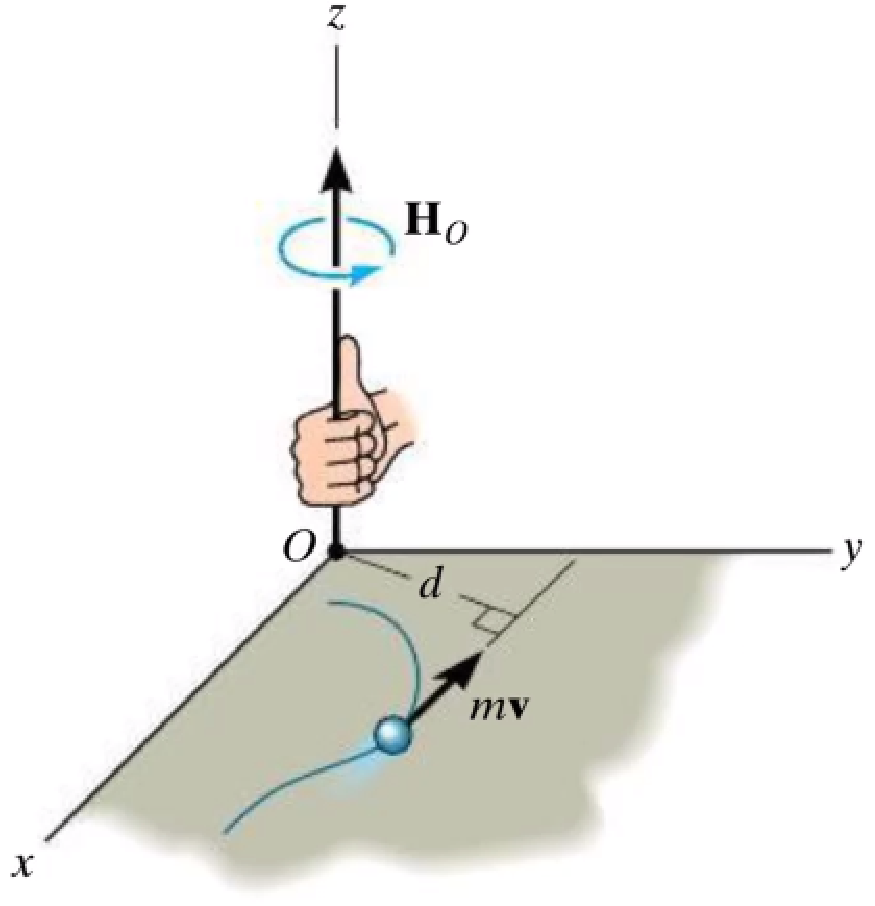
\includegraphics[width=0.5\textwidth]{db40.pdf}
  \caption{Cantidad de movimiento angular}
  \label{db40}
\end{figure}

\textbf{Formulación vectorial}. Si la partícula se mueve a lo largo de una curva espacial, la cantidad de movimiento angular con respecto a $O$, se determina con:

\begin{equation}
    H_o = r \times mv
\end{equation}

donde $r$ denota el vector de posición de $P$. $H_o$ es un vector perpendicular al plano que contiene a $r$ y $mv$.

La cantidad de movimiento angular se determina al evaluar el determinante:

\begin{equation}
    H_o = \begin{bmatrix}
        i&j&k\\
        r_x&r_y&r_z\\
        mv_x&mv_y&mv_z
    \end{bmatrix}
\end{equation}

La magnitud de $H_o$:

\begin{equation}
    H_o = mv \sin{(\phi)} 
\end{equation}

donde es el ángulo entre $r$ y $mv$. El sentido de $H_o$ puede determinarse a partir del sentido de mv aplicando la regla de la mano derecha.
\begin{figure}[h!]
\centering
  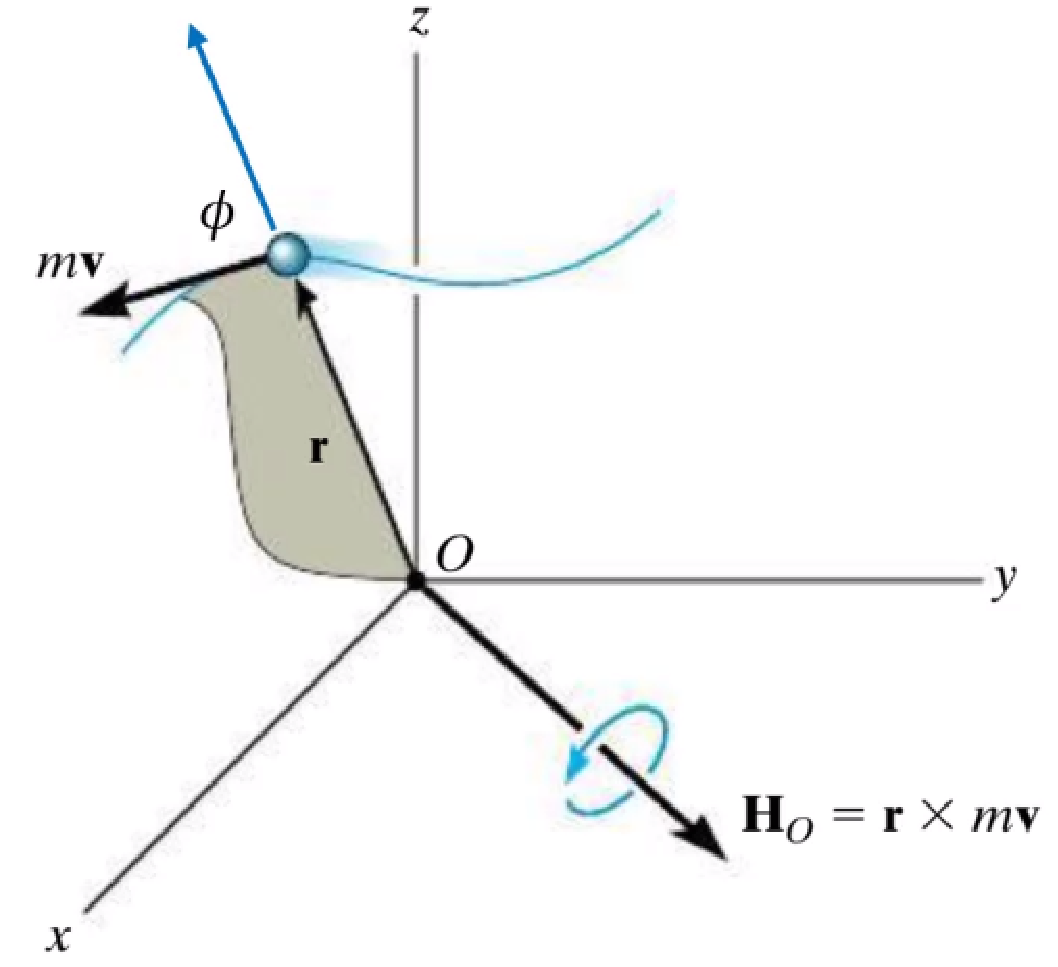
\includegraphics[width=0.5\textwidth]{db41.pdf}
  \caption{Formulación vectorial}
  \label{db41}
\end{figure}

\subsection{Relación entre el momento de una fuerza y la cantidad de movimiento angular}

Si la masa $m$ de la partícula es constante: $\sum F= m\dot{v}$. Los momentos de las fuerzas con respecto al punto O:
\begin{equation}
    \sum M_o = r \times \sum F = r \times m\dot{v}
\end{equation}
donde $r$ es el vector de posición de $P$. Derivada de $H_o$:
\begin{equation}
    H_o = \frac{d}{dt}\left(r \times mv\right) =\dot{r} \times mv + r \times m\dot{v}
\end{equation}
el primer término del lado derecho: $\dot{r}\times mv = m(\dot{r} \times  \dot{r}) = 0$, entonces, $\dot{H}_O= r\times mv$. La ecuación anterior se escribe
\begin{equation}
    \sum M_O = \dot{H}_O
\end{equation}
que establece que el momento resultante con respecto al punto O de todas las fuerzas que actúan en la partícula es igual al cambio con respecto al tiempo de la cantidad de movimiento angular con respecto al punto O.
\begin{figure}[h!]
\centering
  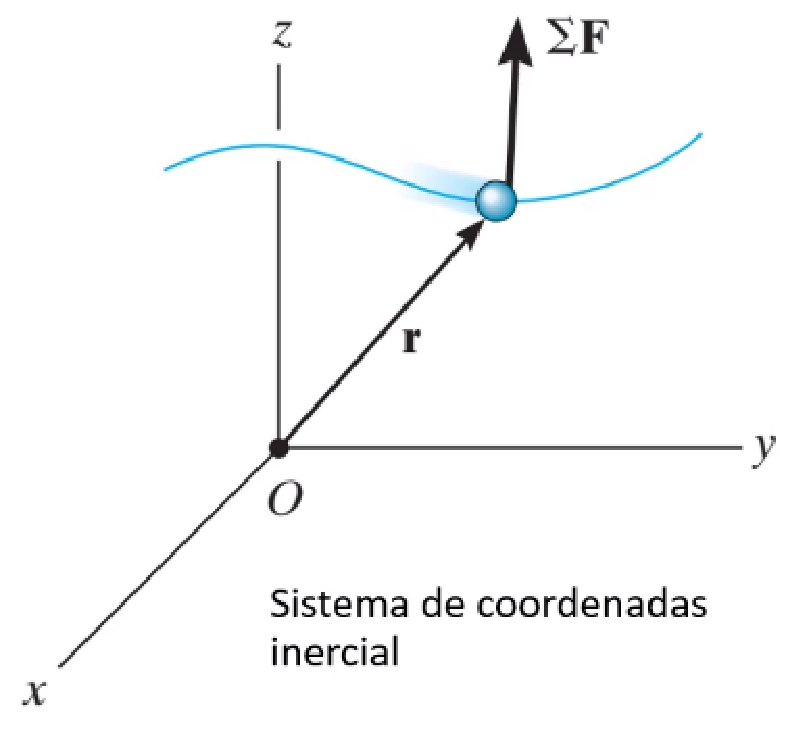
\includegraphics[width=0.5\textwidth]{db42.pdf}
  \caption{Sistema de coordenadas inercial}
  \label{db42}
\end{figure}


Sistema de partículas. Para una partícula i ésima, actúan una fuerza externa resultante F, y una fuerza interna resultante $f_1$. Los momentos de estas fuerzas con respecto al punto 0:

\begin{align*}
    &\sum M_o = \dot{H}_o\\
    &\left(r_i \times F_i\right) +\left(r_i \times f_i\right) =\left(\dot{H}_i\right)_o
\end{align*}
Sumando vectorialmente los momentos para las partículas del sistema:
\begin{equation*}
    \sum (r_i \times  F_i) + \sum (r_i \times  f_i) = \sum (\dot{H}_i)_o
\end{equation*}

El término $\sum (r_i x f_i)=0$. La ecuación anterior se escribe en forma simplificada
\begin{equation}
    \sum M_o = \dot{H}_O
\end{equation}
que establece que la suma de los momentos con respecto al punto $O$ de todas las fuerzas externas que actúan en un sistema de partículas es igual al cambio con respecto al tiempo de la cantidad de movimiento angular total del sistema con respecto al punto 0. El punto 0 puede representar cualquier punto fijo en el marco de referencia inercial.
\begin{figure}[h!]
\centering
  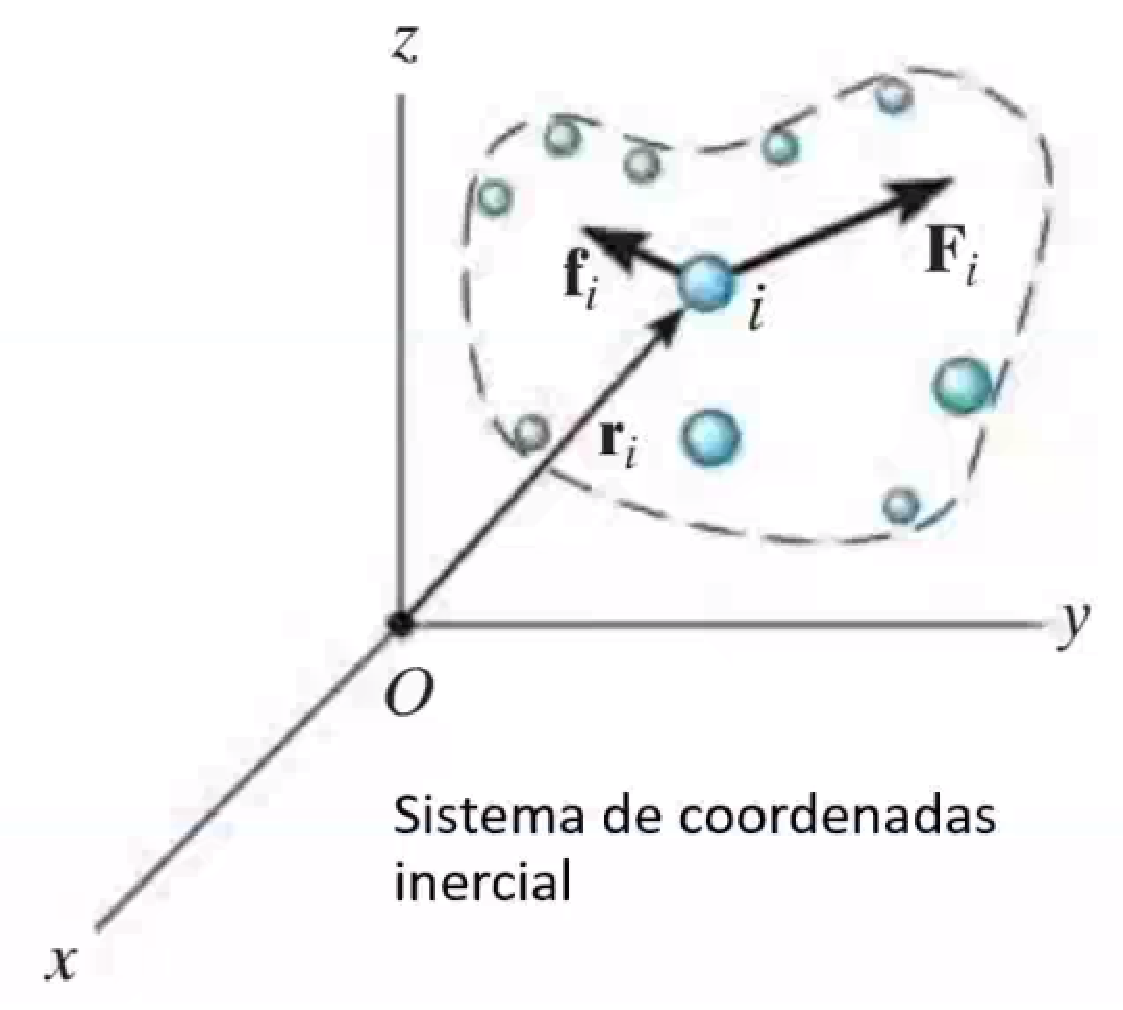
\includegraphics[width=0.5\textwidth]{db43.pdf}
  \caption{Sistema de coordenadas inercial}
  \label{db43}
\end{figure}

\subsection{Principio de impulso de impulso y cantidad de movimiento angulares}

Principio de impulso y cantidad de movimiento angulares. Si la ecuación $\sum M_o=\dot{H}_o$ se reescribe como $\sum M_o\,dt=d H_o$ y se integra, al suponer que en el instante $t=t_1$, $H_o=\left(H_o\right)_1$ y en el instante $t=t_2$, $H_o=\left(H_o\right)_2$, entonces:
\begin{equation}
    \sum \int_{t_1}^{t_2} M_o\,dt = \left(H_o\right)_2 - \left(H_o\right)_1
\end{equation}
Ecuación que se conoce como el principio de impulso y cantidad de movimiento angulares.
El principio de impulso y cantidad de movimiento angulares para un sistema de partículas:
\begin{equation}
\sum \left(H_o\right)_1 + \sum \int_{t_1}^{t_2}M_o\,dt =\sum\left(H_o\right)_2
\end{equation}